\documentclass[10pt,aspectratio=43]{beamer} 
\usepackage{hyperref}
%\usepackage{ctex} %导入中文包
\usepackage{xeCJK}
\usepackage{NJUPT}
\setCJKsansfont{SimHei} 
\setsansfont{Times New Roman}
\setmainfont{Microsoft YaHei}
\usefonttheme[onlymath]{serif}
% other packages
\usepackage{latexsym,amsmath,xcolor,multicol,booktabs,calligra}
\usepackage{graphicx,pstricks,listings,stackengine}
\usepackage[linesnumbered,vlined]{algorithm2e}
%\usepackage[linesnumbered,ruled,vlined]{algorithm2e}
\usepackage{float}
% \usepackage{emoji}


\author{雷尚远}
\title{定向覆盖模糊测试工具的设计与实现}
\subtitle{毕业设计检查}
\institute{南京邮电大学计算机学院}
\date{2023年6月}


% defs
\def\cmd#1{\texttt{\color{red}\footnotesize $\backslash$#1}}
\def\env#1{\texttt{\color{blue}\footnotesize #1}}
\definecolor{deepblue}{rgb}{0,0,0.5}
\definecolor{deepred}{rgb}{0.6,0,0}
\definecolor{deepgreen}{rgb}{0,0.5,0}
\definecolor{halfgray}{gray}{0.55}
\definecolor{red_1}{rgb}{238, 34, 12}


\lstset{
    basicstyle=\ttfamily\small,
    keywordstyle=\bfseries\color{deepblue},
    emphstyle=\ttfamily\color{deepred},    % Custom highlighting style
    stringstyle=\color{deepgreen},
    numbers=left,
    numberstyle=\small\color{halfgray},
    rulesepcolor=\color{red!20!green!20!blue!20},
    frame=shadowbox,
}


\begin{document}

\begin{frame}
    \titlepage
    \begin{figure}[htpb]
        \begin{center}
            
\includegraphics[width=0.2\linewidth]{pic/NJUPT_Logo.pdf}
        \end{center}
    \end{figure}
\end{frame}

\begin{frame}
    \tableofcontents[sectionstyle=show,subsectionstyle=show/shaded/hide,subsubsectionstyle=show/shaded/hide]
\end{frame}


\section{Background}
\subsection{Pre-Knowledge}
\begin{frame}[fragile] {What Fuzzing is?}
    \only<1>{
        \structure {Defination\cite{manes2019art}}
        \begin{itemize} 
            \item \textbf{Fuzzing} Fuzzing is the execution of the PUT using input(s) sampled from an input space (the “fuzz input space”) 
                that protrudes the expected input space of the PUT.
                \\ - PUT: Program Under Test
            \item \textbf{Fuzz testing} Fuzz testing is the use of fuzzing to test if a PUT violates a correctness policy.
            \item \textbf{Fuzzer} A fuzzer is a program that performs fuzz testing on a PUT.
            \item \textbf{Bug Oracle} A bug oracle is a program, perhaps as part of a fuzzer, that determines whether a given execution 
            of the PUT violates a specific correctness policy.
            \item \textbf{Fuzz Configuration}  A fuzz configuration of a fuzz algorithm comprises the parameter value(s) that control(s) the fuzz algorithm.
            \item \textbf{Seed} A seed is a (commonly well-structured) input to the PUT, used to generate test cases by modifying it.
        \end{itemize}
    } 
    \only<2>{
            \begin{block}{Fuzz Testing}
            \begin{algorithm}[H]
                \small
                \DontPrintSemicolon
                \SetKwSty{algokeywordsty}
                \SetFuncSty{algofuncsty}
                \SetDataSty{algodatasty}
                \SetArgSty{algoargsty}
                \SetCommentSty{algocmtsty}
                \SetKw{break}{break}
                \SetKw{not}{not}
                \SetKwFunction{preprocess}{\textsc{Preprocess}}
                \SetKwFunction{schedule}{\textsc{Schedule}}
                \SetKwFunction{inputGen}{\textsc{InputGen}}
                \SetKwFunction{inputEval}{\textsc{InputEval}}
                \SetKwFunction{confUpdate}{\textsc{ConfUpdate}}
                \SetKwFunction{continue}{\textsc{Continue}}
                \SetKwFunction{isBug}{isBug}
                \SetKwFunction{getProgram}{getProgram}
                \SetKwData{newbugs}{$\bugs^\prime$}
                \KwIn{\confs, \timeout}
                \KwOut{\bugs \tcp{a finite set of bugs}}
                $\bugs \gets \varnothing$\;
                $\confs \gets \preprocess{$\confs$}$\;
                \While {$\currtime < \timeout \land \continue{\confs}$}{
                  \conf $\gets \schedule{\confs, \currtime, \timeout}$\;
                  \testcases $\gets \inputGen{\conf}$\;
                  \tcp{\bugoracle is embedded in a fuzzer}
                  \newbugs, \execinfos $\gets$ \inputEval{\conf, \testcases, \bugoracle}\;
                  $\confs \gets \confUpdate{\confs, \conf, \execinfos}$\;
                  $\bugs \gets \bugs \cup \newbugs$\;
                }
                \Return{\bugs}\;
                %\caption[short]{fuzz testing}
            \end{algorithm} 
        \end{block}
    } 
\end{frame}

\begin{frame}{Fuzzing Algorithm}
    \only<1>{
        \begin{minipage}[t]{0.57\textwidth}
        \vspace{0pt}
        \centering
        \begin{algorithm}[H]
            \scriptsize
            \DontPrintSemicolon
            \SetKwSty{algokeywordsty}
            \SetFuncSty{algofuncsty}
            \SetDataSty{algodatasty}
            \SetArgSty{algoargsty}
            \SetCommentSty{algocmtsty}
            \SetKw{break}{break}
            \SetKw{not}{not}
            \SetKwFunction{preprocess}{\textsc{Preprocess}}
            \SetKwFunction{schedule}{\textsc{Schedule}}
            \SetKwFunction{inputGen}{\textsc{InputGen}}
            \SetKwFunction{inputEval}{\textsc{InputEval}}
            \SetKwFunction{confUpdate}{\textsc{ConfUpdate}}
            \SetKwFunction{continue}{\textsc{Continue}}
            \SetKwFunction{isBug}{isBug}
            \SetKwFunction{getProgram}{getProgram}
            \SetKwData{newbugs}{$\bugs^\prime$}
            \HiLi \KwIn{\confs, \timeout}
            \HiLi \KwOut{\bugs \tcp{a finite set of bugs}}
            $\bugs \gets \varnothing$\;
            $\confs \gets \preprocess{$\confs$}$\;
            \While {$\currtime < \timeout \land \continue{\confs}$}{
              \conf $\gets \schedule{\confs, \currtime, \timeout}$\;
              \testcases $\gets \inputGen{\conf}$\;
              \tcp{\bugoracle is embedded in a fuzzer}
              \newbugs, \execinfos $\gets$ \inputEval{\conf, \testcases, \bugoracle}\;
              $\confs \gets \confUpdate{\confs, \conf, \execinfos}$\;
              $\bugs \gets \bugs \cup \newbugs$\;
            }
            \Return{\bugs}\;
        \end{algorithm} 
        \end{minipage} 
        \begin{minipage}[t]{0.4\textwidth}
            {
                \vspace{25pt}
                \centering
                \footnotesize{
                    \begin{itemize}  
                        \item  \confs :a set of fuzz configurations
                        \item  \timeout: timeout
                        \item  \bugs: a set of discovered bugs
                    \end{itemize} 
                }
            }
        \end{minipage}
    }  

    \only<2>{
        \begin{minipage}[t]{0.57\linewidth}
        \vspace{0pt}
        \centering
        \begin{algorithm}[H]
            \scriptsize
            \DontPrintSemicolon
            \SetKwSty{algokeywordsty}
            \SetFuncSty{algofuncsty}
            \SetDataSty{algodatasty}
            \SetArgSty{algoargsty}
            \SetCommentSty{algocmtsty}
            \SetKw{break}{break}
            \SetKw{not}{not}
            \SetKwFunction{preprocess}{\textsc{Preprocess}}
            \SetKwFunction{schedule}{\textsc{Schedule}}
            \SetKwFunction{inputGen}{\textsc{InputGen}}
            \SetKwFunction{inputEval}{\textsc{InputEval}}
            \SetKwFunction{confUpdate}{\textsc{ConfUpdate}}
            \SetKwFunction{continue}{\textsc{Continue}}
            \SetKwFunction{isBug}{isBug}
            \SetKwFunction{getProgram}{getProgram}
            \SetKwData{newbugs}{$\bugs^\prime$}
            \KwIn{\confs, \timeout}
            \KwOut{\bugs \tcp{a finite set of bugs}}
            \HiLi$\bugs \gets \varnothing$\;
            \HiLi$\confs \gets \preprocess{$\confs$}$\;
            \While {$\currtime < \timeout \land \continue{\confs}$}{
              \conf $\gets \schedule{\confs, \currtime, \timeout}$\;
              \testcases $\gets \inputGen{\conf}$\;
              \tcp{\bugoracle is embedded in a fuzzer}
              \newbugs, \execinfos $\gets$ \inputEval{\conf, \testcases, \bugoracle}\;
              $\confs \gets \confUpdate{\confs, \conf, \execinfos}$\;
              $\bugs \gets \bugs \cup \newbugs$\;
            }
            \Return{\bugs}\;
        \end{algorithm} 
        \end{minipage} 
        \begin{minipage}[t]{0.4\linewidth}
            \vspace{0pt}
            \centering
            \preprocess\normalfont(\confs) $\rightarrow \confs$ 
            \scriptsize{
            \begin{itemize}
                \item  \textbf{Instrumentation}
                    \\- grey-box and white-box fuzzers
                    \\- \alert{static}/dynamic(\inputEval)
                \item \textbf{Seed Selection}
                    \\- weed out potentially redundant configurations
                \item  \textbf{Seed Trimming}
                    \\- reduce the size of seeds
                \item  \textbf{Preparing a Driver Application}
                     \\- library Fuzzing, kernal Fuzzing
            \end{itemize}
            } 
        \end{minipage}
    }
   
    \only<3>{
        \begin{minipage}[t]{0.57\linewidth}
        \vspace{0pt}
        \centering
        \begin{algorithm}[H]
            \scriptsize
            \DontPrintSemicolon
            \SetKwSty{algokeywordsty}
            \SetFuncSty{algofuncsty}
            \SetDataSty{algodatasty}
            \SetArgSty{algoargsty}
            \SetCommentSty{algocmtsty}
            \SetKw{break}{break}
            \SetKw{not}{not}
            \SetKwFunction{preprocess}{\textsc{Preprocess}}
            \SetKwFunction{schedule}{\textsc{Schedule}}
            \SetKwFunction{inputGen}{\textsc{InputGen}}
            \SetKwFunction{inputEval}{\textsc{InputEval}}
            \SetKwFunction{confUpdate}{\textsc{ConfUpdate}}
            \SetKwFunction{continue}{\textsc{Continue}}
            \SetKwFunction{isBug}{isBug}
            \SetKwFunction{getProgram}{getProgram}
            \SetKwData{newbugs}{$\bugs^\prime$}
            \KwIn{\confs, \timeout}
            \KwOut{\bugs \tcp{a finite set of bugs}}
            $\bugs \gets \varnothing$\;
            $\confs \gets \preprocess{$\confs$}$\;
            \HiLi\While {$\currtime < \timeout \land \continue{\confs}$}{
              \conf $\gets \schedule{\confs, \currtime, \timeout}$\;
              \testcases $\gets \inputGen{\conf}$\;
              \tcp{\bugoracle is embedded in a fuzzer}
              \newbugs, \execinfos $\gets$ \inputEval{\conf, \testcases, \bugoracle}\;
              $\confs \gets \confUpdate{\confs, \conf, \execinfos}$\;
              $\bugs \gets \bugs \cup \newbugs$\;
            }
            \Return{\bugs}\;
        \end{algorithm} 
        \end{minipage}
        \begin{minipage}[t]{0.4\linewidth}
            {
                \vspace{25pt}
                \centering
                    Stop Condition
                    \scriptsize{
                        \begin{itemize}  
                            \item  $\currtime < \timeout$
                            \item  \continue\normalfont(\confs)$\rightarrow \{\texttt{True}, \texttt{False}\}$
                            \\- Determine whether a new fuzz iteration should occur
                        \end{itemize} 
                    }
            }
        \end{minipage}
    }

    \only<4>{
        \begin{minipage}[t]{0.57\linewidth}
        \vspace{0pt}
        \centering
        \begin{algorithm}[H]
            \scriptsize
            \DontPrintSemicolon
            \SetKwSty{algokeywordsty}
            \SetFuncSty{algofuncsty}
            \SetDataSty{algodatasty}
            \SetArgSty{algoargsty}
            \SetCommentSty{algocmtsty}
            \SetKw{break}{break}
            \SetKw{not}{not}
            \SetKwFunction{preprocess}{\textsc{Preprocess}}
            \SetKwFunction{schedule}{\textsc{Schedule}}
            \SetKwFunction{inputGen}{\textsc{InputGen}}
            \SetKwFunction{inputEval}{\textsc{InputEval}}
            \SetKwFunction{confUpdate}{\textsc{ConfUpdate}}
            \SetKwFunction{continue}{\textsc{Continue}}
            \SetKwFunction{isBug}{isBug}
            \SetKwFunction{getProgram}{getProgram}
            \SetKwData{newbugs}{$\bugs^\prime$}
            \KwIn{\confs, \timeout}
            \KwOut{\bugs \tcp{a finite set of bugs}}
            $\bugs \gets \varnothing$\;
            $\confs \gets \preprocess{$\confs$}$\;
            \While {$\currtime < \timeout \land \continue{\confs}$}{
             \HiLi  \conf $\gets \schedule{\confs, \currtime, \timeout}$\;
              \testcases $\gets \inputGen{\conf}$\;
              \tcp{\bugoracle is embedded in a fuzzer}
              \newbugs, \execinfos $\gets$ \inputEval{\conf, \testcases, \bugoracle}\;
              $\confs \gets \confUpdate{\confs, \conf, \execinfos}$\;
              $\bugs \gets \bugs \cup \newbugs$\;
            }
            \Return{\bugs}\;
        \end{algorithm} 
        \end{minipage} 
        \begin{minipage}[t]{0.4\linewidth}
            {
                \vspace{0pt}
                \centering
                \scriptsize{
                \schedule\normalfont(\confs, \currtime, \timeout) $\rightarrow \conf$
                    \begin{itemize} 
                        \item \textbf{Function}
                            \\- Pick important information(\conf )
                        \item \textbf{FCS Problem} 
                            \\- \textit{exploration}:Spent time on gathering more accurate information on each configuration to inform future decisions
                            \\- \textit{exploitation}:Spent time on fuzzing the configurations that are currently believed to lead to more favorable outcomes
                    \end{itemize} 
                }
            }
        \end{minipage}
    }


    \only<5>{
        \begin{minipage}[t]{0.57\linewidth}
        \vspace{0pt}
        \centering
        \begin{algorithm}[H]
            \scriptsize
            \DontPrintSemicolon
            \SetKwSty{algokeywordsty}
            \SetFuncSty{algofuncsty}
            \SetDataSty{algodatasty}
            \SetArgSty{algoargsty}
            \SetCommentSty{algocmtsty}
            \SetKw{break}{break}
            \SetKw{not}{not}
            \SetKwFunction{preprocess}{\textsc{Preprocess}}
            \SetKwFunction{schedule}{\textsc{Schedule}}
            \SetKwFunction{inputGen}{\textsc{InputGen}}
            \SetKwFunction{inputEval}{\textsc{InputEval}}
            \SetKwFunction{confUpdate}{\textsc{ConfUpdate}}
            \SetKwFunction{continue}{\textsc{Continue}}
            \SetKwFunction{isBug}{isBug}
            \SetKwFunction{getProgram}{getProgram}
            \SetKwData{newbugs}{$\bugs^\prime$}
            \KwIn{\confs, \timeout}
            \KwOut{\bugs \tcp{a finite set of bugs}}
            $\bugs \gets \varnothing$\;
            $\confs \gets \preprocess{$\confs$}$\;
            \While {$\currtime < \timeout \land \continue{\confs}$}{
            \conf $\gets \schedule{\confs, \currtime, \timeout}$\;
            \HiLi\testcases $\gets \inputGen{\conf}$\;
              \tcp{\bugoracle is embedded in a fuzzer}
              \newbugs, \execinfos $\gets$ \inputEval{\conf, \testcases, \bugoracle}\;
              $\confs \gets \confUpdate{\confs, \conf, \execinfos}$\;
              $\bugs \gets \bugs \cup \newbugs$\;
            }
            \Return{\bugs}\;
        \end{algorithm} 
        \end{minipage} 
        \begin{minipage}[t]{0.4\linewidth}
            {
                \vspace{25pt}
                \centering
                \scriptsize{
                    \inputGen\normalfont(\conf)$\rightarrow \testcases$ 
                    \begin{itemize}  
                        \item \textbf{function}
                            \\- Generate testcases
                        \item  \textbf{classification}
                            \\- Generation-based(\textit{Model-based})
                            \\- Mutation-based(\textit{Model-less})
                            \\- White-box Fuzzers: symbolic execution
                    \end{itemize} 
                }
            }
        \end{minipage}
    }

    \only<6>{
        \begin{minipage}[t]{0.57\linewidth}
        \vspace{0pt}
        \centering
        \begin{algorithm}[H]
            \scriptsize
            \DontPrintSemicolon
            \SetKwSty{algokeywordsty}
            \SetFuncSty{algofuncsty}
            \SetDataSty{algodatasty}
            \SetArgSty{algoargsty}
            \SetCommentSty{algocmtsty}
            \SetKw{break}{break}
            \SetKw{not}{not}
            \SetKwFunction{preprocess}{\textsc{Preprocess}}
            \SetKwFunction{schedule}{\textsc{Schedule}}
            \SetKwFunction{inputGen}{\textsc{InputGen}}
            \SetKwFunction{inputEval}{\textsc{InputEval}}
            \SetKwFunction{confUpdate}{\textsc{ConfUpdate}}
            \SetKwFunction{continue}{\textsc{Continue}}
            \SetKwFunction{isBug}{isBug}
            \SetKwFunction{getProgram}{getProgram}
            \SetKwData{newbugs}{$\bugs^\prime$}
            \KwIn{\confs, \timeout}
            \KwOut{\bugs \tcp{a finite set of bugs}}
            $\bugs \gets \varnothing$\;
            $\confs \gets \preprocess{$\confs$}$\;
            \While {$\currtime < \timeout \land \continue{\confs}$}{
            \conf $\gets \schedule{\confs, \currtime, \timeout}$\;
              \testcases $\gets \inputGen{\conf}$\;
              \tcp{\bugoracle is embedded in a fuzzer}
              \HiLi  \newbugs, \execinfos $\gets$ \inputEval{\conf, \testcases, \bugoracle}\;
              $\confs \gets \confUpdate{\confs, \conf, \execinfos}$\;
              $\bugs \gets \bugs \cup \newbugs$\;
            }
            \Return{\bugs}\;
        \end{algorithm} 
        \end{minipage} 
        \begin{minipage}[t]{0.4\linewidth}
            {
                \vspace{0pt}
                \centering
                \scriptsize{
                    \inputEval\normalfont(\conf, \testcases, \bugoracle) $\rightarrow \bugs^\prime, \execinfos$  
                    \begin{itemize}  
                        \item \textbf{Fuzzing PUT}
                            \\- \testcases
                            \\- $\bugs^\prime$
                        \item \textbf{Feedback Information} 
                            \\- \conf, \testcases
                            \\- \execinfos (\testcases,crashes,stack backtrace hash,edge coverage,etc.)
                    \end{itemize} 
                }
            }
        \end{minipage}
    }

    \only<7>{
        \begin{minipage}[t]{0.57\linewidth}
        \vspace{0pt}
        \centering
        \begin{algorithm}[H]
            \scriptsize
            \DontPrintSemicolon
            \SetKwSty{algokeywordsty}
            \SetFuncSty{algofuncsty}
            \SetDataSty{algodatasty}
            \SetArgSty{algoargsty}
            \SetCommentSty{algocmtsty}
            \SetKw{break}{break}
            \SetKw{not}{not}
            \SetKwFunction{preprocess}{\textsc{Preprocess}}
            \SetKwFunction{schedule}{\textsc{Schedule}}
            \SetKwFunction{inputGen}{\textsc{InputGen}}
            \SetKwFunction{inputEval}{\textsc{InputEval}}
            \SetKwFunction{confUpdate}{\textsc{ConfUpdate}}
            \SetKwFunction{continue}{\textsc{Continue}}
            \SetKwFunction{isBug}{isBug}
            \SetKwFunction{getProgram}{getProgram}
            \SetKwData{newbugs}{$\bugs^\prime$}
            \KwIn{\confs, \timeout}
            \KwOut{\bugs \tcp{a finite set of bugs}}
            $\bugs \gets \varnothing$\;
            $\confs \gets \preprocess{$\confs$}$\;
            \While {$\currtime < \timeout \land \continue{\confs}$}{
            \conf $\gets \schedule{\confs, \currtime, \timeout}$\;
              \testcases $\gets \inputGen{\conf}$\;
              \tcp{\bugoracle is embedded in a fuzzer}
              \newbugs, \execinfos $\gets$ \inputEval{\conf, \testcases, \bugoracle}\;
              \HiLi  $\confs \gets \confUpdate{\confs, \conf, \execinfos}$\;
              \HiLi $\bugs \gets \bugs \cup \newbugs$\;
            }
            \Return{\bugs}\;
        \end{algorithm} 
        \end{minipage} 
        \begin{minipage}[t]{0.4\linewidth}
            {
                \vspace{25pt}
                \centering
                \scriptsize{
                    \begin{itemize}  
                        \item  \confUpdate\normalfont(\confs, \conf, \execinfos) $\rightarrow \confs$
                            \\- Update Fuzz Configuration(distinguishablity)
                            \\- Seed Pool Update
                        \item   $\bugs \cup \bugs^\prime \rightarrow \bugs$
                            \\- Update Bugs Set
                    \end{itemize} 
                }
            }
        \end{minipage}
    }

    \only<8>{
        \begin{minipage}[t]{0.57\linewidth}
        \vspace{0pt}
        \centering
        \begin{algorithm}[H]
            \scriptsize
            \DontPrintSemicolon
            \SetKwSty{algokeywordsty}
            \SetFuncSty{algofuncsty}
            \SetDataSty{algodatasty}
            \SetArgSty{algoargsty}
            \SetCommentSty{algocmtsty}
            \SetKw{break}{break}
            \SetKw{not}{not}
            \SetKwFunction{preprocess}{\textsc{Preprocess}}
            \SetKwFunction{schedule}{\textsc{Schedule}}
            \SetKwFunction{inputGen}{\textsc{InputGen}}
            \SetKwFunction{inputEval}{\textsc{InputEval}}
            \SetKwFunction{confUpdate}{\textsc{ConfUpdate}}
            \SetKwFunction{continue}{\textsc{Continue}}
            \SetKwFunction{isBug}{isBug}
            \SetKwFunction{getProgram}{getProgram}
            \SetKwData{newbugs}{$\bugs^\prime$}
            \KwIn{\confs, \timeout}
            \KwOut{\bugs \tcp{a finite set of bugs}}
            $\bugs \gets \varnothing$\;
            $\confs \gets \preprocess{$\confs$}$\;
            \HiLi\While {$\currtime < \timeout \land \continue{\confs}$}{
              \conf $\gets \schedule{\confs, \currtime, \timeout}$\;
              \testcases $\gets \inputGen{\conf}$\;
              \tcp{\bugoracle is embedded in a fuzzer}
              \newbugs, \execinfos $\gets$ \inputEval{\conf, \testcases, \bugoracle}\;
              $\confs \gets \confUpdate{\confs, \conf, \execinfos}$\;
              $\bugs \gets \bugs \cup \newbugs$\;
            }
            \HiLi\Return{\bugs}\;
        \end{algorithm} 
        \end{minipage} 
        \begin{minipage}[t]{0.4\linewidth}
            {
                \vspace{25pt}
                \centering
                stop condition
                \scriptsize{
                    \begin{itemize}  
                        \item  $\currtime < \timeout$
                        \item  \continue\normalfont(\confs)$\rightarrow \{\texttt{True}, \texttt{False}\}$
                        \\- Determine whether a new fuzz iteration should occur
                    \end{itemize} 
                }
            }
        \end{minipage}
    }
\end{frame}

\subsection{Motivation}
\begin{frame}{Classification}
    \only<1>{
        \begin{quote}
           The amount of collected information defines the color of a fuzzer\cite{manes2019art}.
        \end{quote}
        \begin{minipage}[t]{0.57\linewidth}
        \vspace{0pt}
        \centering
        \begin{algorithm}[H]
            \scriptsize
            \DontPrintSemicolon
            \SetKwSty{algokeywordsty}
            \SetFuncSty{algofuncsty}
            \SetDataSty{algodatasty}
            \SetArgSty{algoargsty}
            \SetCommentSty{algocmtsty}
            \SetKw{break}{break}
            \SetKw{not}{not}
            \SetKwFunction{preprocess}{\textsc{Preprocess}}
            \SetKwFunction{schedule}{\textsc{Schedule}}
            \SetKwFunction{inputGen}{\textsc{InputGen}}
            \SetKwFunction{inputEval}{\textsc{InputEval}}
            \SetKwFunction{confUpdate}{\textsc{ConfUpdate}}
            \SetKwFunction{continue}{\textsc{Continue}}
            \SetKwFunction{isBug}{isBug}
            \SetKwFunction{getProgram}{getProgram}
            \SetKwData{newbugs}{$\bugs^\prime$}
            \KwIn{\confs, \timeout}
            \KwOut{\bugs \tcp{a finite set of bugs}}
            $\bugs \gets \varnothing$\;
            \HiLi$\confs \gets \preprocess{$\confs$}$\;
            \While {$\currtime < \timeout \land \continue{\confs}$}{
              \conf $\gets \schedule{\confs, \currtime, \timeout}$\;
              \testcases $\gets \inputGen{\conf}$\;
              \tcp{\bugoracle is embedded in a fuzzer}
              \newbugs, \execinfos $\gets$ \inputEval{\conf, \testcases, \bugoracle}\;
            \HiLi $\confs \gets \confUpdate{\confs, \conf, \execinfos}$\;
              $\bugs \gets \bugs \cup \newbugs$\;
            }
            \Return{\bugs}\;
        \end{algorithm} 
        \end{minipage} 
        \begin{minipage}[t]{0.4\linewidth}
            \vspace{0pt}
            \centering 
            \scriptsize{
            \begin{itemize}
                \item  \textbf{program instrumentation}
                \scriptsize{
                    \begin{itemize}
                         \item static
                         \item dynamic 
                    \end{itemize}
                }
                \item processor traces
                \item system call usage
                \item etc.
            \end{itemize}
            } 
        \end{minipage}
    }
    \only<2>{
        \begin{minipage}[t]{0.57\linewidth}
        \vspace{0pt}
        \centering
        \begin{algorithm}[H]
            \scriptsize
            \DontPrintSemicolon
            \SetKwSty{algokeywordsty}
            \SetFuncSty{algofuncsty}
            \SetDataSty{algodatasty}
            \SetArgSty{algoargsty}
            \SetCommentSty{algocmtsty}
            \SetKw{break}{break}
            \SetKw{not}{not}
            \SetKwFunction{preprocess}{\textsc{Preprocess}}
            \SetKwFunction{schedule}{\textsc{Schedule}}
            \SetKwFunction{inputGen}{\textsc{InputGen}}
            \SetKwFunction{inputEval}{\textsc{InputEval}}
            \SetKwFunction{confUpdate}{\textsc{ConfUpdate}}
            \SetKwFunction{continue}{\textsc{Continue}}
            \SetKwFunction{isBug}{isBug}
            \SetKwFunction{getProgram}{getProgram}
            \SetKwData{newbugs}{$\bugs^\prime$}
            \KwIn{\confs, \timeout}
            \KwOut{\bugs \tcp{a finite set of bugs}}
            $\bugs \gets \varnothing$\;
            \alert{$\confs \gets \preprocess{$\confs$}$\;}
            \While {$\currtime < \timeout \land \continue{\confs}$}{
              \conf $\gets \schedule{\confs, \currtime, \timeout}$\;
              \testcases $\gets \inputGen{\conf}$\;
              \tcp{\bugoracle is embedded in a fuzzer}
              \newbugs, \execinfos $\gets$ \inputEval{\conf, \testcases, \bugoracle}\;
              $\confs \gets \confUpdate{\confs, \conf, \execinfos}$\;
              $\bugs \gets \bugs \cup \newbugs$\;
            }
            \Return{\bugs}\;
        \end{algorithm} 
        \end{minipage} 
        \begin{minipage}[t]{0.4\linewidth}
            \vspace{0pt}
            \centering 
            \textbf{Program Instrumentation}
            \scriptsize{
                \begin{itemize}
                    \item \alert{Static}
                        \\- source code
                        \\- intermediate code
                        \\- binary-level 
                    \item Dynamic 
                \end{itemize}
                }
        \end{minipage}
    }
    \only<3>{
        \begin{minipage}[t]{0.57\linewidth}
        \vspace{0pt}
        \centering
        \begin{algorithm}[H]
            \scriptsize
            \DontPrintSemicolon
            \SetKwSty{algokeywordsty}
            \SetFuncSty{algofuncsty}
            \SetDataSty{algodatasty}
            \SetArgSty{algoargsty}
            \SetCommentSty{algocmtsty}
            \SetKw{break}{break}
            \SetKw{not}{not}
            \SetKwFunction{preprocess}{\textsc{Preprocess}}
            \SetKwFunction{schedule}{\textsc{Schedule}}
            \SetKwFunction{inputGen}{\textsc{InputGen}}
            \SetKwFunction{inputEval}{\textsc{InputEval}}
            \SetKwFunction{confUpdate}{\textsc{ConfUpdate}}
            \SetKwFunction{continue}{\textsc{Continue}}
            \SetKwFunction{isBug}{isBug}
            \SetKwFunction{getProgram}{getProgram}
            \SetKwData{newbugs}{$\bugs^\prime$}
            \KwIn{\confs, \timeout}
            \KwOut{\bugs \tcp{a finite set of bugs}}
            $\bugs \gets \varnothing$\;
            $\confs \gets \preprocess{$\confs$}$\;
            \While {$\currtime < \timeout \land \continue{\confs}$}{
              \conf $\gets \schedule{\confs, \currtime, \timeout}$\;
              \testcases $\gets \inputGen{\conf}$\;
              \tcp{\bugoracle is embedded in a fuzzer}
            \alert{\newbugs, \execinfos $\gets$ \inputEval{\conf, \testcases, \bugoracle}\;}
              $\confs \gets \confUpdate{\confs, \conf, \execinfos}$\;
              $\bugs \gets \bugs \cup \newbugs$\;
            }
            \Return{\bugs}\;
        \end{algorithm} 
        \end{minipage} 
        \begin{minipage}[t]{0.4\linewidth}
            \vspace{0pt}
            \centering 
            \textbf{Program Instrumentation}
            \scriptsize{
                \begin{itemize}
                    \item Static
                    \item \alert{Dynamic} 
                        \\- dynamically-linked libraries
                        \\- execution feedback: branch coverage, new path, etc.
                        \\- race condition bugs: thread scheduling
                \end{itemize}
                }
        \end{minipage}
    }
    \only<4>{
        \structure {Classification of Fuzzing}
        \begin{itemize} 
            \item  \textbf{Black-box Fuzzing}
                \\ - no program analysis, no feedback
            \item  \textbf{White-box Fuzzing} 
                \\ - mostly program analysis
            \item  \textbf{Grey-box  Fuzzing} 
                \\ - no program analysis, but feedback
        \end{itemize} 
    }
\end{frame}
\begin{frame}{Why Grey-box Fuzzing ?}
    \only<1>{
        \begin{itemize}  
        \item \structure {Black-box Fuzzing}
        \\ \textbf{Defination:} techniques that do not see the internals of the PUT,and can observe only the input/output behavior of the PUT,
           treating it as a black-box\cite{manes2019art}.
        \\ -No \alert{program analysis}, no \alert{feedback}
        \end{itemize} 
        \begin{picture}(320,250)
            \put(-15,110){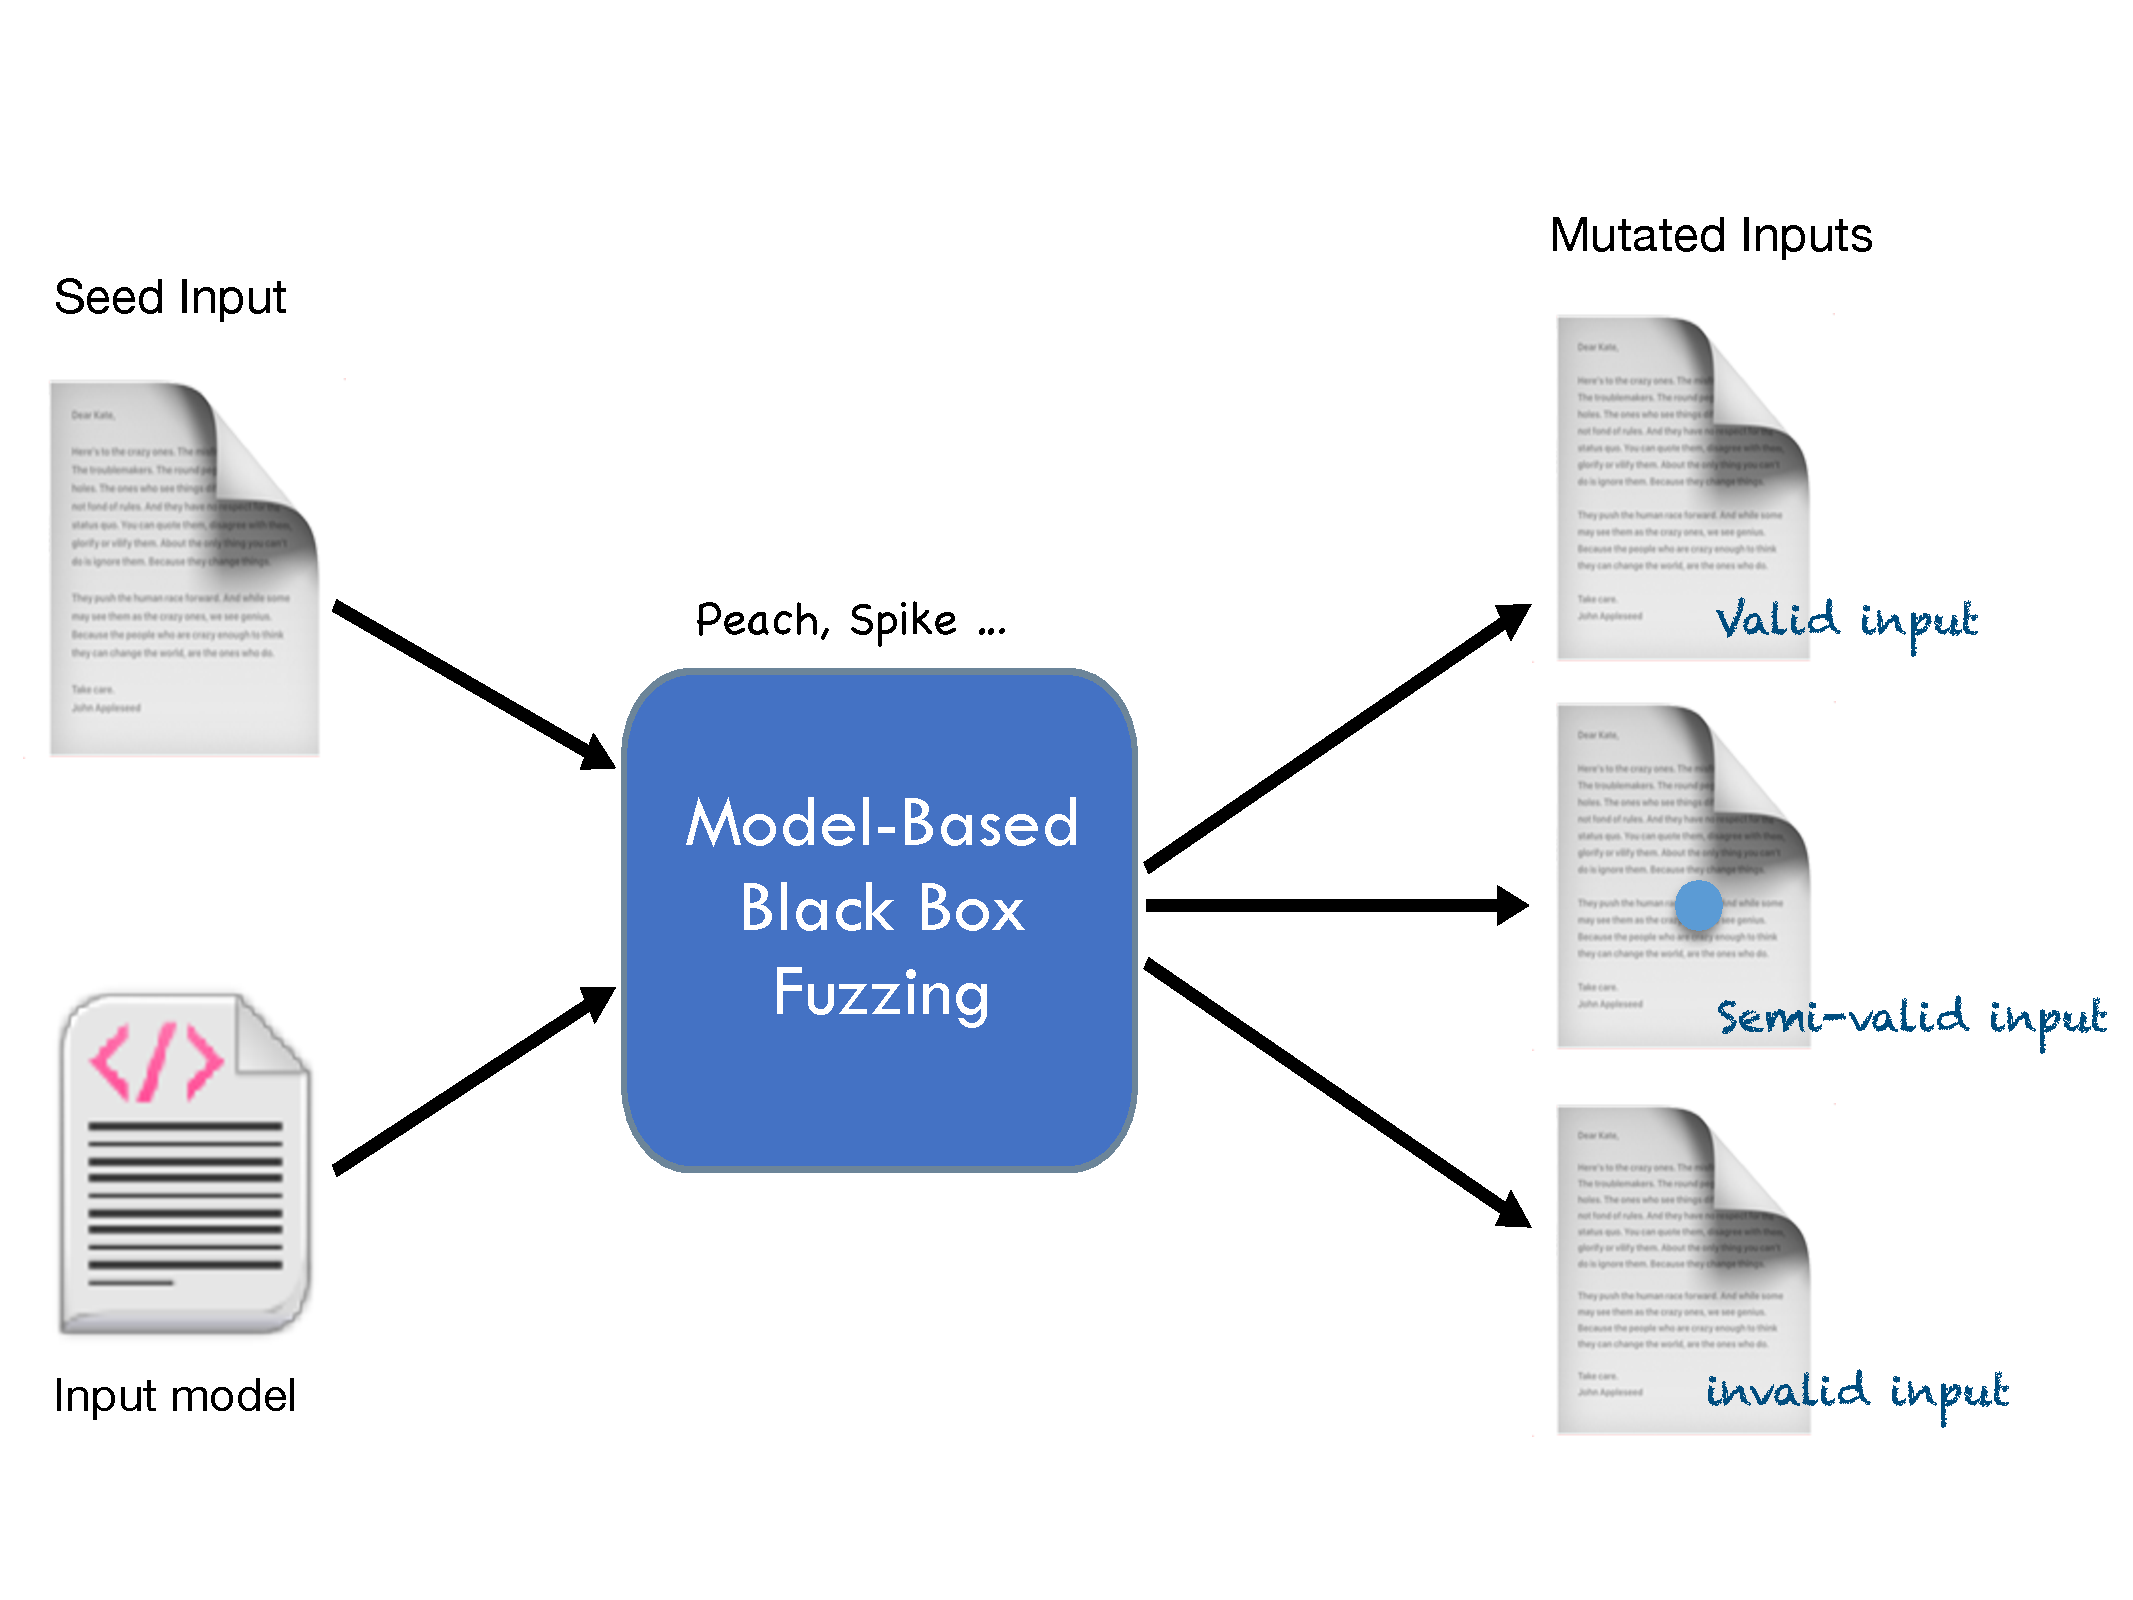
\includegraphics[width=8.0cm]{pic/blackbox.pdf}}
        \end{picture} 
    }

    \only<2>{
        \begin{itemize}  
        \item \structure {Black-box Fuzzing}
        \\ \textbf{Defination:} techniques that do not see the internals of the PUT,and can observe only the input/output behavior of the PUT,
           treating it as a black-box\cite{manes2019art}.
        \\ - No \alert{program analysis}, no \alert{feedback}
        \end{itemize} 
        \begin{picture}(320,250)
            \put(-25,110){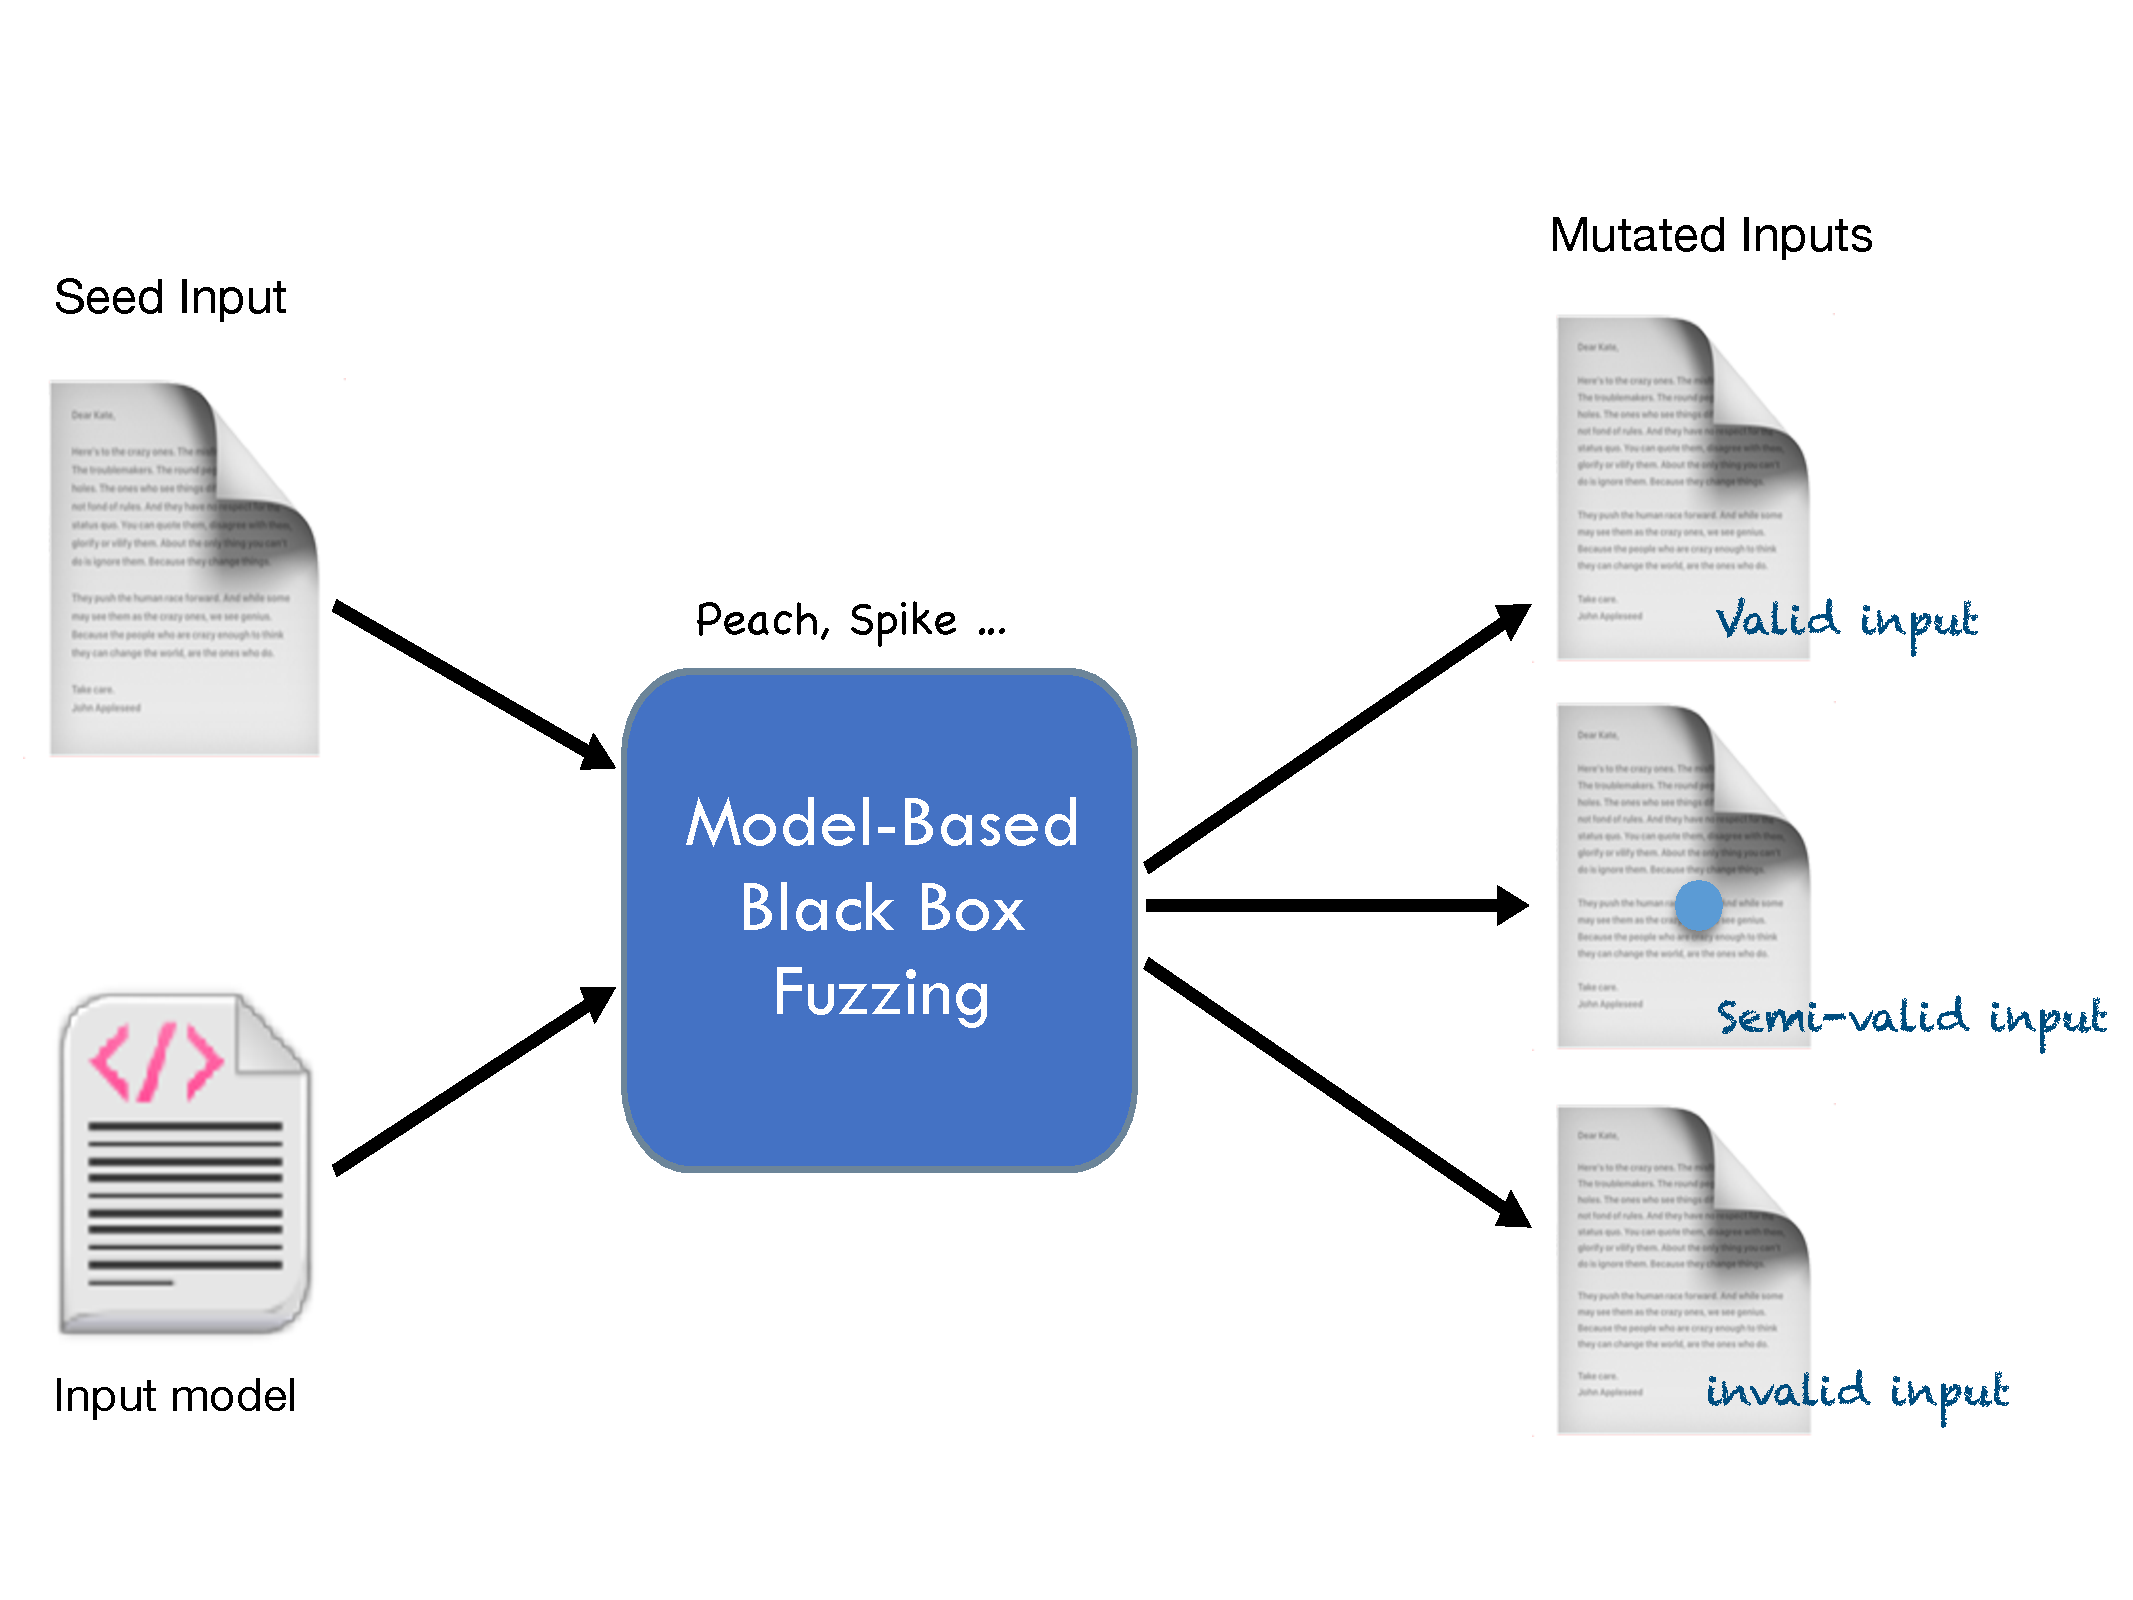
\includegraphics[width=8.0cm]{pic/blackbox.pdf}}
            \put(190,220){
                \begin{minipage}[t]{0.45\linewidth}
                {
                    \footnotesize{
                        \begin{itemize}  
                            \item  You have no view of the PUT,but have some view of the input/output domain
                            \item  Fuzzing congfigurations are not changed according to some feedback 
                                \\- some fuzzer may add the testcases to seed pool 
                            \item \alert {Not effective}
                        \end{itemize} 
                    }
                }
                \end{minipage}
                }
        \end{picture} 
    }
    \only<3>{
        \begin{itemize}  
        \item \structure {White-box Fuzzing}
          \\ \textbf{Defination:} techniques that generates test cases by analyzing the internals of the PUT and the information gathered 
          when executing the PUT\cite{manes2019art}.
          \\ - Requires heavy-weight \alert {program analysis} and constraint solving. 
        \end{itemize} 
        \begin{picture}(320,250)
            \put(-20,120){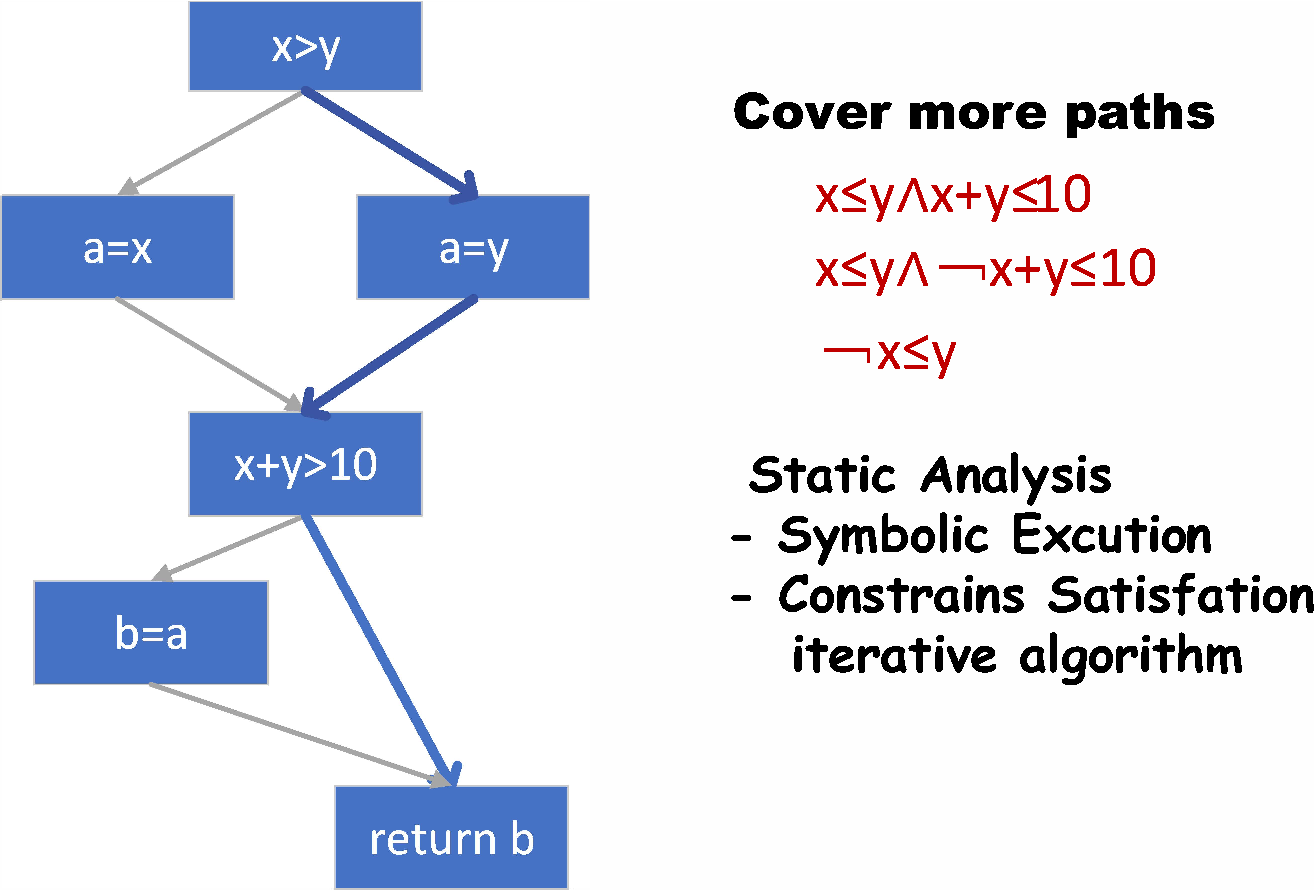
\includegraphics[width=6.0cm]{pic/cfg.pdf}}
            \put(160,120){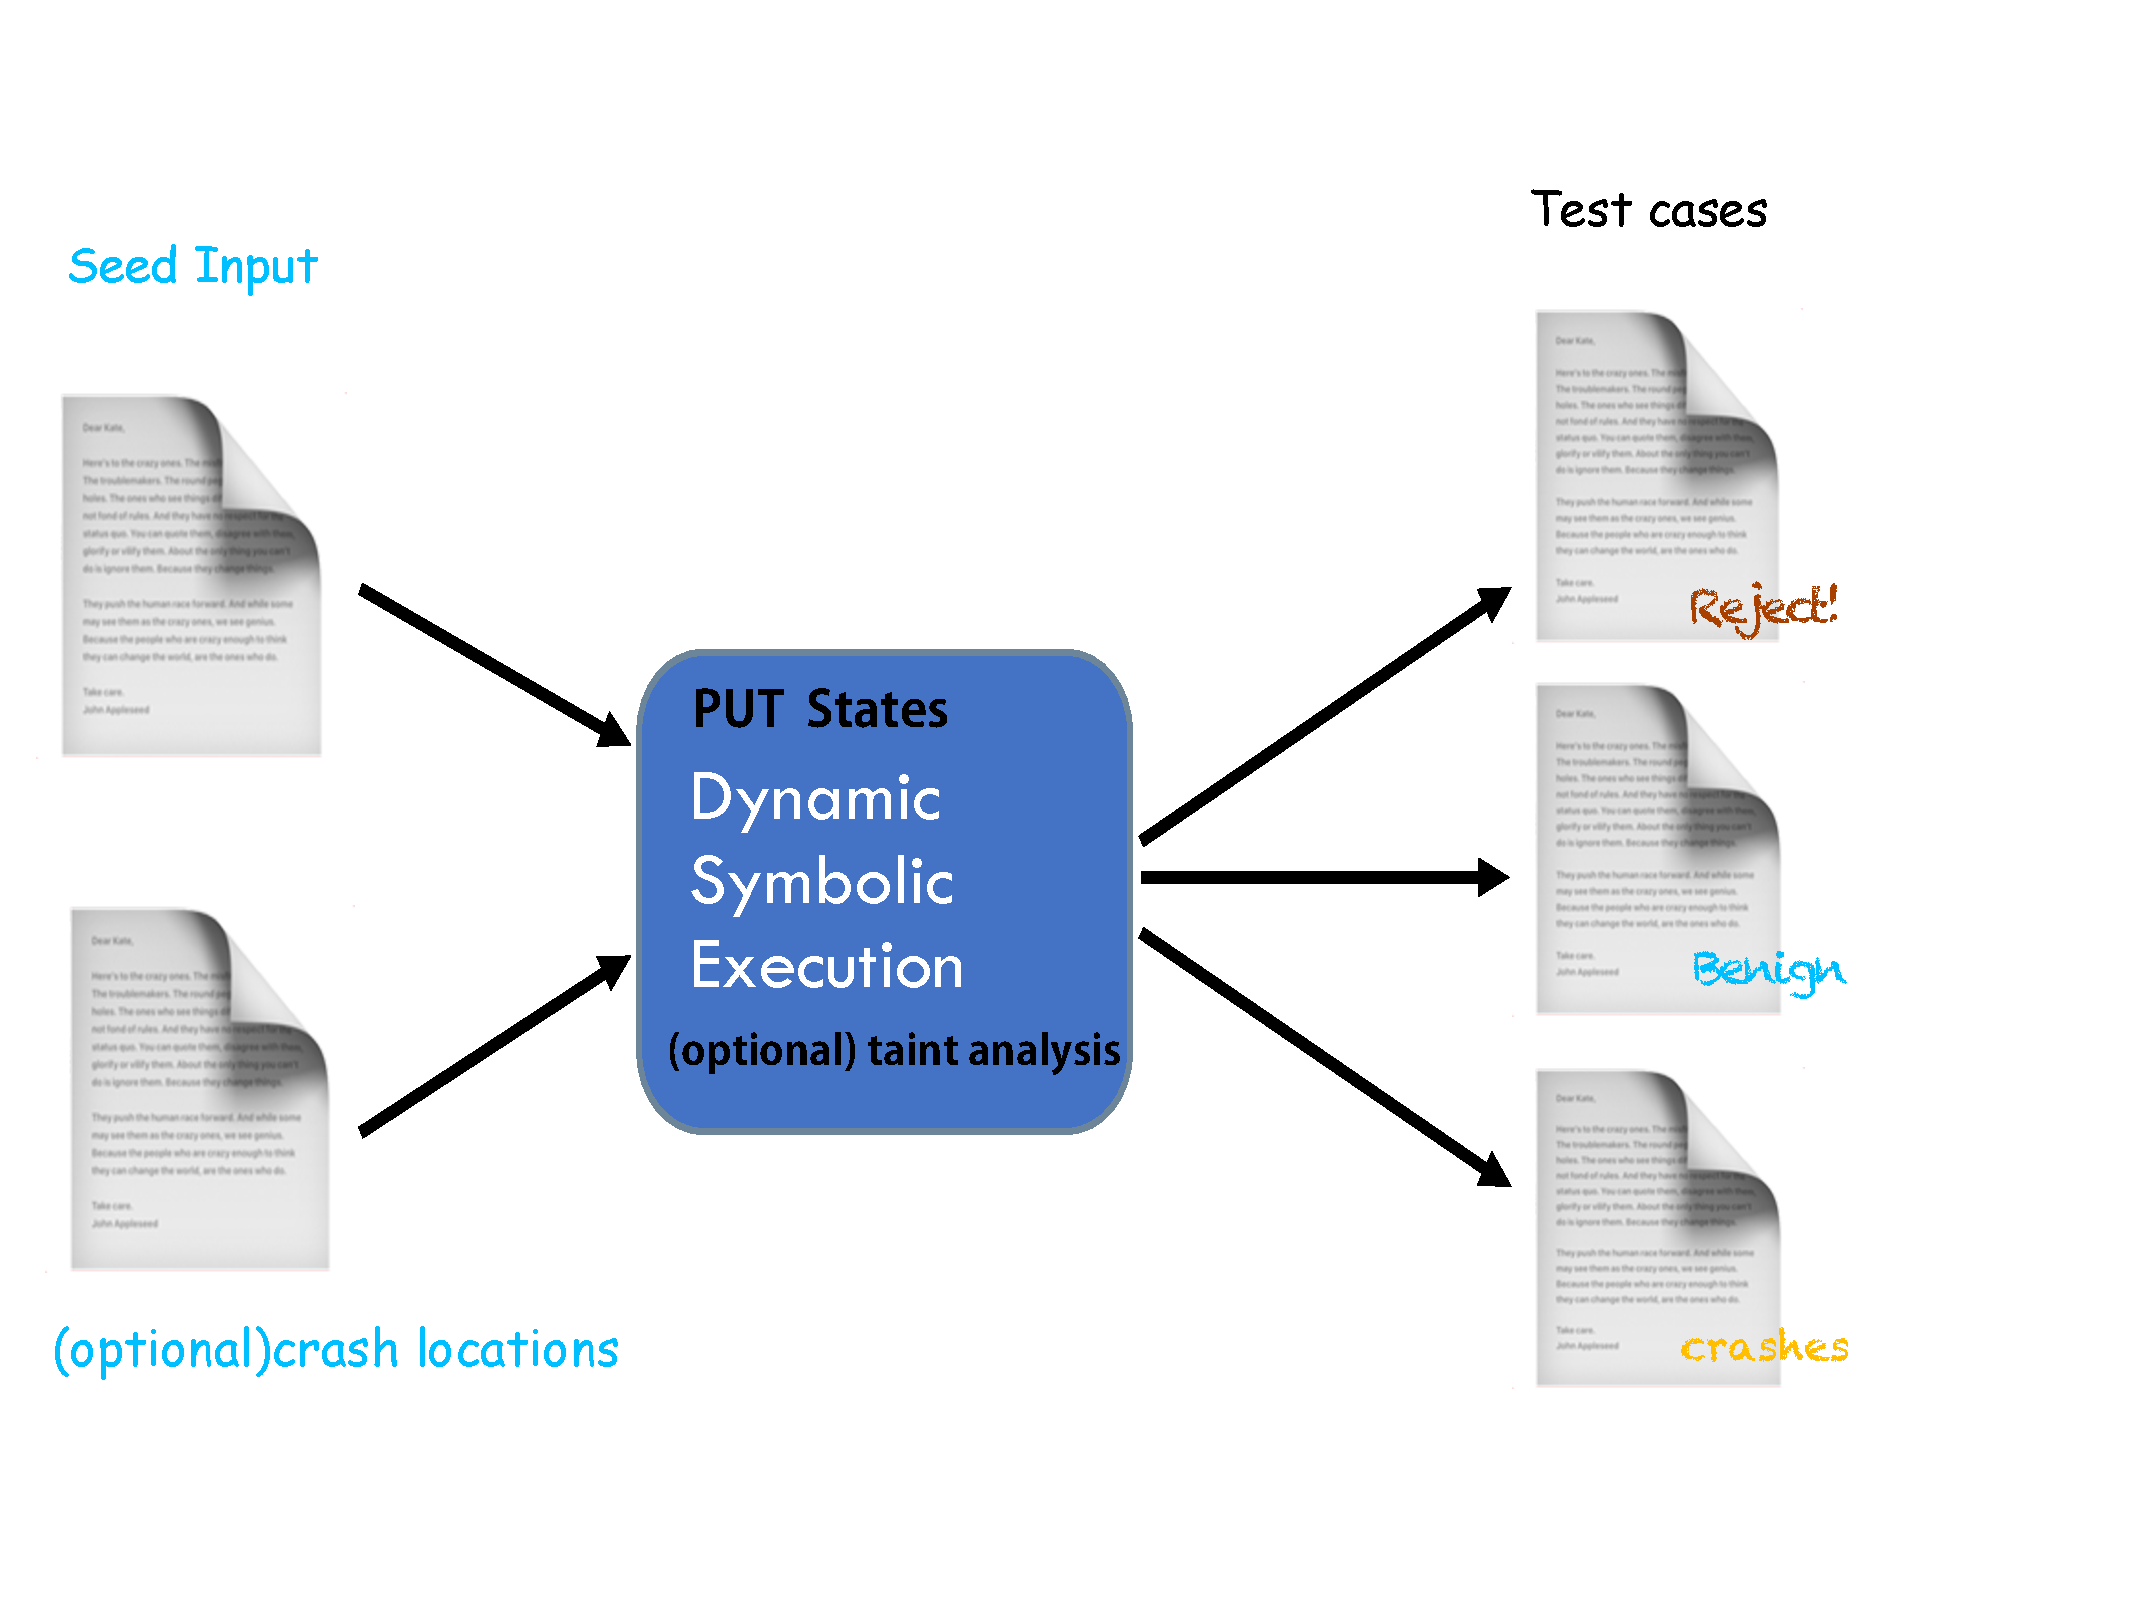
\includegraphics[width=6.0cm]{pic/whitebox.pdf}} 
        \end{picture} 
    }
    \only<4>{
        \begin{itemize}  
        \item \structure {White-box Fuzzing}
          \\ \textbf{Defination:} techniques that generates test cases by analyzing the internals of the PUT and the information gathered 
          when executing the PUT\cite{manes2019art}.
          \\ - Requires heavy-weight \alert {program analysis} and constraint solving. 
        \end{itemize}
        \begin{picture}(320,250) 
        \put(-15,110){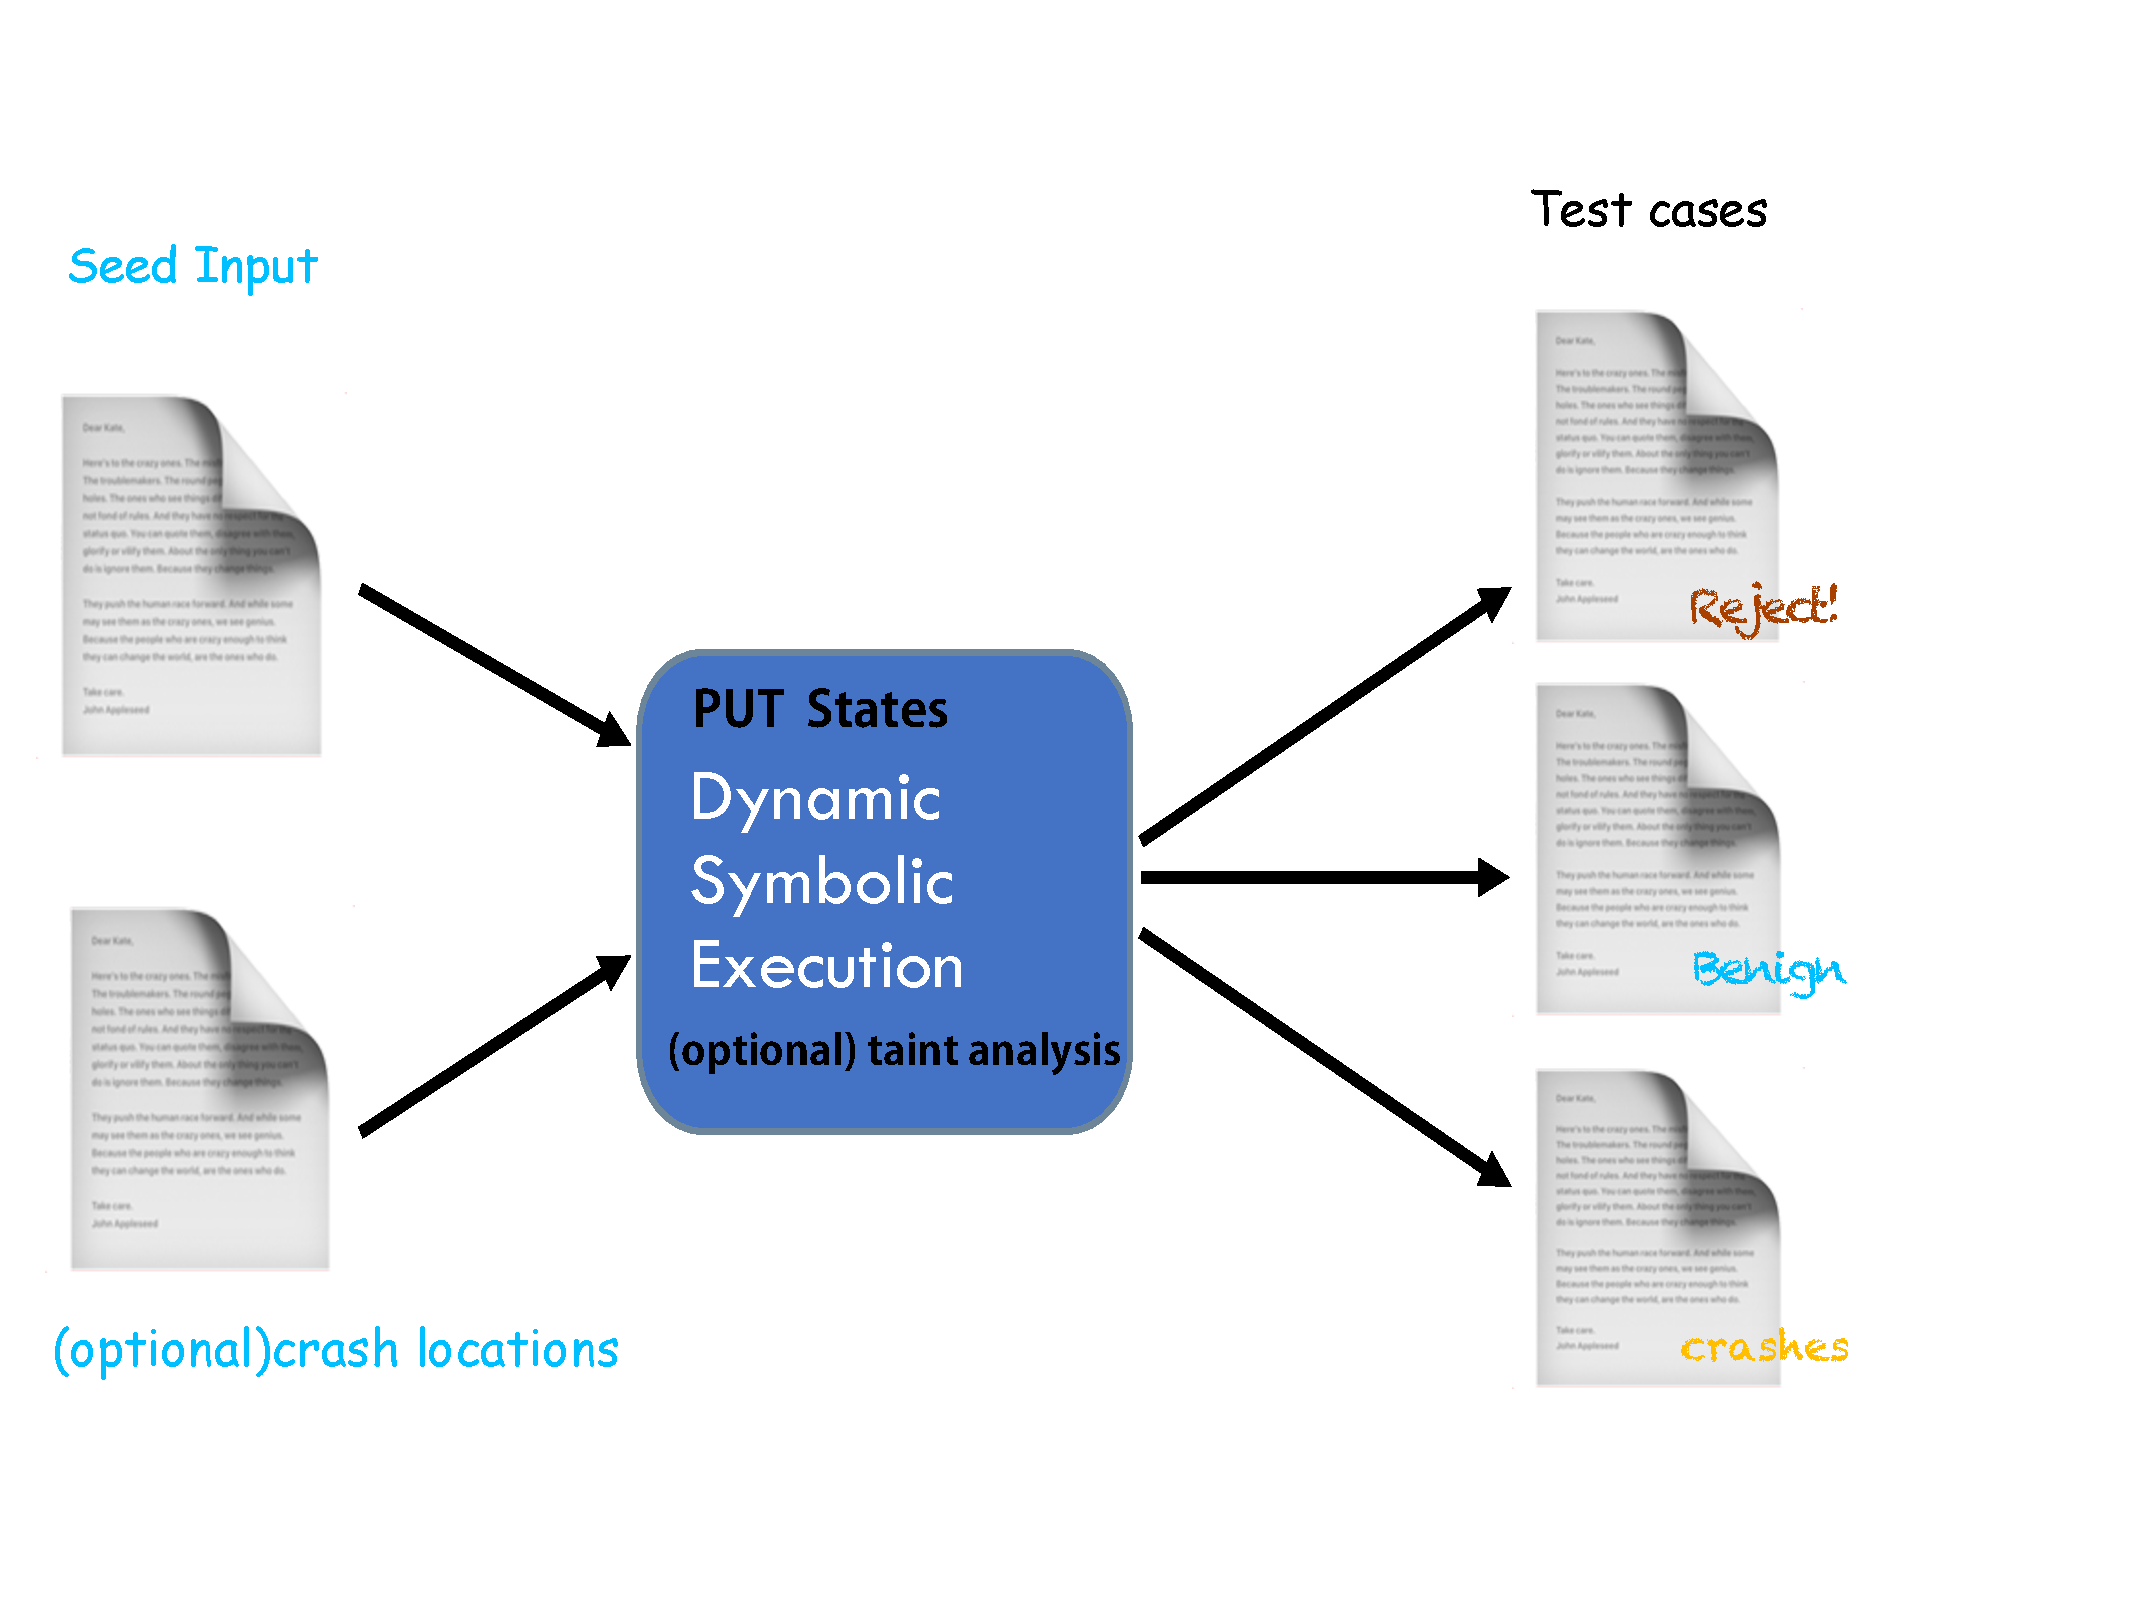
\includegraphics[width=8.0cm]{pic/whitebox.pdf}}
        \put(200,210){
            \begin{minipage}[t]{0.40\linewidth}
            {
                \footnotesize{
                    \begin{itemize}  
                        \item  You have the view of the PUT state(CFG,CG)
                        \item  Heavy-weight Program analysis (effective but not \alert {efficient}!)
                    \end{itemize} 
                }
            }
            \end{minipage}
        }
    \end{picture} 
    }
    \only<5>{
        \begin{itemize}  
        \item \structure {Grey-box Fuzzing}
          \\ \textbf{Defination:} techniques that can obtain \textsl{some} information internal to the PUT and/or its executions to generates test cases\cite{manes2019art}.
          \\ - Uses only lightweight instrumentation to glean some program structure
          \\ - And coverage \alert{feedback} 
        \end{itemize} 
        \begin{figure}[htbp]
            \begin{center}
                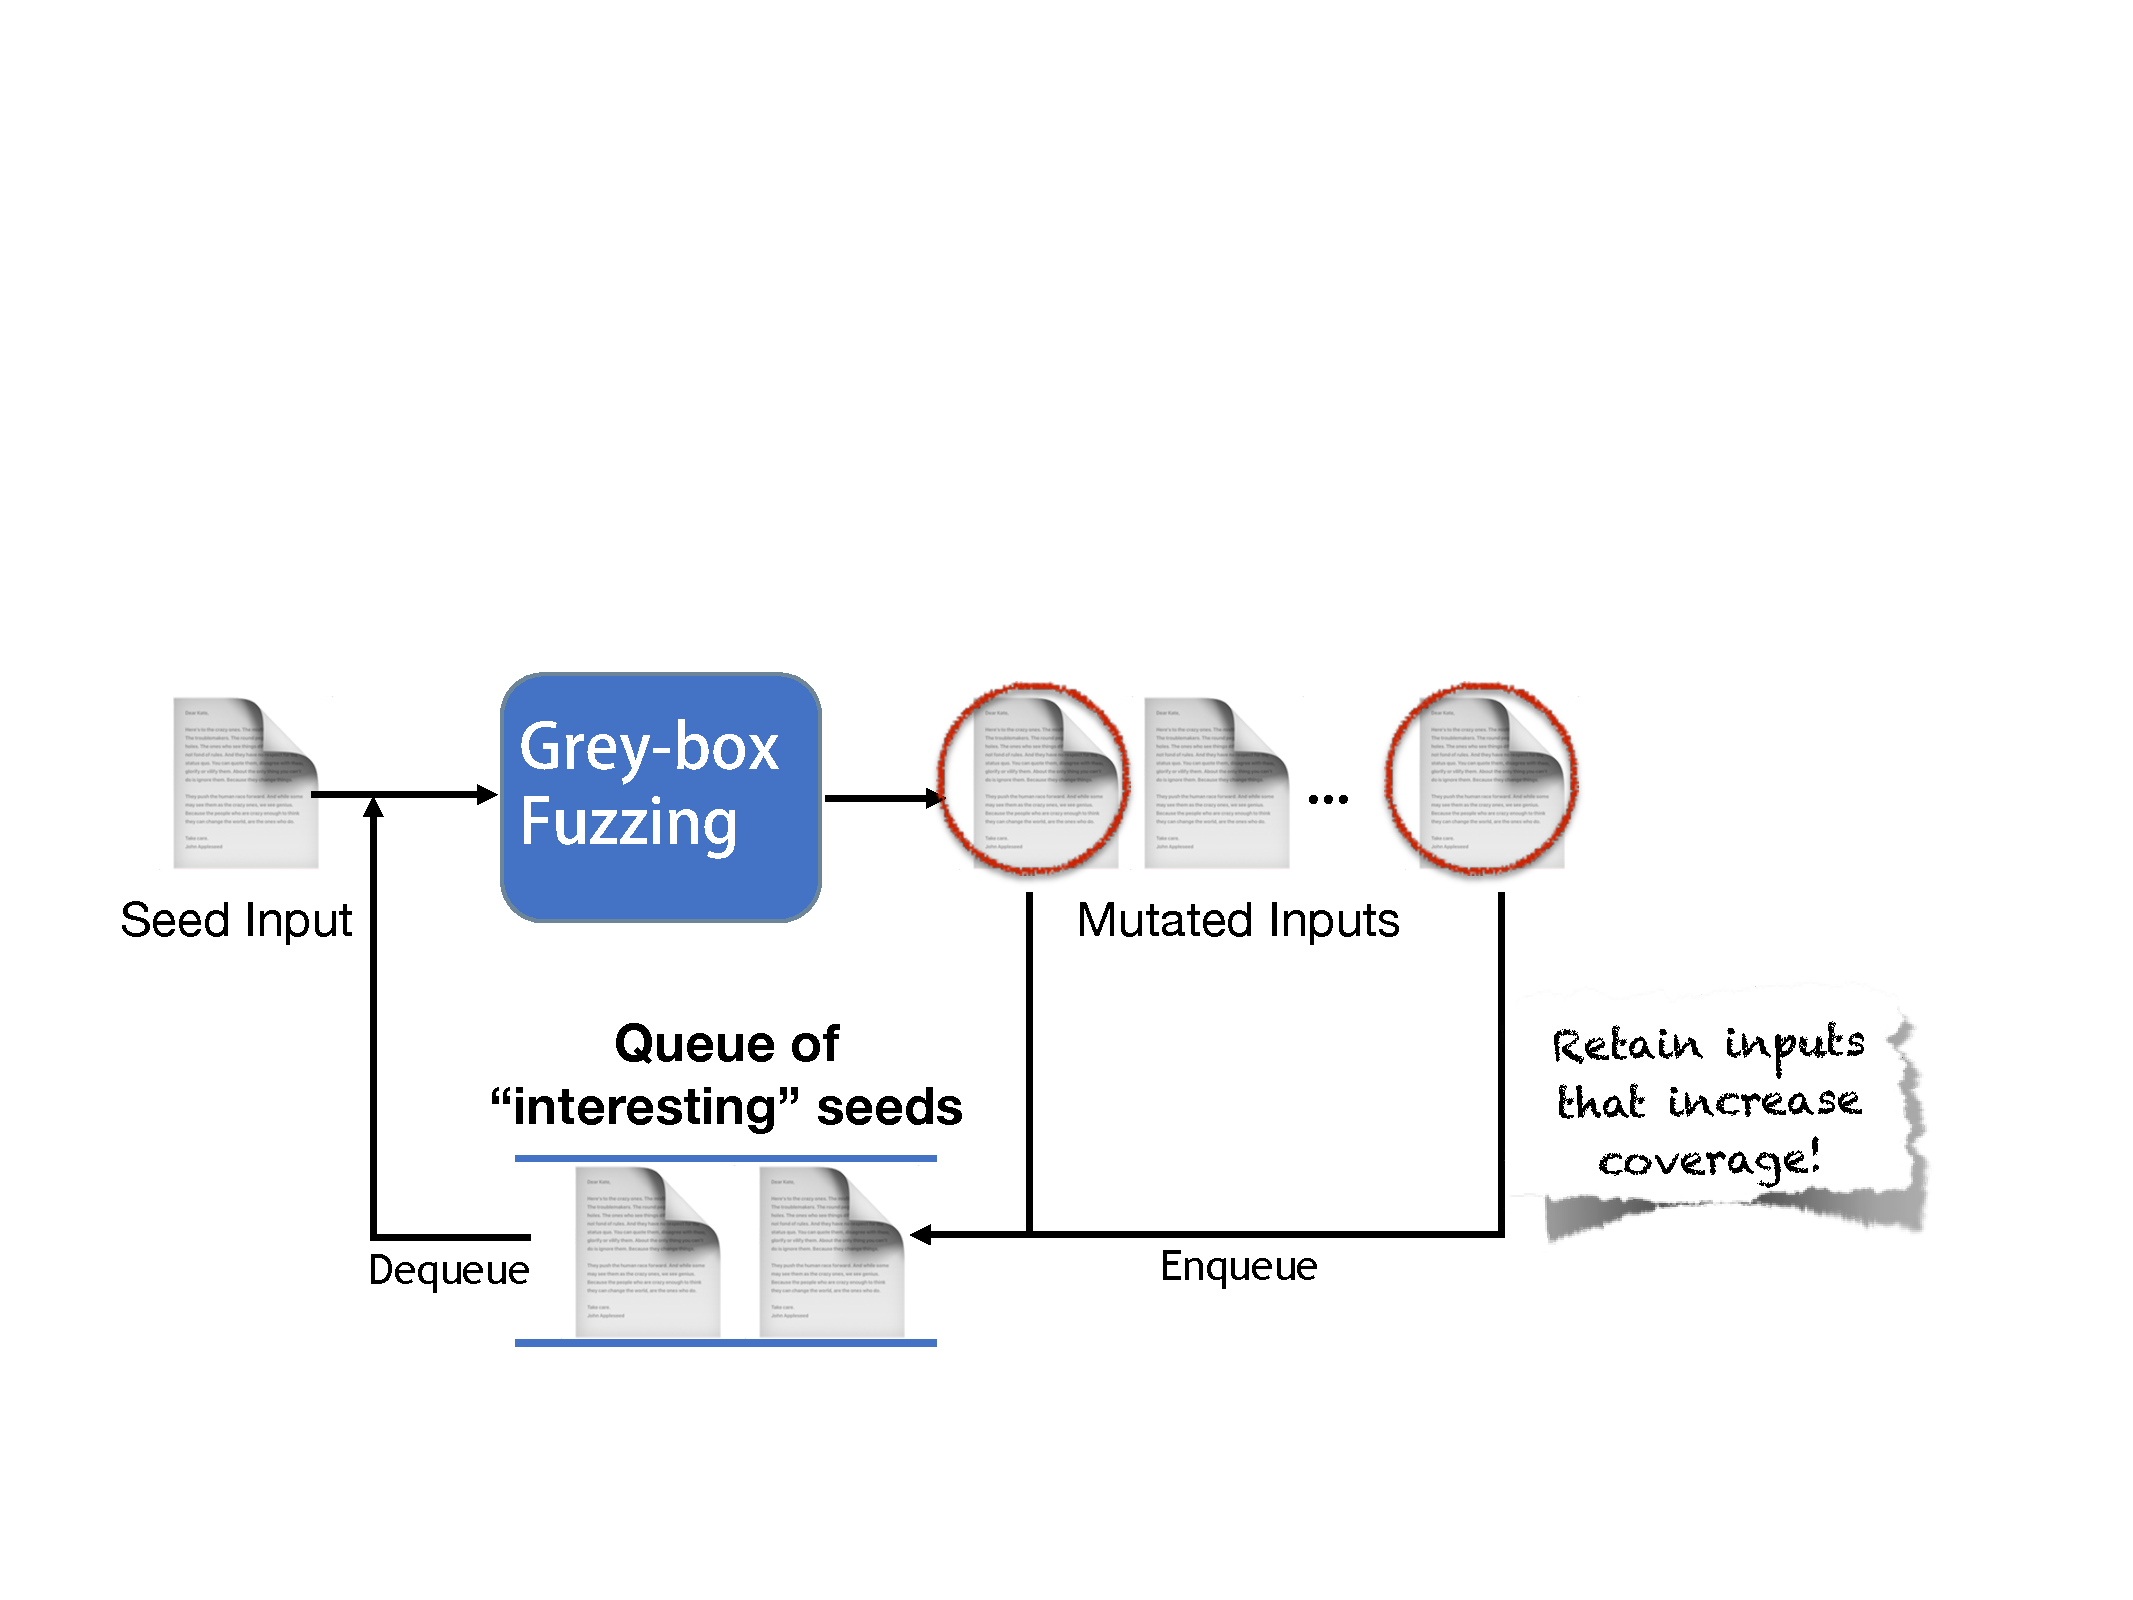
\includegraphics[width=10.0cm]{pic/greybox.pdf}
            \end{center}
        \end{figure} 
    }
    \only<6>{
        \textbf{ \structure {Grey-box Fuzzing} is frequently used}
        \begin{itemize}  
            \item \textbf{\textcolor{deepgreen}{State-of-the-art}} in automated vulnerability detection
            \item \textbf{\textcolor{deepgreen}{Extremely efficient}} coverage-based input generation 
                \begin{itemize}
                    \item[-]   All program analysis before/at \textcolor{deepred}{instrumentation time}.
                    \item[-]   Start with a seed corpus, choose a seed file, fuzz it.
                    \item[-]   Add to corpus only if new input increases coverage.
                \end{itemize} 
        \end{itemize}
    } 
\end{frame}

\begin{frame}{Why Directed Grey-box Fuzzing ?}
    \only<1>{
    \textbf{ \structure {Directed Fuzzing} has many applications} 
    \begin{itemize}  
        \item \textbf{\textcolor{deepgreen}{Patch Testing}}: reach changed statements
        \item \textbf{\textcolor{deepgreen}{Crash Reproduction}}: exercise stack trace
        \item \textbf{\textcolor{deepgreen}{SA Report Verification}}: reach “dangerous” location
        \item \textbf{\textcolor{deepgreen}{Information Flow Detection}}: exercise source-sink pairs
    \end{itemize} 
    }
    \only<2>{
        \textbf{\structure {Directed Fuzzing}}
        \begin{itemize}  
            \item \textbf{\textcolor{deepgreen}{Goal}:reach a specific \textcolor{deepred}{target}}
            \begin{itemize}
                \item[--]  \textbf{\alert{Target Locations}}: the line number in the source code or the virtual memory address at the binary level\cite{wang2022}.
                \item[--]  \textbf{Target Bugs}: use-after-free vulnerabilities, etc.
            \end{itemize} 
            \begin{minipage}[t]{0.7\linewidth}
            \vspace{0pt} 
            \item \textbf{\textcolor{deepgreen}{DSE}:classical \textcolor{deepred}{constraint satisfaction problem}}
            \begin{itemize}
                \item[--]  uses program analysis and constraint solving to generate inputs that systematically 
                         and effectively explore the state space of feasible paths\cite{ma2011directed}.
                \item[--]  \alert{\textbf{Program analysis}} to identify \textcolor{deepblue}{\textbf{program paths}} that reach given program locations.
                \item[--]  \alert{\textbf{Symbolic Execution}} to derive \textcolor{deepblue}{\textbf{path conditions}} for any of the identified paths.
                \item[--] \alert{\textbf{Constraint Solving}} to find an input 
            \end{itemize}  
            \end{minipage}
            \begin{minipage}[t]{0.28\linewidth}
                \vspace{0pt}
                \centering 
                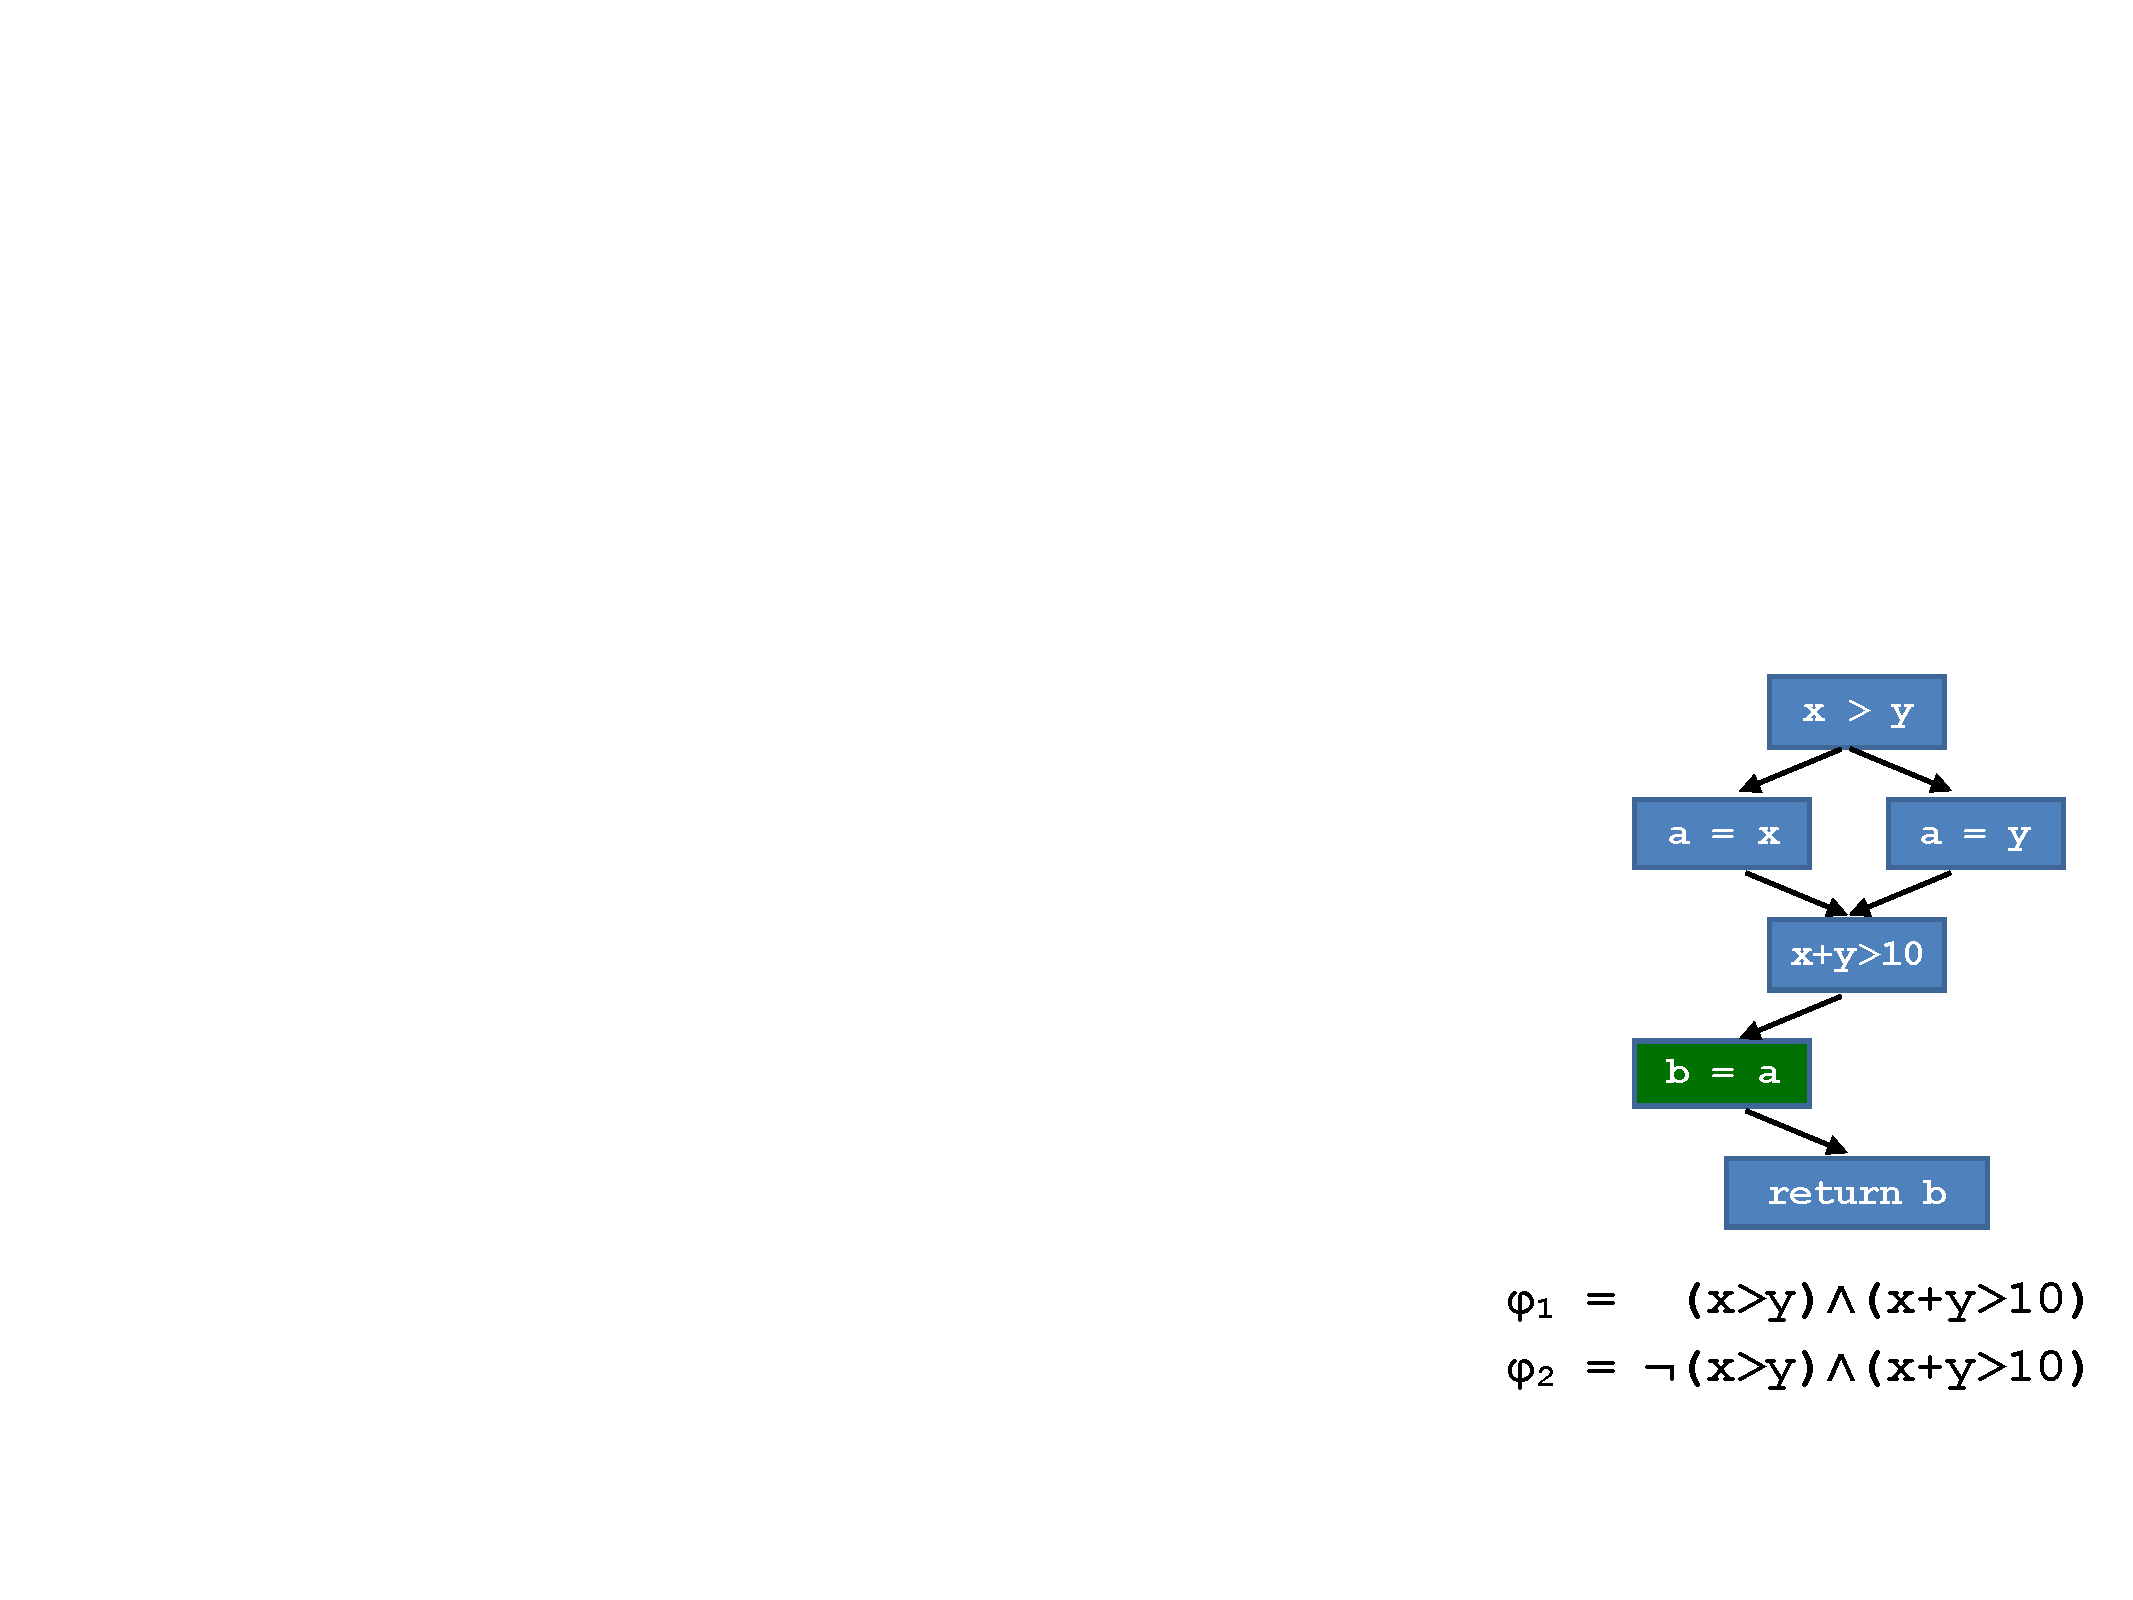
\includegraphics[width=3.0cm]{pic/dse.pdf} 
            \end{minipage} 
        \end{itemize} 
    }
    \only<3>{
        \textbf{\Large{
            \begin{itemize}  
                \item Effectiveness comes at the cost of \alert {efficiency}
                \item \alert {Heavy-weight} program analysis
            \end{itemize}
        }}
    }
\end{frame}


\subsection{Research Status}
\begin{frame}
    \structure {Genealogy tracing significant fuzzers’ lineage}\footnote{paper\cite{manes2019art}-Figure1}
    \begin{figure}[htbp]
        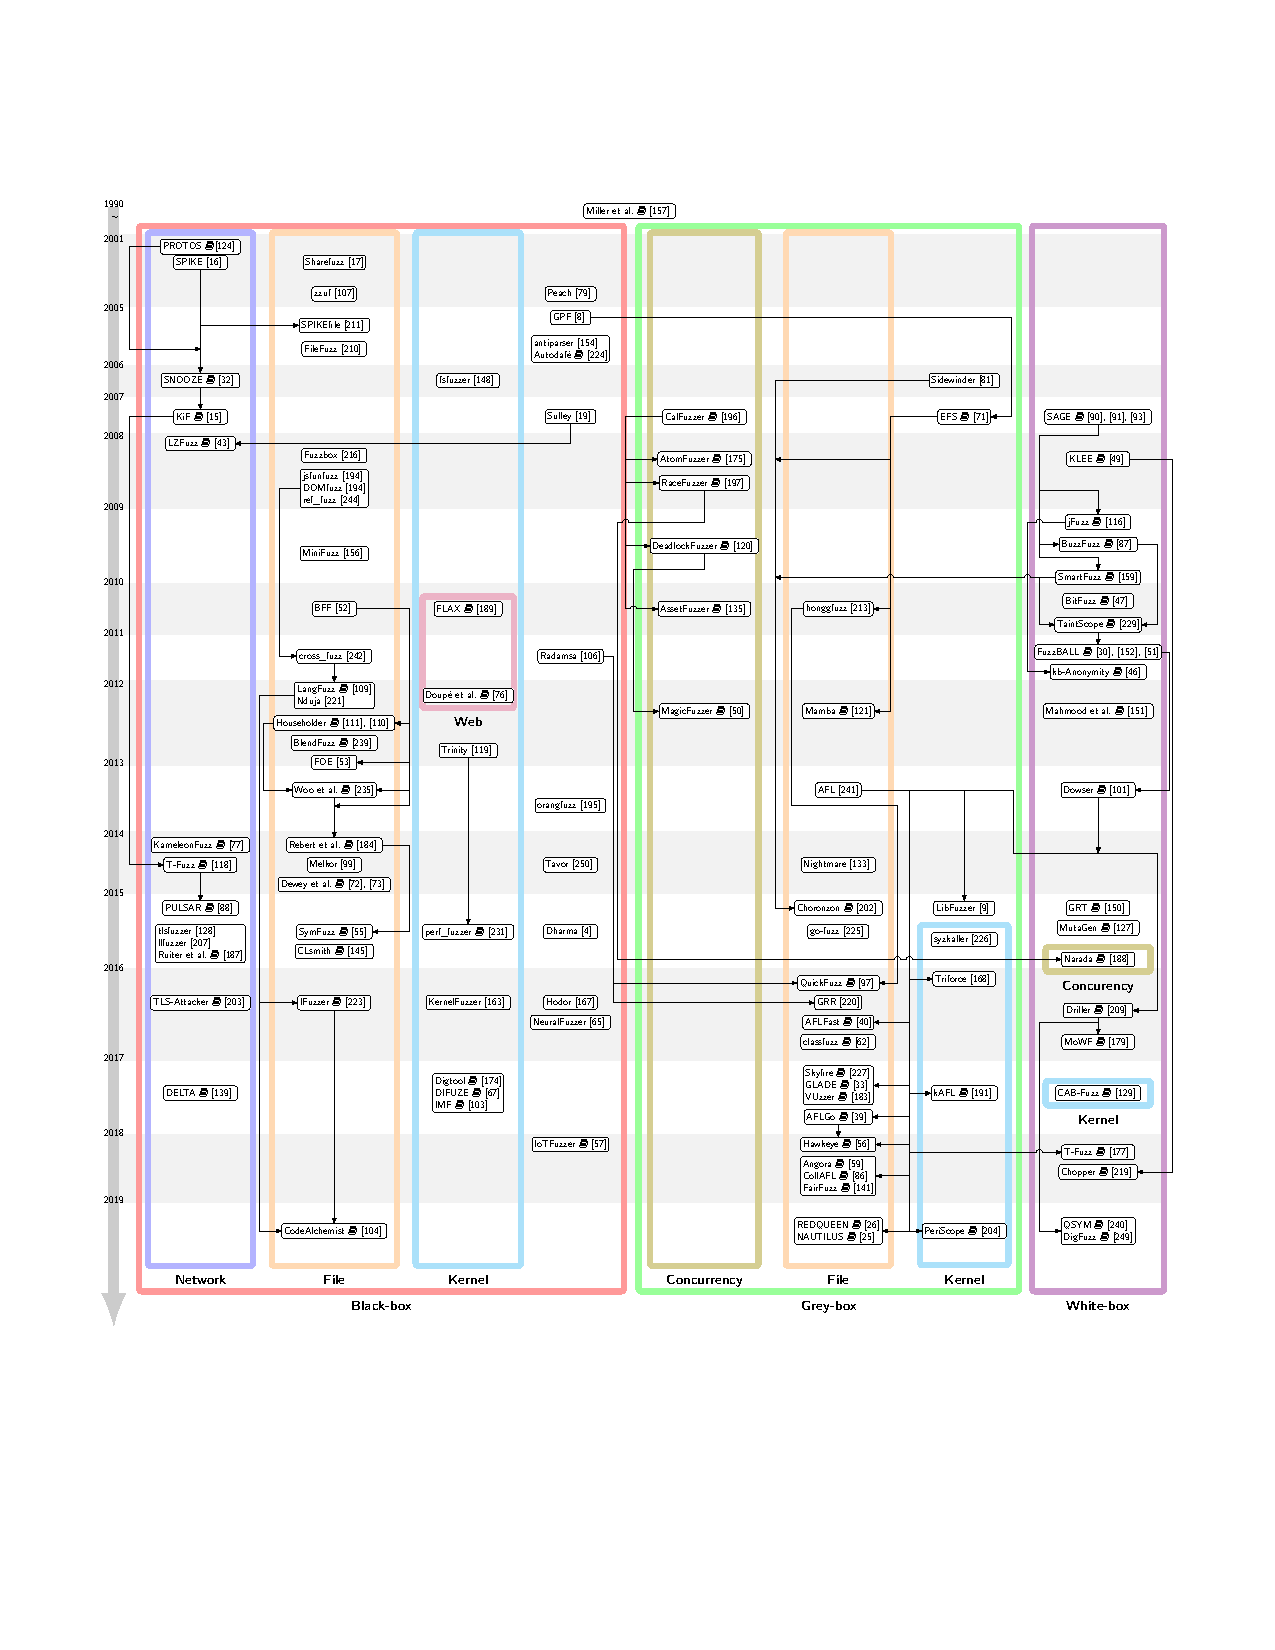
\includegraphics[width=7.0cm]{pic/gen.pdf}
    \end{figure}
\end{frame}

\begin{frame}
    \textbf{ \structure {Representative Work}}
        \begin{itemize}  
            \item \textbf{\textcolor{deepgreen}{AFLGo(2017)}}\cite{bohmeDGF2017}
            \item \textbf{\textcolor{deepgreen}{Hawkeye(2018)}}\cite{chenHawkeye2018} 
        \end{itemize} 
\end{frame}

\section{Theory}
\subsection{AFLGo}
\begin{frame}{OverView}
    \only<1>{
        \textbf{ \structure {Directed Fuzzing} as \textcolor{deepgreen}{optimisation problem!}}
        \begin{itemize} 
            \item \textbf{Instrumentation Time}
                \begin{enumerate}
                    \item Extract \textbf{\textcolor{deepred}{call graph}} (CG) and \textbf{\textcolor{deepred}{control-flow graphs}} (CFGs).
                    \item For each \textbf{\textcolor{deepred}{BB}}, compute \textbf{\textcolor{deepred}{distance}} to target locations.
                    \item Instrument program to \textbf{\textcolor{deepred}{aggregate distance values}}.
                \end{enumerate} 
            \item \textbf{Runtime}
                \begin{enumerate}
                    \item collect coverage and distance \textbf{\textcolor{deepred}{information}}, and
                    \item decide \textbf{\textcolor{deepred}{how long to be fuzzed}} based on distance.
                    \begin{itemize}
                        \item[--] If input is \textbf{\textcolor{deepgreen}{closer}} to the targets, it is fuzzed for \textbf{\textcolor{deepgreen}{longer}}.
                        \item[--] If input is \textbf{\textcolor{deepred}{further away}} from the targets, it is fuzzed for \textbf{\textcolor{deepred}{shorter}}.
                    \end{itemize}  
                \end{enumerate}  
        \end{itemize}  
    }
    \only<2>{
        \textbf{ \structure {AFLGo Architecture}}
        \begin{figure}[htbp]
            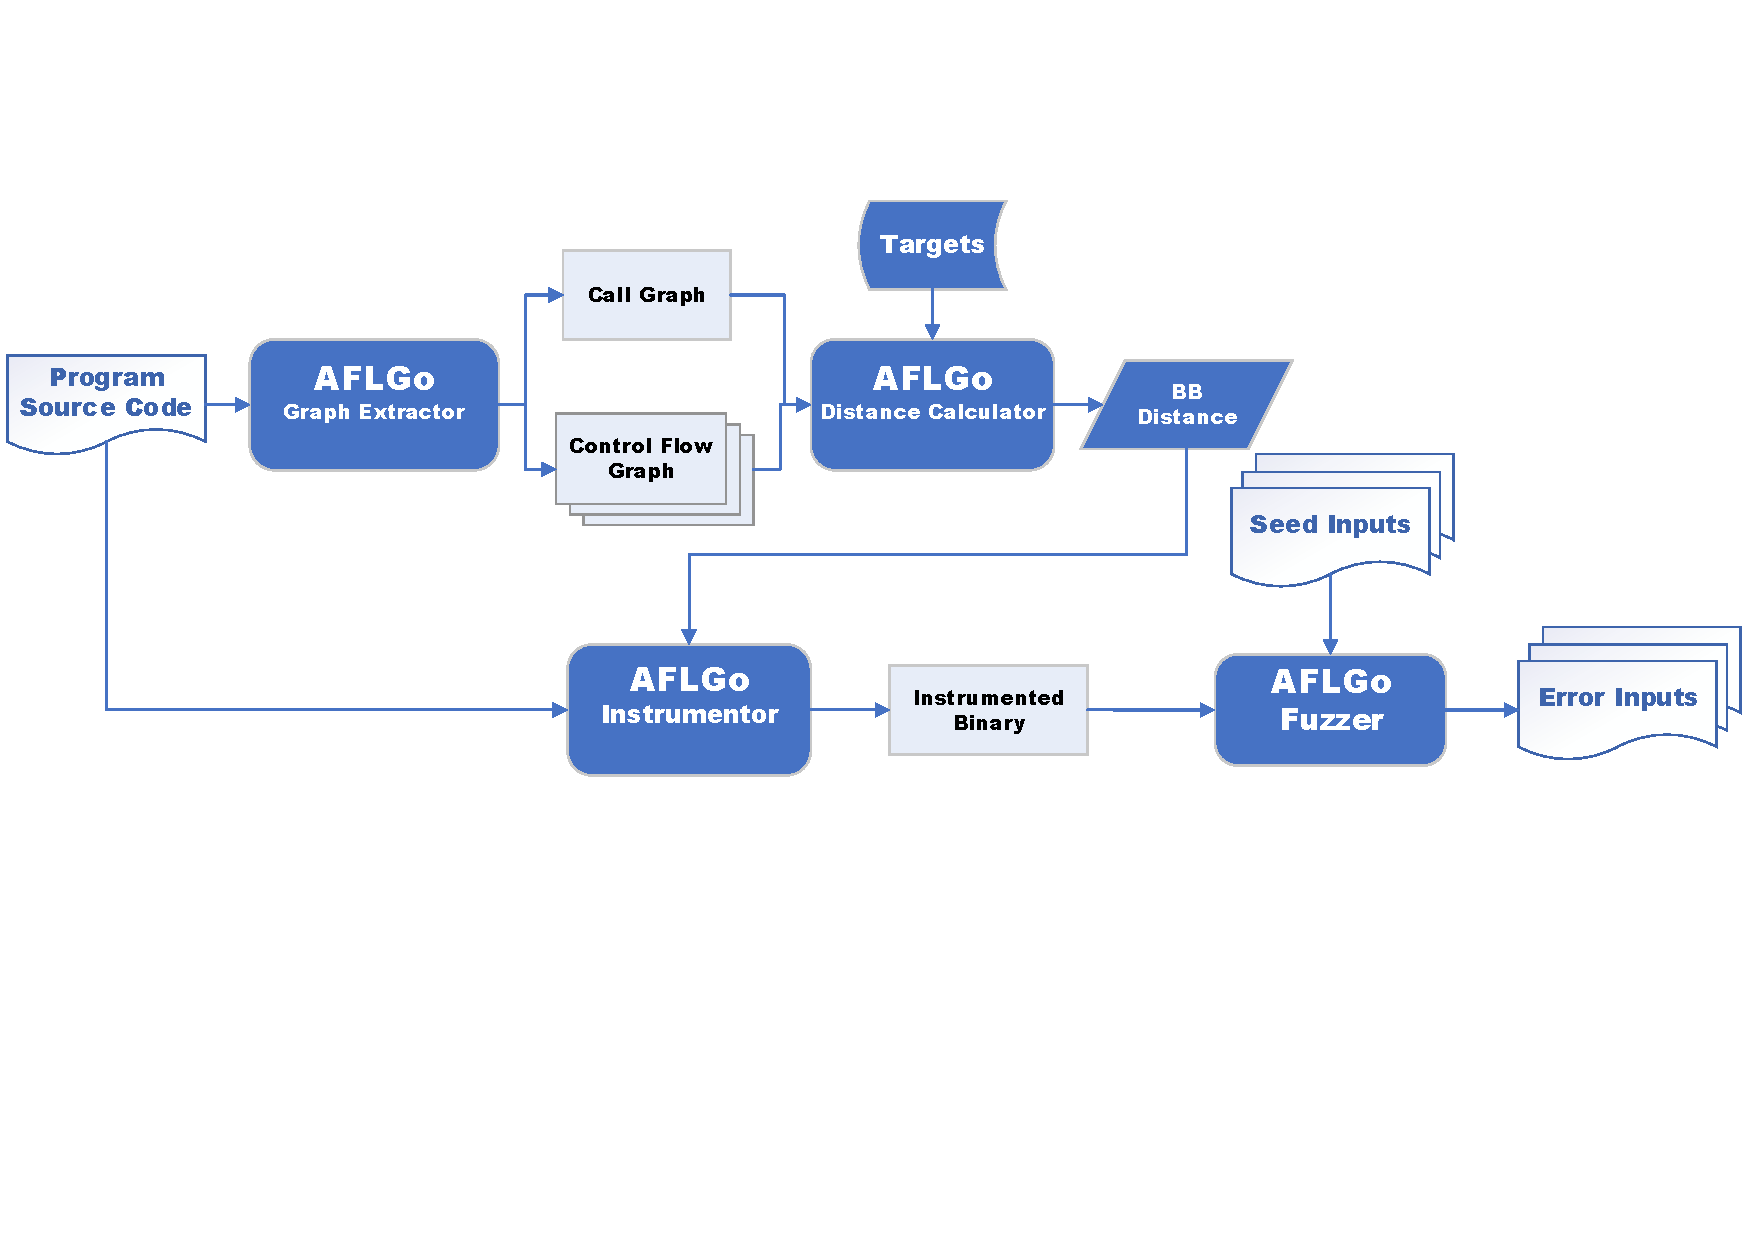
\includegraphics[width=11.5cm]{pic/AFLGo.pdf}
        \end{figure}
    } 
\end{frame}

\begin{frame}{Algorithm}
        \begin{block}{Directed Grey-box Fuzzing}
            \begin{algorithm}[H]
                \footnotesize
                \DontPrintSemicolon
                \SetKwSty{algokeywordsty}
                \SetFuncSty{algofuncsty}
                \SetDataSty{algodatasty}
                \SetArgSty{algoargsty}
                \SetCommentSty{algocmtsty}
                \SetKw{break}{break}
                \SetKw{not}{not}
                \SetKwFunction{graphextractor}{\textsc{GraphExt}}
                \SetKwFunction{bbdistance}{\textsc{DisCalcu}}  
                \SetKwFunction{select}{\textsc{Dequeue}}
                \SetKwFunction{assinenergy}{\textsc{AssinEnergy}}
                \SetKwFunction{mutation}{\textsc{Mutation}}
                \SetKwFunction{execution}{\textsc{Execution}}
                \SetKwFunction{IsIntersting}{\textsc{IsIntersting}}
                \SetKwFunction{evaluateseed}{\textsc{SeedDis}}
                \SetKwFunction{sortinsert}{Enqueue}
                % \SetKwData{crashseeds}{$\seeds_{\text{\emoji{boom}}}$}
                \SetKwData{crashseeds}{$\seeds^\prime$} 
                \SetKwData{seedqueue}{$\textit{SeedQueue}$}  
                \SetKwData{Graph}{$\textit{Graphs}$}  
                \SetKwData{BBdis}{$\textit{BBdistance}$} 
                \SetKwData{newseed}{$\seed^\prime$}   
                \SetKwData{energy}{$\textit{e}$}
                \SetKwData{trace}{$\textit{trace}$} 
                \SetKwData{distance}{$\textit{distance}$}   
                \KwIn{\seeds\tcp{a finite set of seeds}}
                \KwIn{\targets\tcp{a finite set of targer sits}} 
                \KwOut{\crashseeds \tcp{a finite set of buggy seeds}}
                $\crashseeds\gets \varnothing$\; 
                $\seedqueue \gets \seeds$\;
                \Graph $\gets \graphextractor{\sourcecode}$\;
                \BBdis $\gets \bbdistance{\targets,\Graph}$\;
                \While {$!siganl \land \currtime < \timeout$}{
                  \seed$\gets \select{\seedqueue}$\;
                  $\trace \gets \execution{\seed}$\; 
                  $\distance \gets \evaluateseed{\trace, \BBdis} $\;
                  \energy $\gets \assinenergy{\seed, \currtime, \distance}$\;
                   \For{$\textit{i}\gets 1$ \KwTo $\energy$}
                   {
                    $\newseed \gets \mutation{\seed}$\;      
                    \lIf{\newseed crashes}{$\crashseeds \gets \crashseeds \cup \newseed $}
                    \lIf{\IsIntersting{\newseed}}{    
                        $\sortinsert{\newseed,\seedqueue} $ 
                    }
                   }
                }
                \Return{\crashseeds}\;
            \end{algorithm} 
        \end{block}
\end{frame}

\begin{frame}{Instrumentation}
    \only<1>{
        \begin{algorithm}[H]
            \footnotesize
            \DontPrintSemicolon
            \SetKwSty{algokeywordsty}
            \SetFuncSty{algofuncsty}
            \SetDataSty{algodatasty}
            \SetArgSty{algoargsty}
            \SetCommentSty{algocmtsty}
            \SetKw{break}{break}
            \SetKw{not}{not}
            \SetKwFunction{graphextractor}{\textsc{GraphExt}}
            \SetKwFunction{bbdistance}{\textsc{DisCalcu}}  
            \SetKwFunction{select}{\textsc{Dequeue}}
            \SetKwFunction{assinenergy}{\textsc{AssinEnergy}}
            \SetKwFunction{mutation}{\textsc{Mutation}}
            \SetKwFunction{execution}{\textsc{Execution}}
            \SetKwFunction{IsIntersting}{\textsc{IsIntersting}}
            \SetKwFunction{evaluateseed}{\textsc{SeedDis}}
            \SetKwFunction{sortinsert}{Enqueue}
            % \SetKwData{crashseeds}{$\seeds_{\text{\emoji{boom}}}$}
            \SetKwData{crashseeds}{$\seeds^\prime$} 
            \SetKwData{seedqueue}{$\textit{SeedQueue}$}  
            \SetKwData{Graph}{$\textit{Graphs}$}  
            \SetKwData{BBdis}{$\textit{BBdistance}$} 
            \SetKwData{newseed}{$\seed^\prime$}   
            \SetKwData{energy}{$\textit{e}$}
            \SetKwData{trace}{$\textit{trace}$} 
            \SetKwData{distance}{$\textit{distance}$}   
            \KwIn{\seeds\tcp{a finite set of seeds}}
            \KwIn{\targets\tcp{a finite set of targer sits}} 
            \KwOut{\crashseeds \tcp{a finite set of buggy seeds}}
            $\crashseeds\gets \varnothing$\; 
            $\seedqueue \gets \seeds$\;
            \HiLi\Graph $\gets \graphextractor{\sourcecode}$\;
            \HiLi\BBdis $\gets \bbdistance{\targets,\Graph}$\;
            \While {$!siganl \land \currtime < \timeout$}{
              \seed$\gets \select{\seedqueue}$\;
              $\trace \gets \execution{\seed}$\; 
              $\distance \gets \evaluateseed{\trace, \BBdis} $\;
              \energy $\gets \assinenergy{\seed, \currtime, \distance}$\;
               \For{$\textit{i}\gets 1$ \KwTo $\energy$}
               {
                $\newseed \gets \mutation{\seed}$\;      
                \lIf{\newseed crashes}{$\crashseeds \gets \crashseeds \cup \newseed $}
                \lIf{\IsIntersting{\newseed}}{    
                    $\sortinsert{\newseed,\seedqueue} $ 
                }
               }
            }
            \Return{\crashseeds}\;
        \end{algorithm} 
    }
    \only<2->{
        \begin{itemize}  
            \onslide<2-> \item \textbf{\structure {Function-level target distance\only<2>{\footnote{R(n,Tf ) is the set of all target functions that are reachable from n in CG}}}}:using call graph \textcolor{deepred}{(CG)}
            \onslide<5-> \item \textbf{\textcolor{deepgreen}{BB-level target distance
            \only<5>{\footnote{
                \begin{itemize}
                    \item [-] N (m) is the set of functions called by basic block m
                    \item [-] T is the set of basic blocks in control-flow graph
                \end{itemize}
            }}}}:using control-flow graphs \textcolor{deepred}{(CFG)} 
        \end{itemize} 
        \onslide<2-> 
        \begin{minipage}[t]{0.7\linewidth}
        \vspace{0pt} 
        \only<2>{
                $$ d_f(n,T_f)=\left\{ \begin{aligned}
                         &\text{undefined} , &\text{if } R(n,T_f)=\varnothing \\
                        [&\sum\limits_{t_f\in R(n,T_f)} d_f(n,t_f)^{-1}]^{-1} , &\text{otherwise} 
                    \end{aligned}
                    \right.$$
        }
        \only<5>{
            \small
            $$ d_b(m,T_b)=\left\{ \begin{aligned}
                &0 ,&\text{if } m \in T_b \\
                &c \cdot \min \limits_{n\in N(m)}(d_f(n,T_f)) , &\text{if } m \in T \\
               [&\sum\limits_{t\in T} (d_b(m,t)+d_b(t,T_b))^{-1}]^{-1} , &\text{otherwise} 
           \end{aligned}
           \right.$$ 
        }
        \only<3-4>{
            \begin{enumerate}
               \item  Identify\textbf{ target functions} in CG
                \only<4>{ \item  For each \textbf{\textcolor{deepblue}{function}}, compute the \textbf{\alert{harmonic mean}} of the \textbf{\textcolor{deepred}{length of the shortest path}} to targets}
            \end{enumerate}
        }
        \only<6-9>{
            \begin{enumerate}
                \item  Identify\textbf{ target BBs} and assign distance 0 \\\only<6>{(none in function b)}
                \only<7-9>{\item  Identify BBs that \textbf{\textcolor{deepblue}{call function}} and assign \textbf{\textcolor{deepred}{10*FLTD}}}
                \only<8-9>{\item  For each BB, compute harmonic mean of (length of shortest path to any function-calling BB + 10*FLTD).} 
            \end{enumerate}
        }
        \only<4>{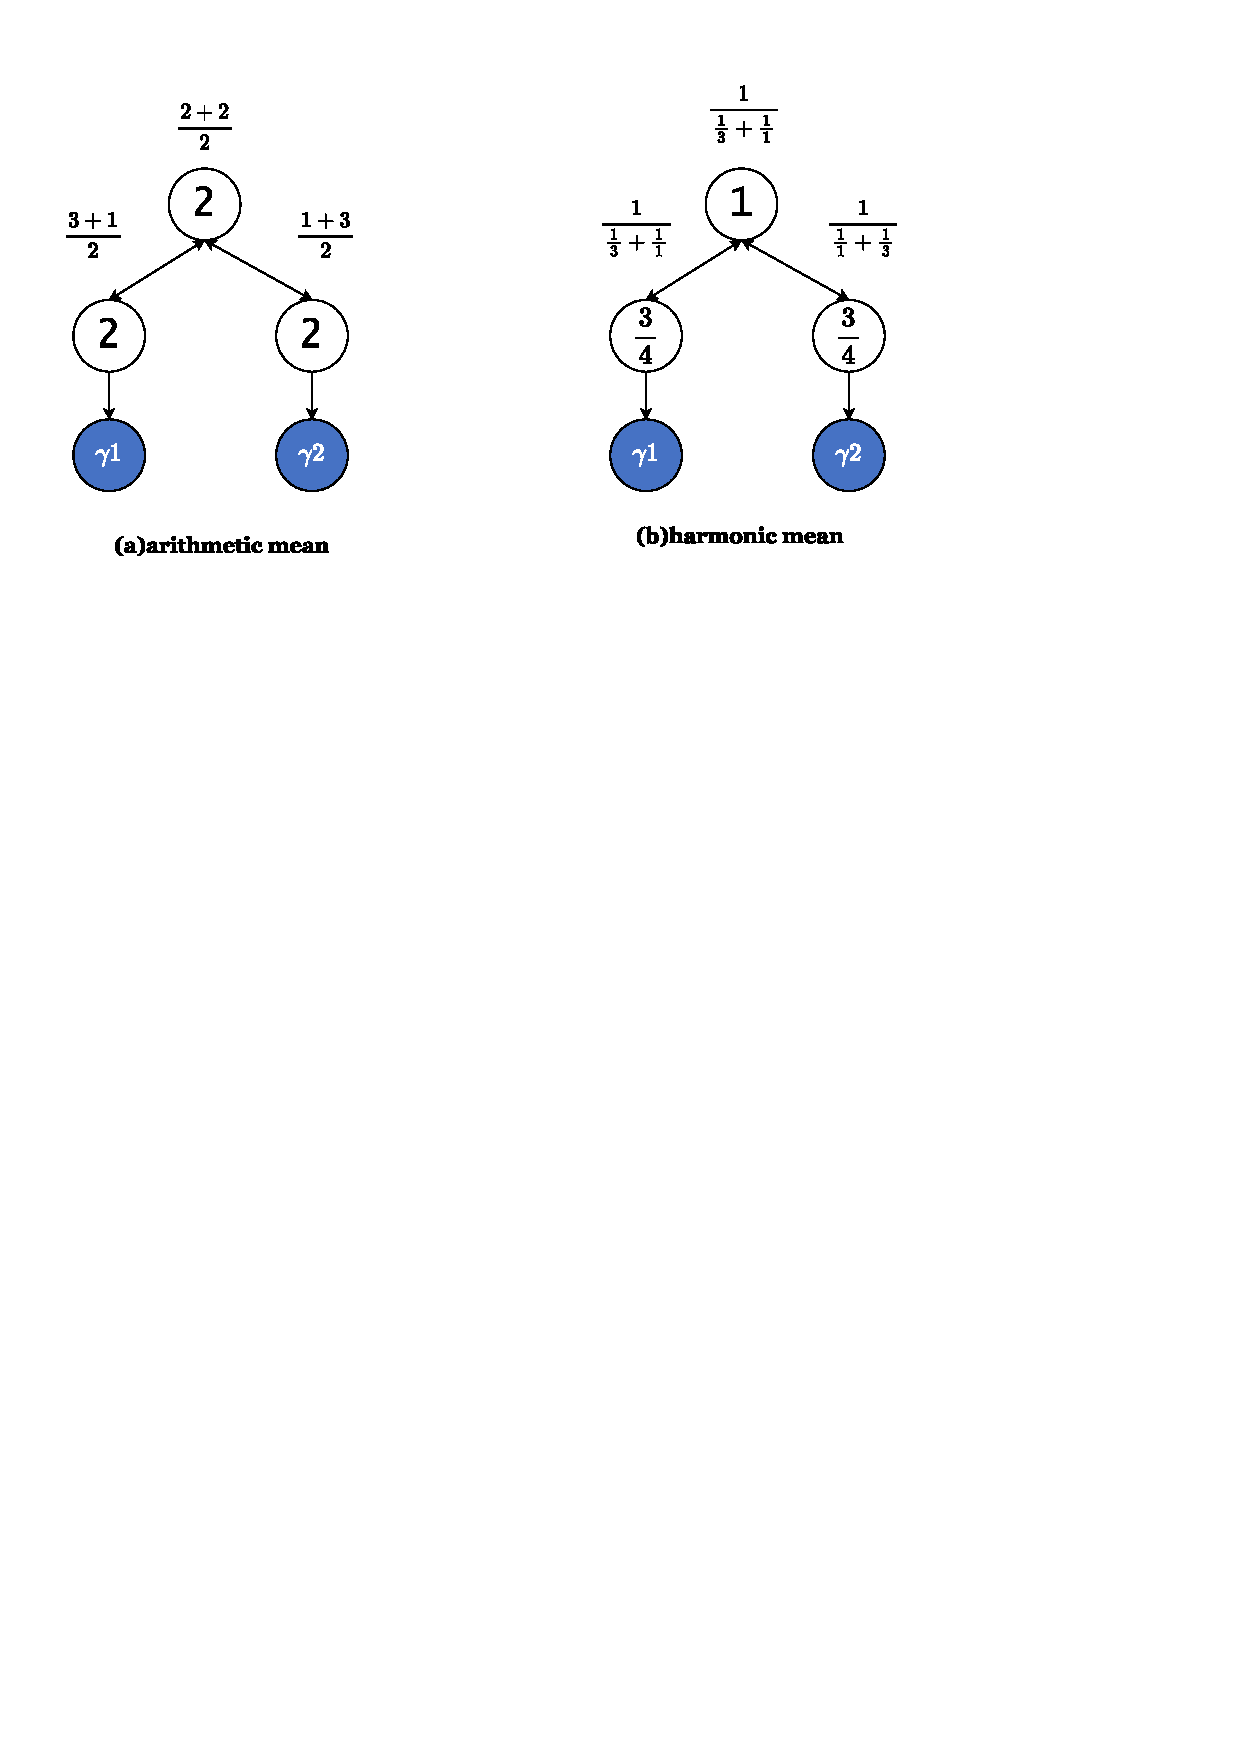
\includegraphics[width=6.0cm]{pic/diff.pdf} } 
        \only<7>{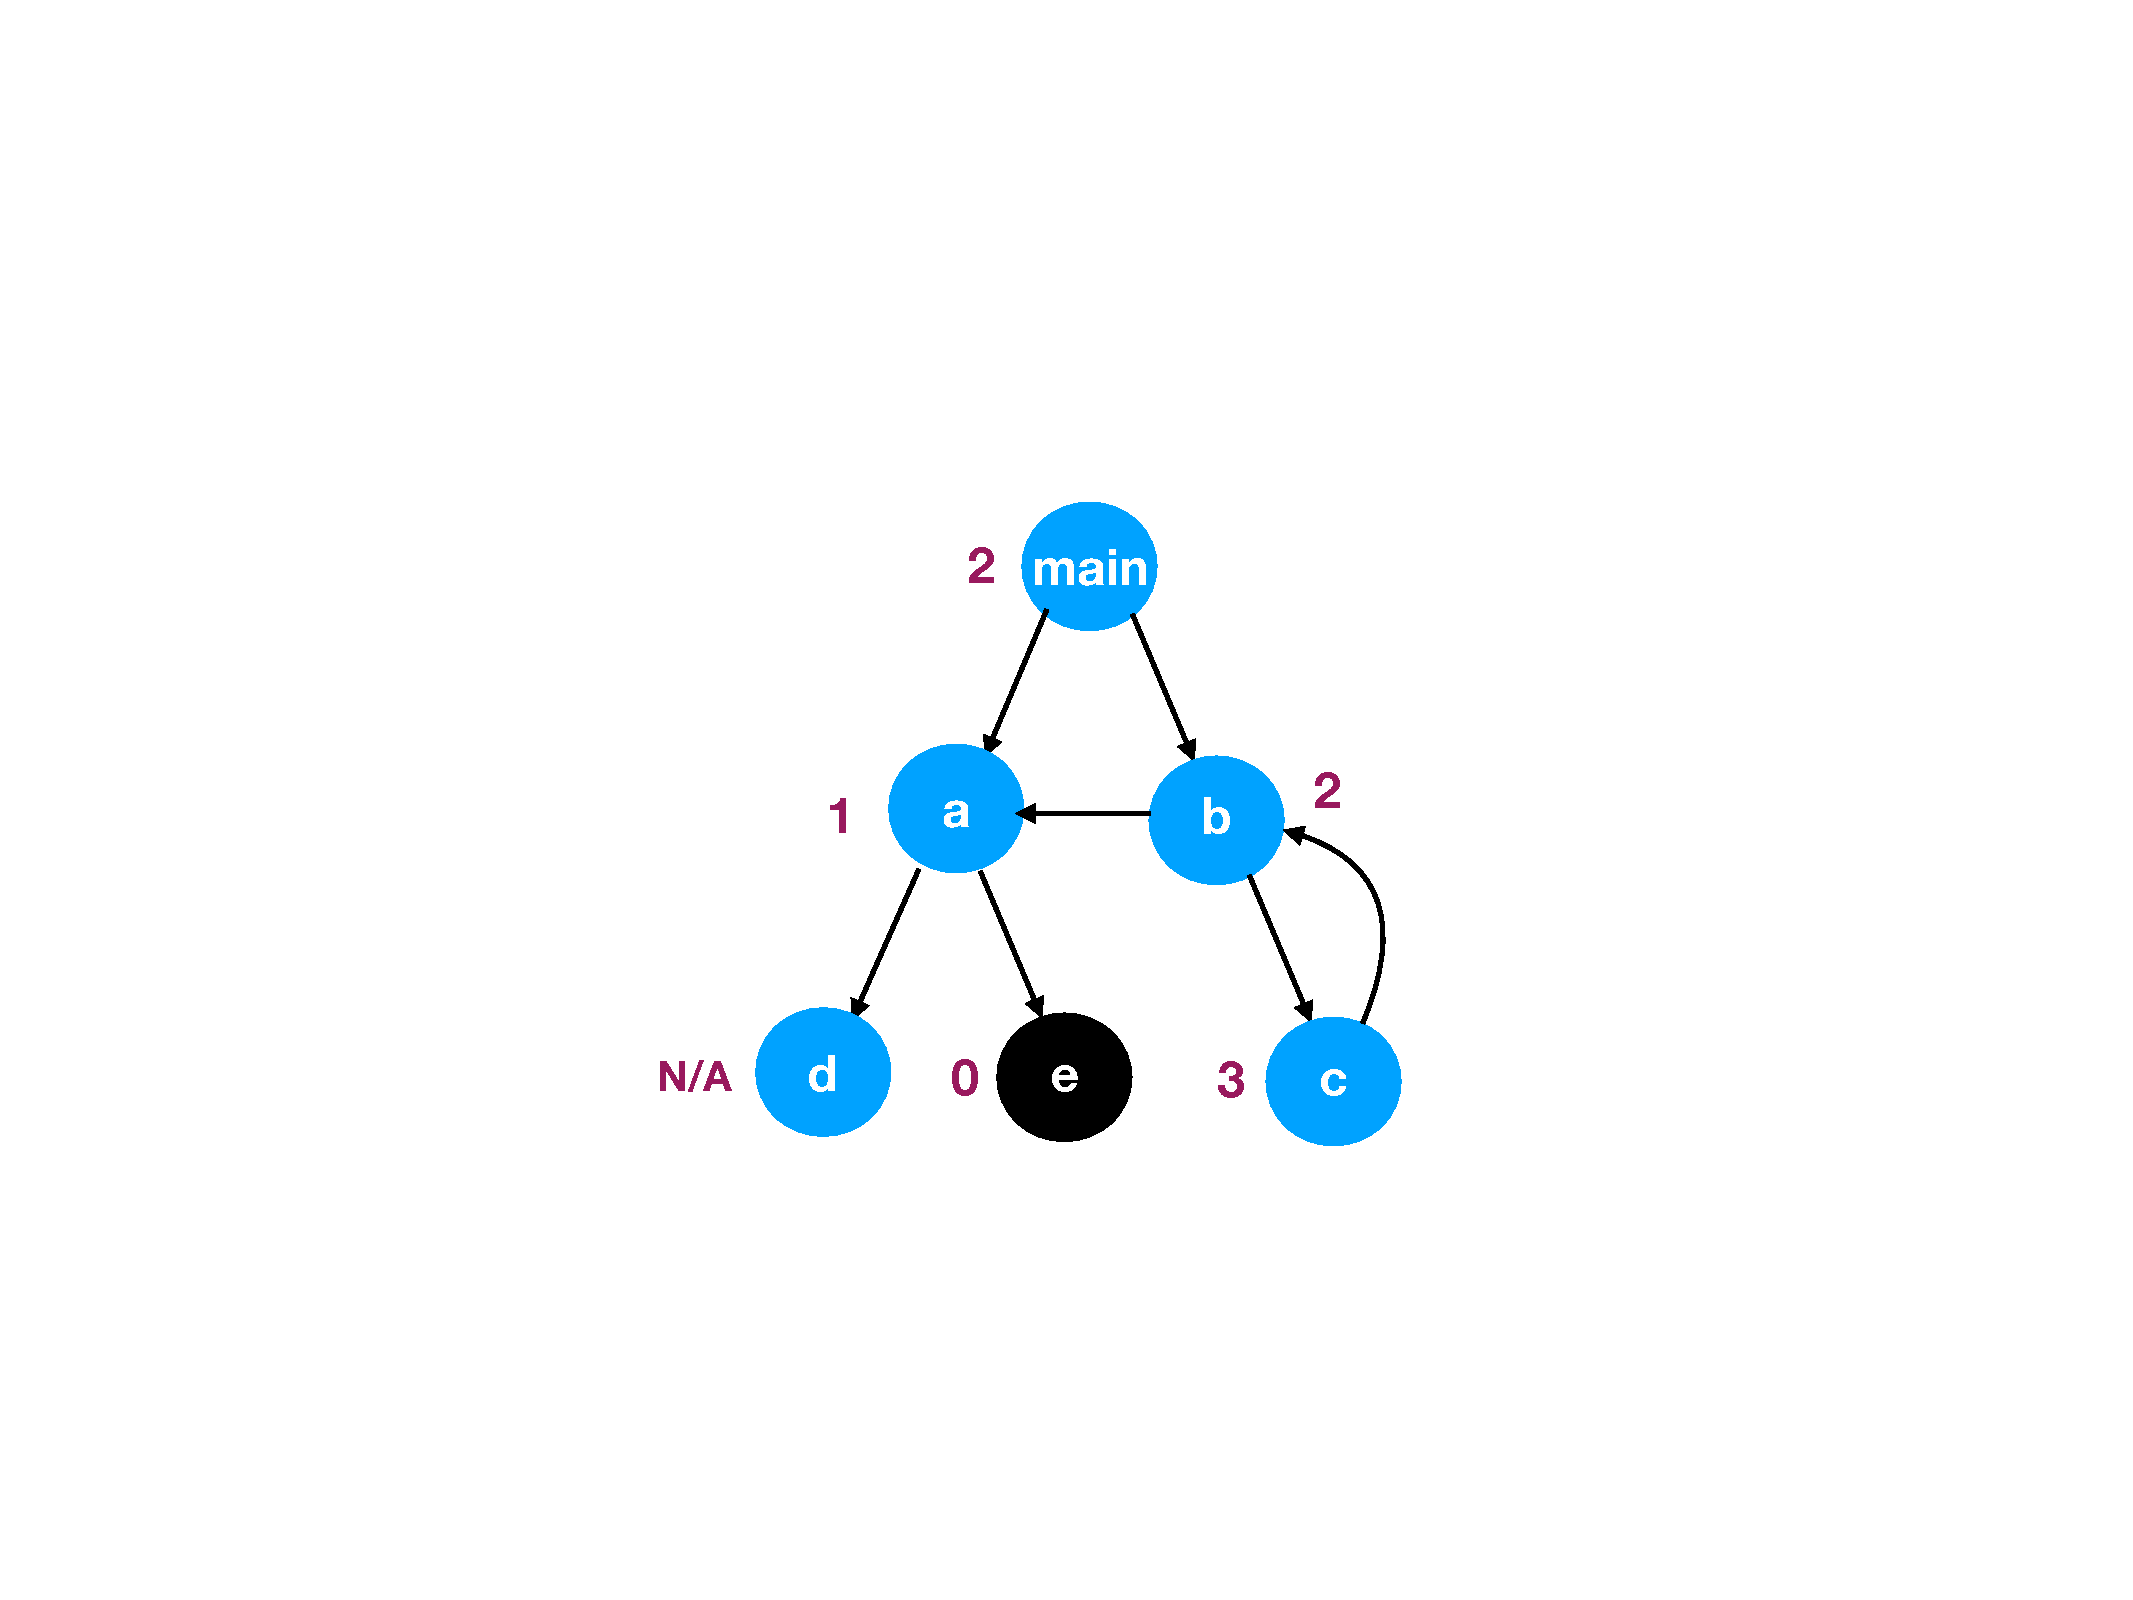
\includegraphics[width=3.5cm]{pic/CG_3.pdf} } 
        \end{minipage}
      \onslide<2->
      \begin{minipage}[t]{0.28\linewidth}
            \vspace{0pt}
            \centering 
            \only<2>{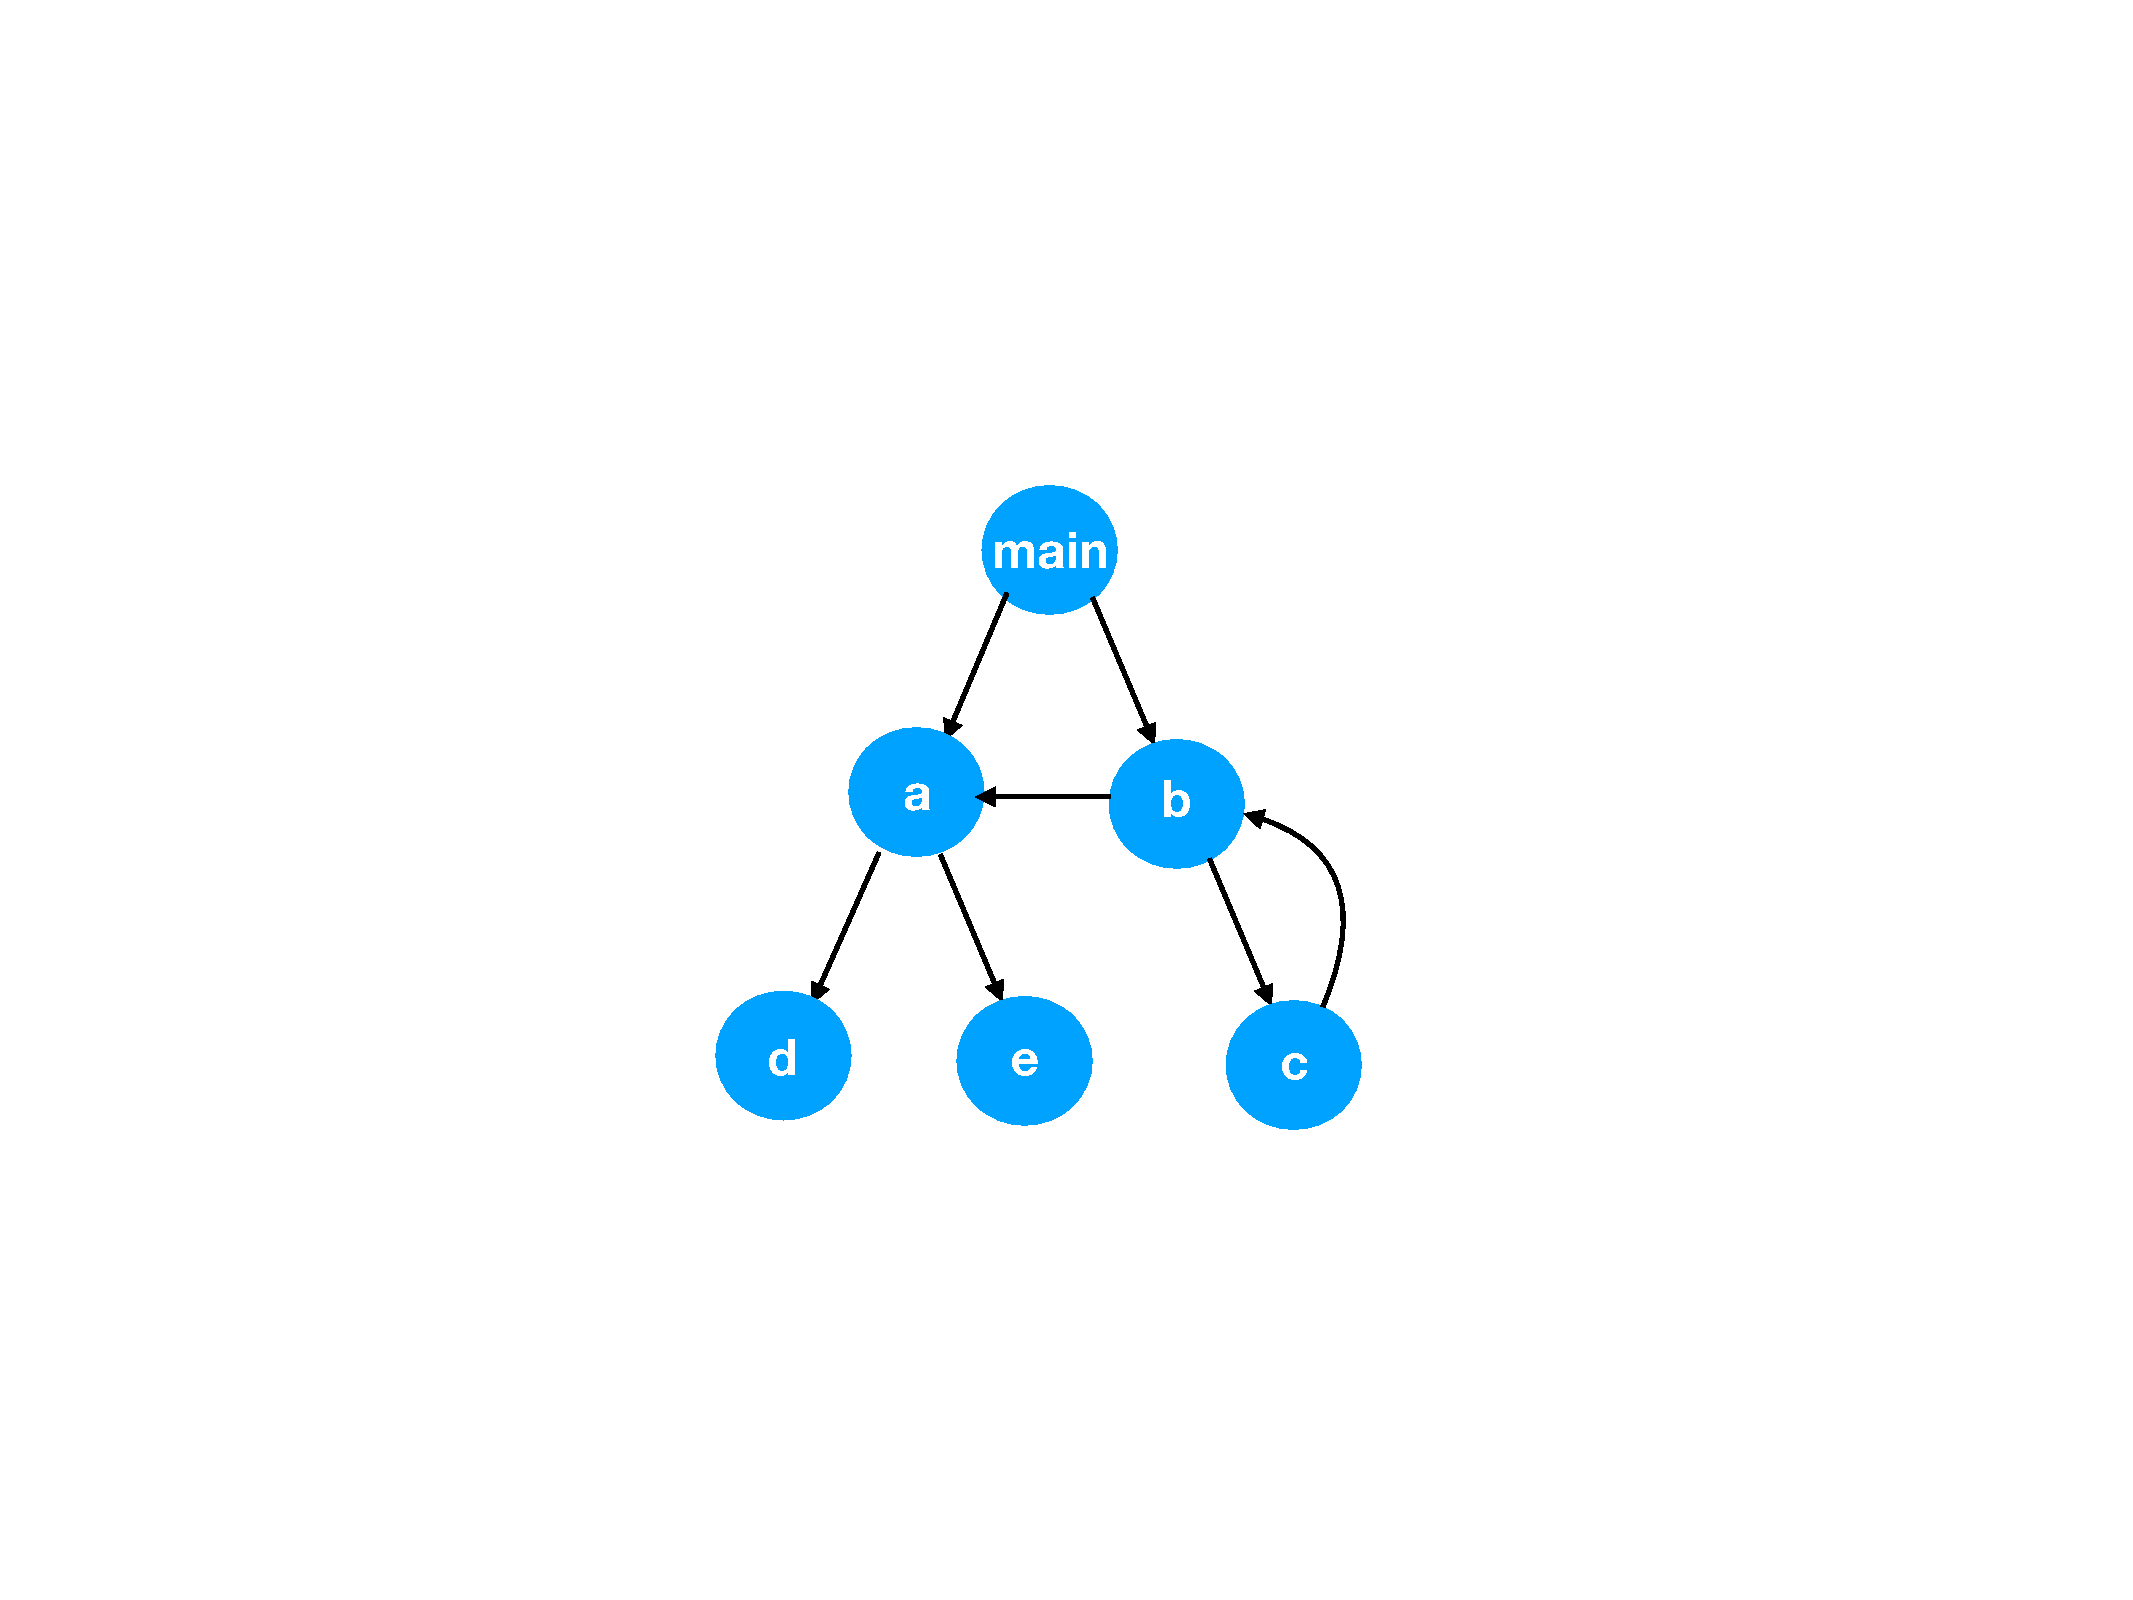
\includegraphics[width=3.0cm]{pic/CG_1.pdf} }
            \only<3>{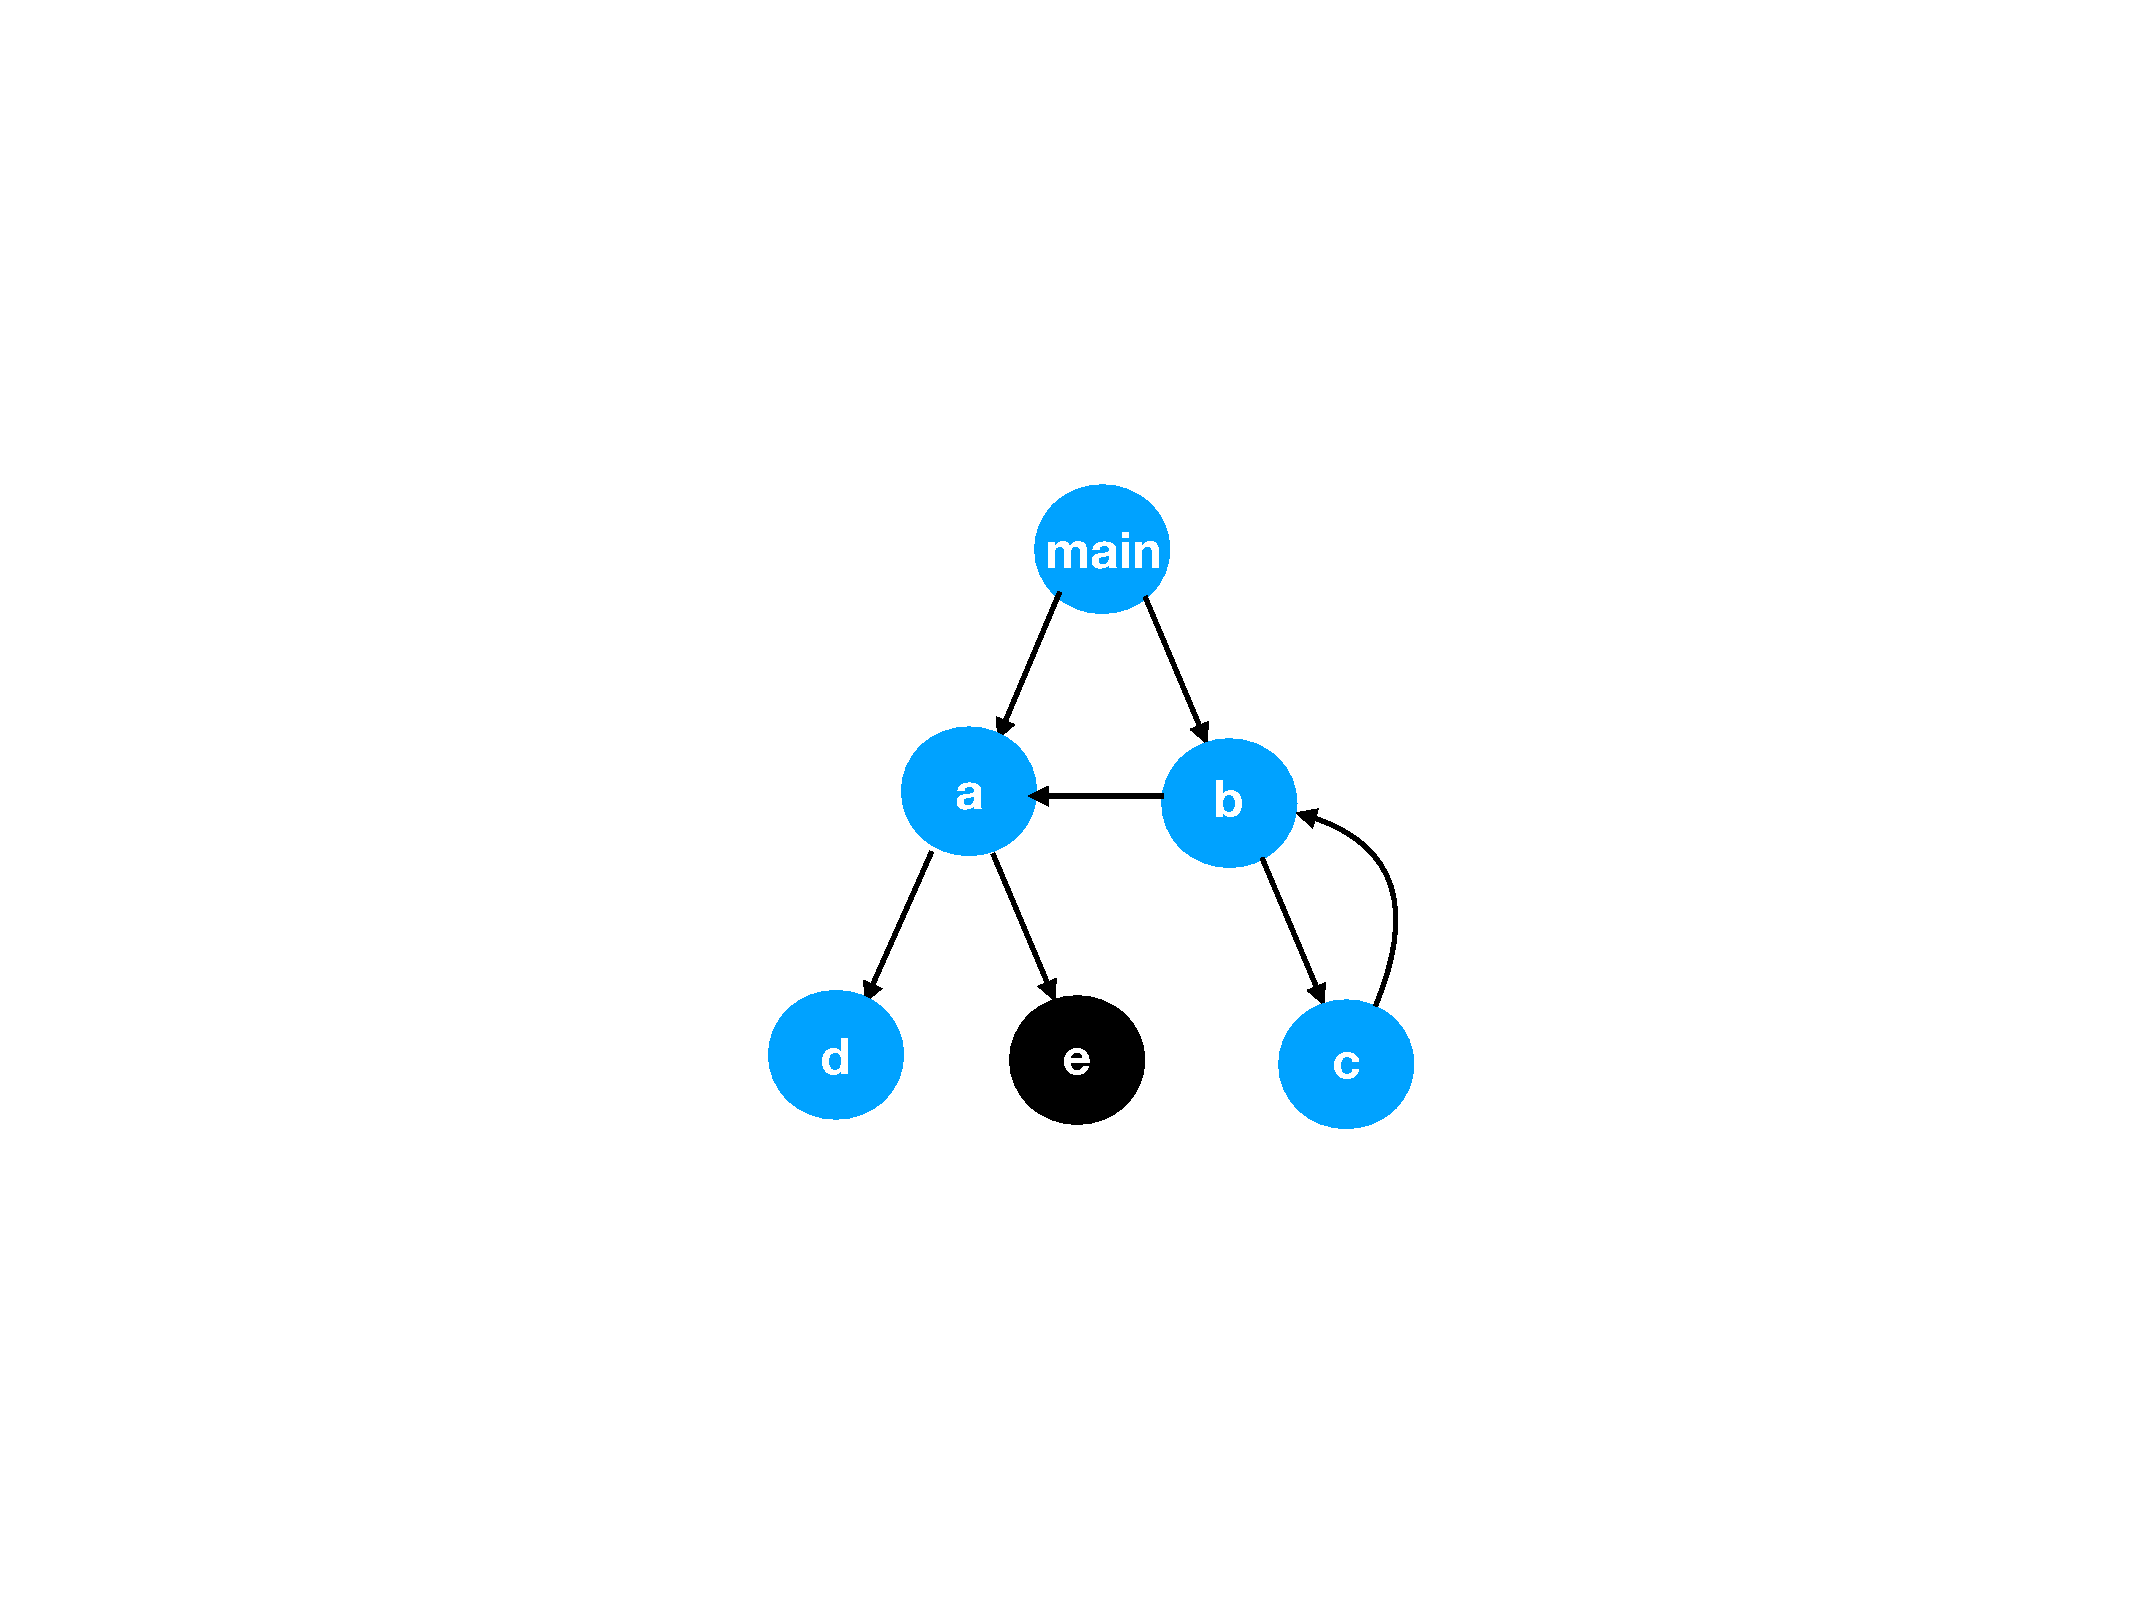
\includegraphics[width=3.0cm]{pic/CG_2.pdf} }
            \only<4>{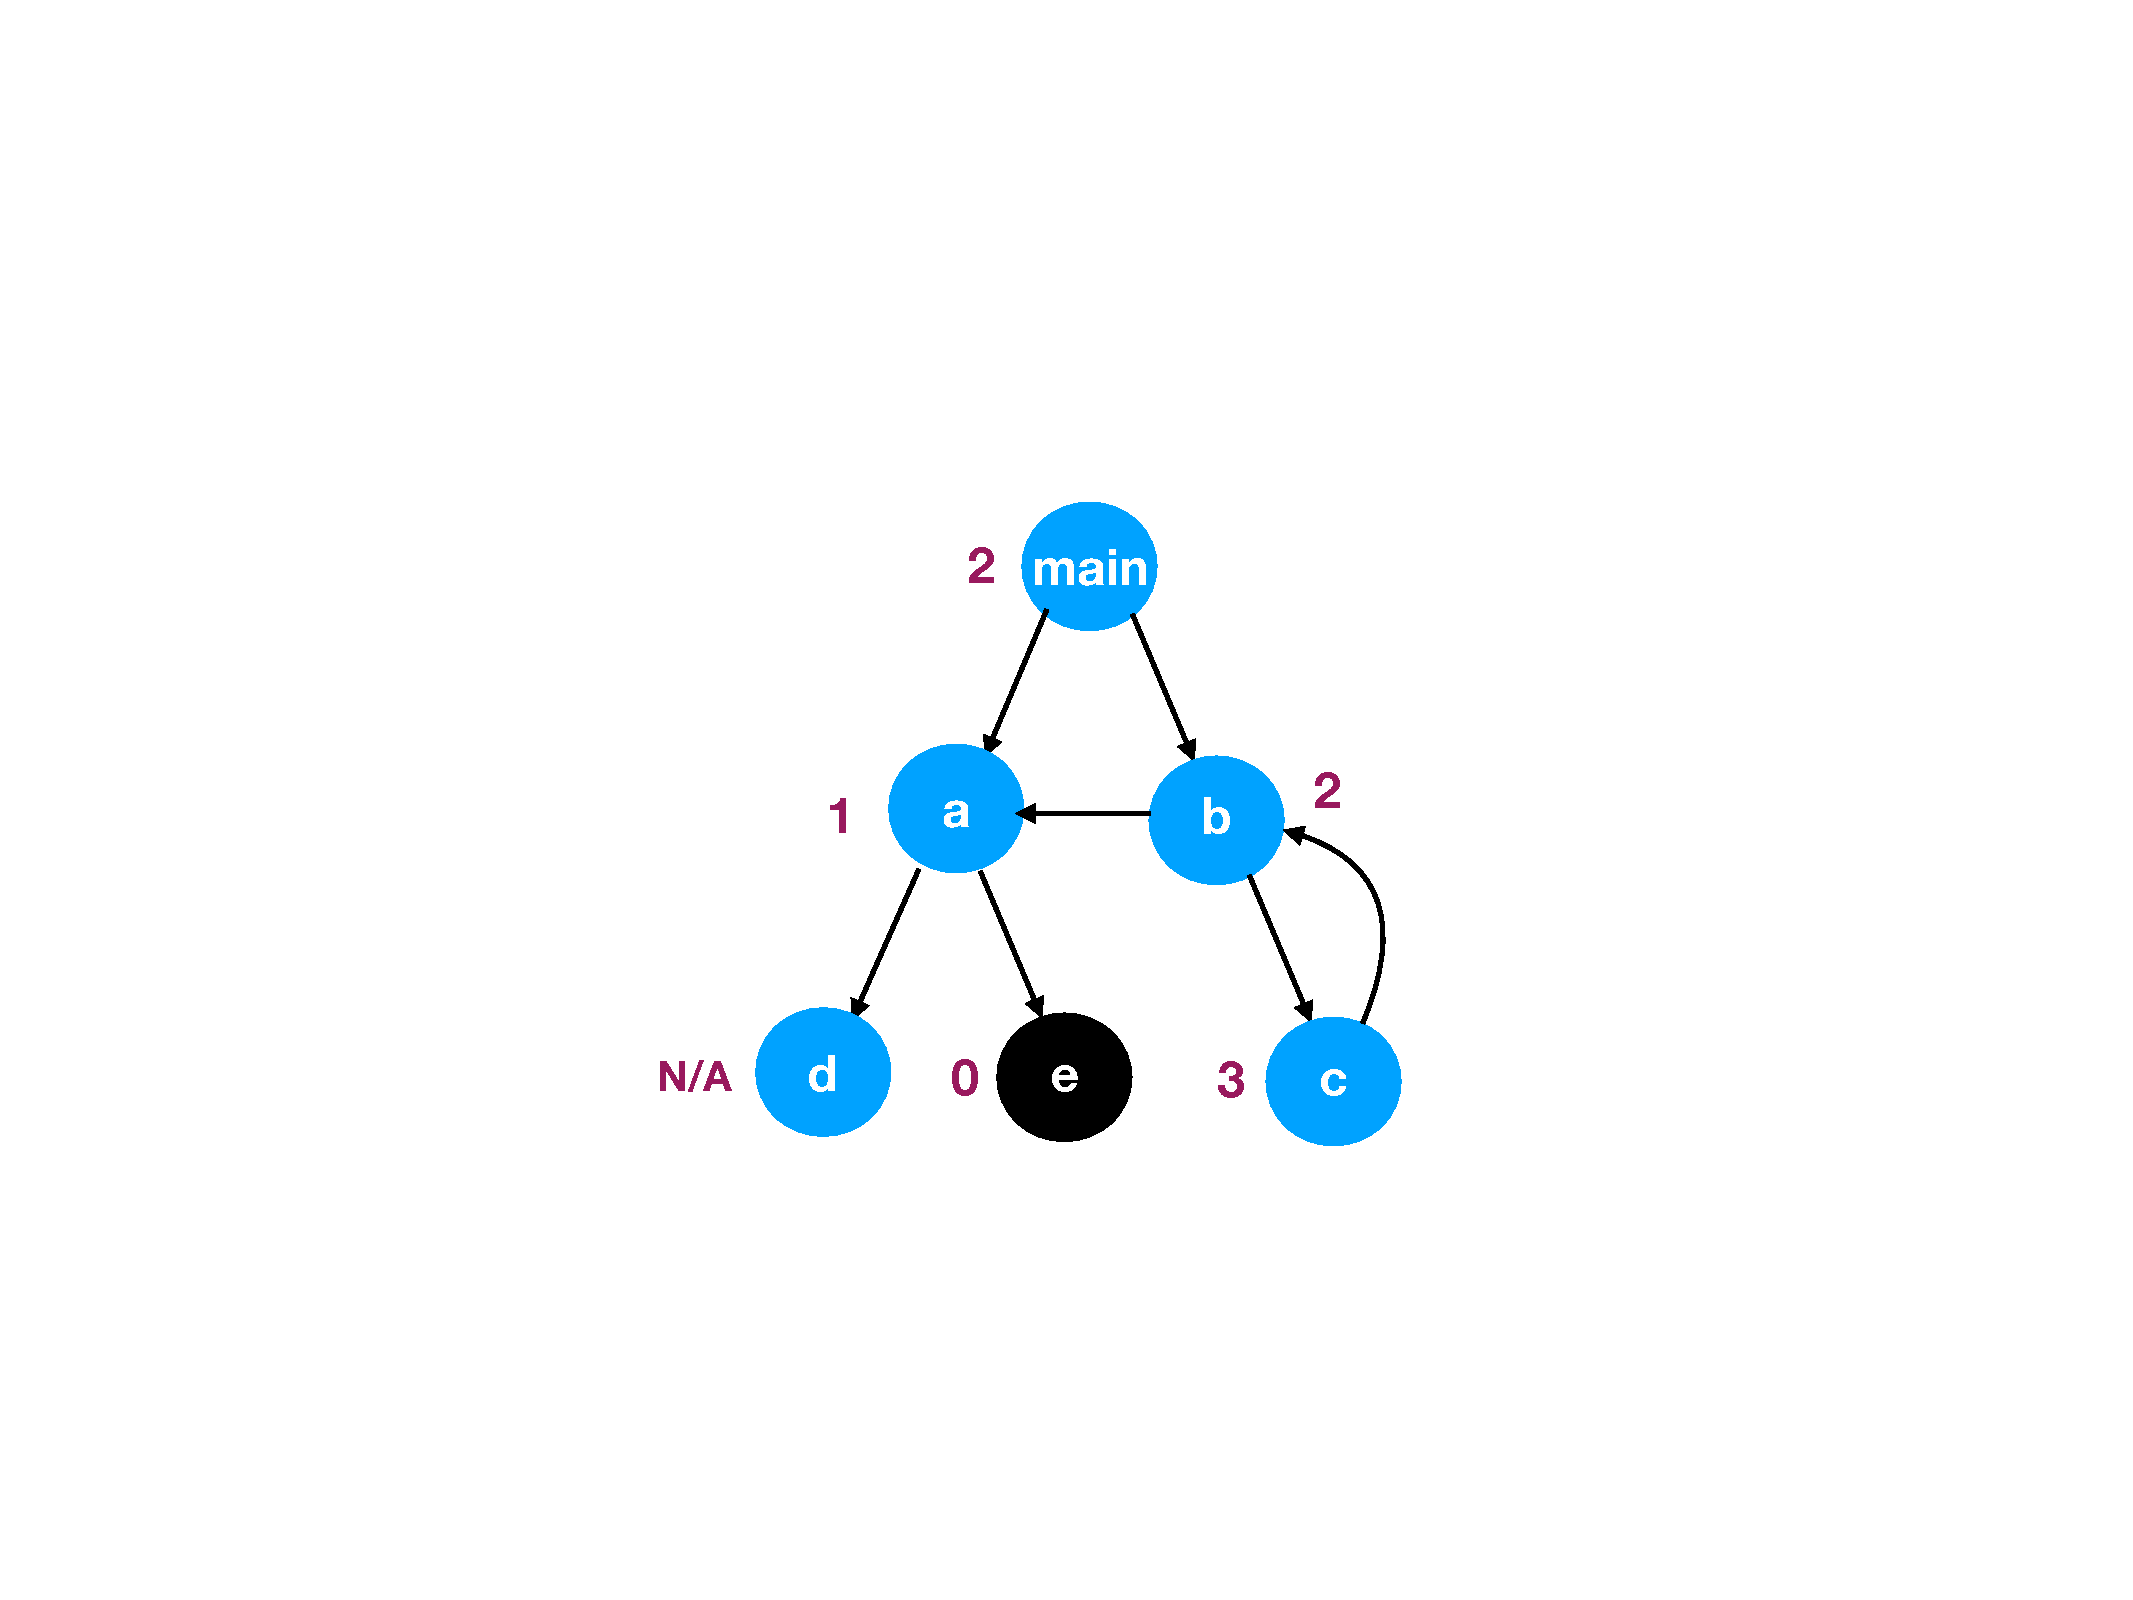
\includegraphics[width=3.5cm]{pic/CG_3.pdf} }
            \only<5-6>{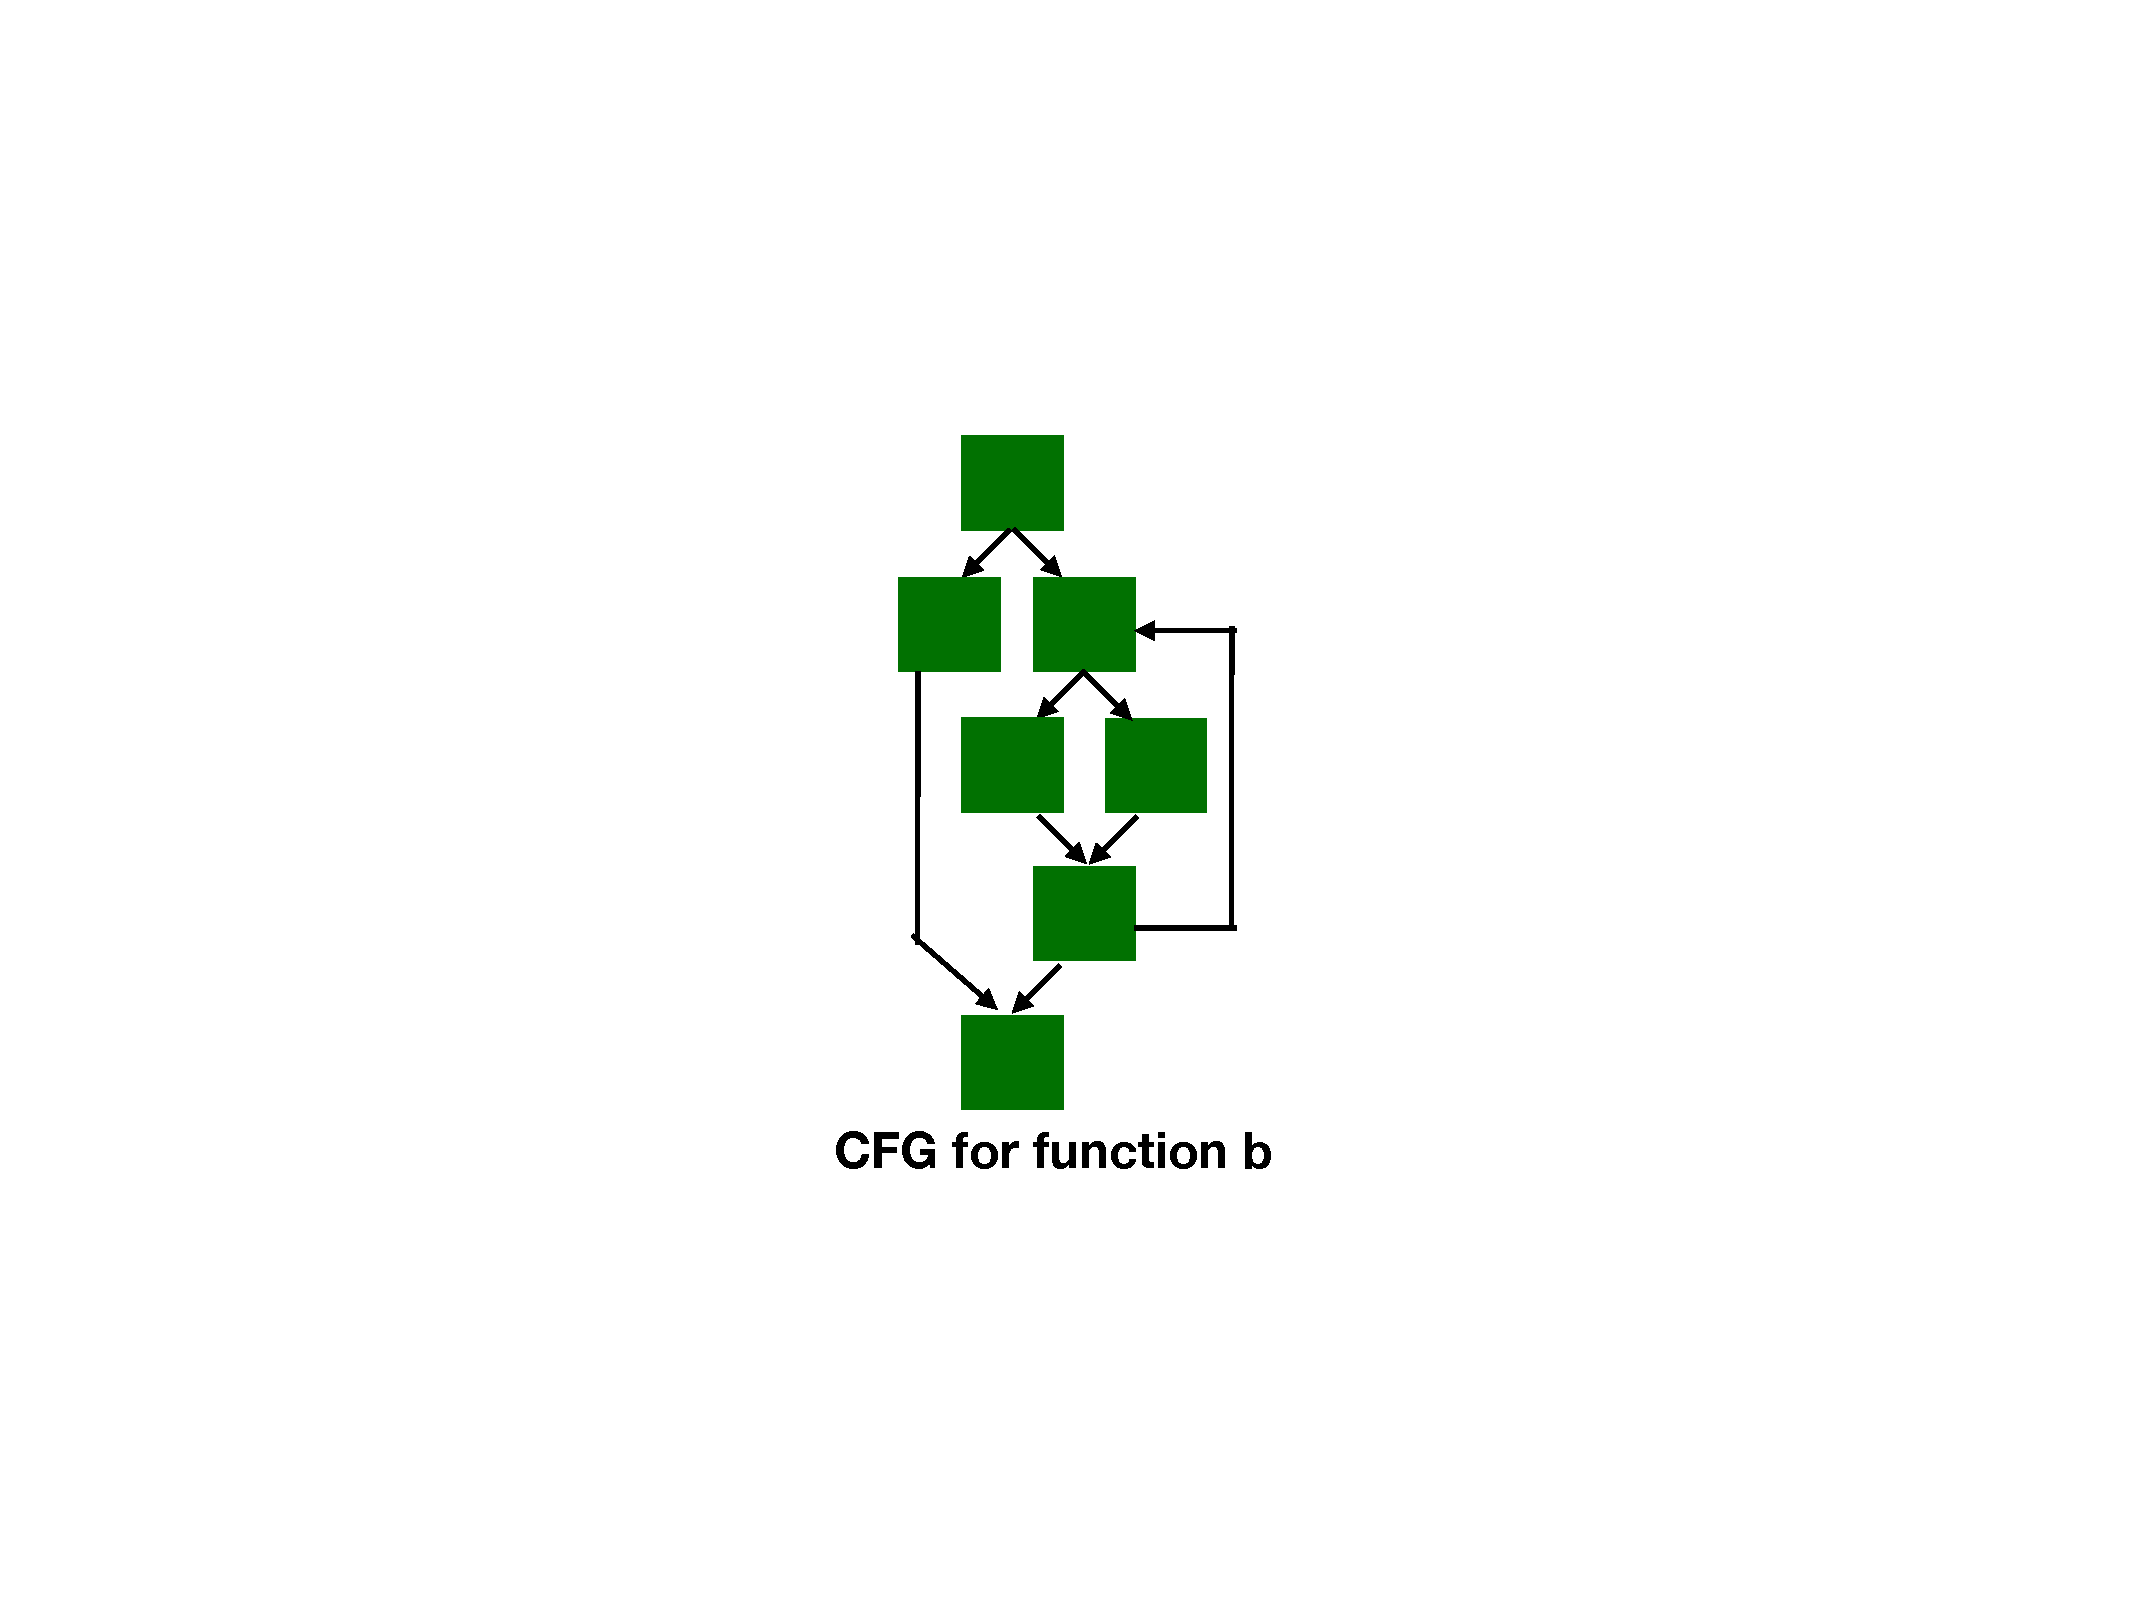
\includegraphics[width=3.5cm]{pic/CFG_1.pdf}}
            \only<7>{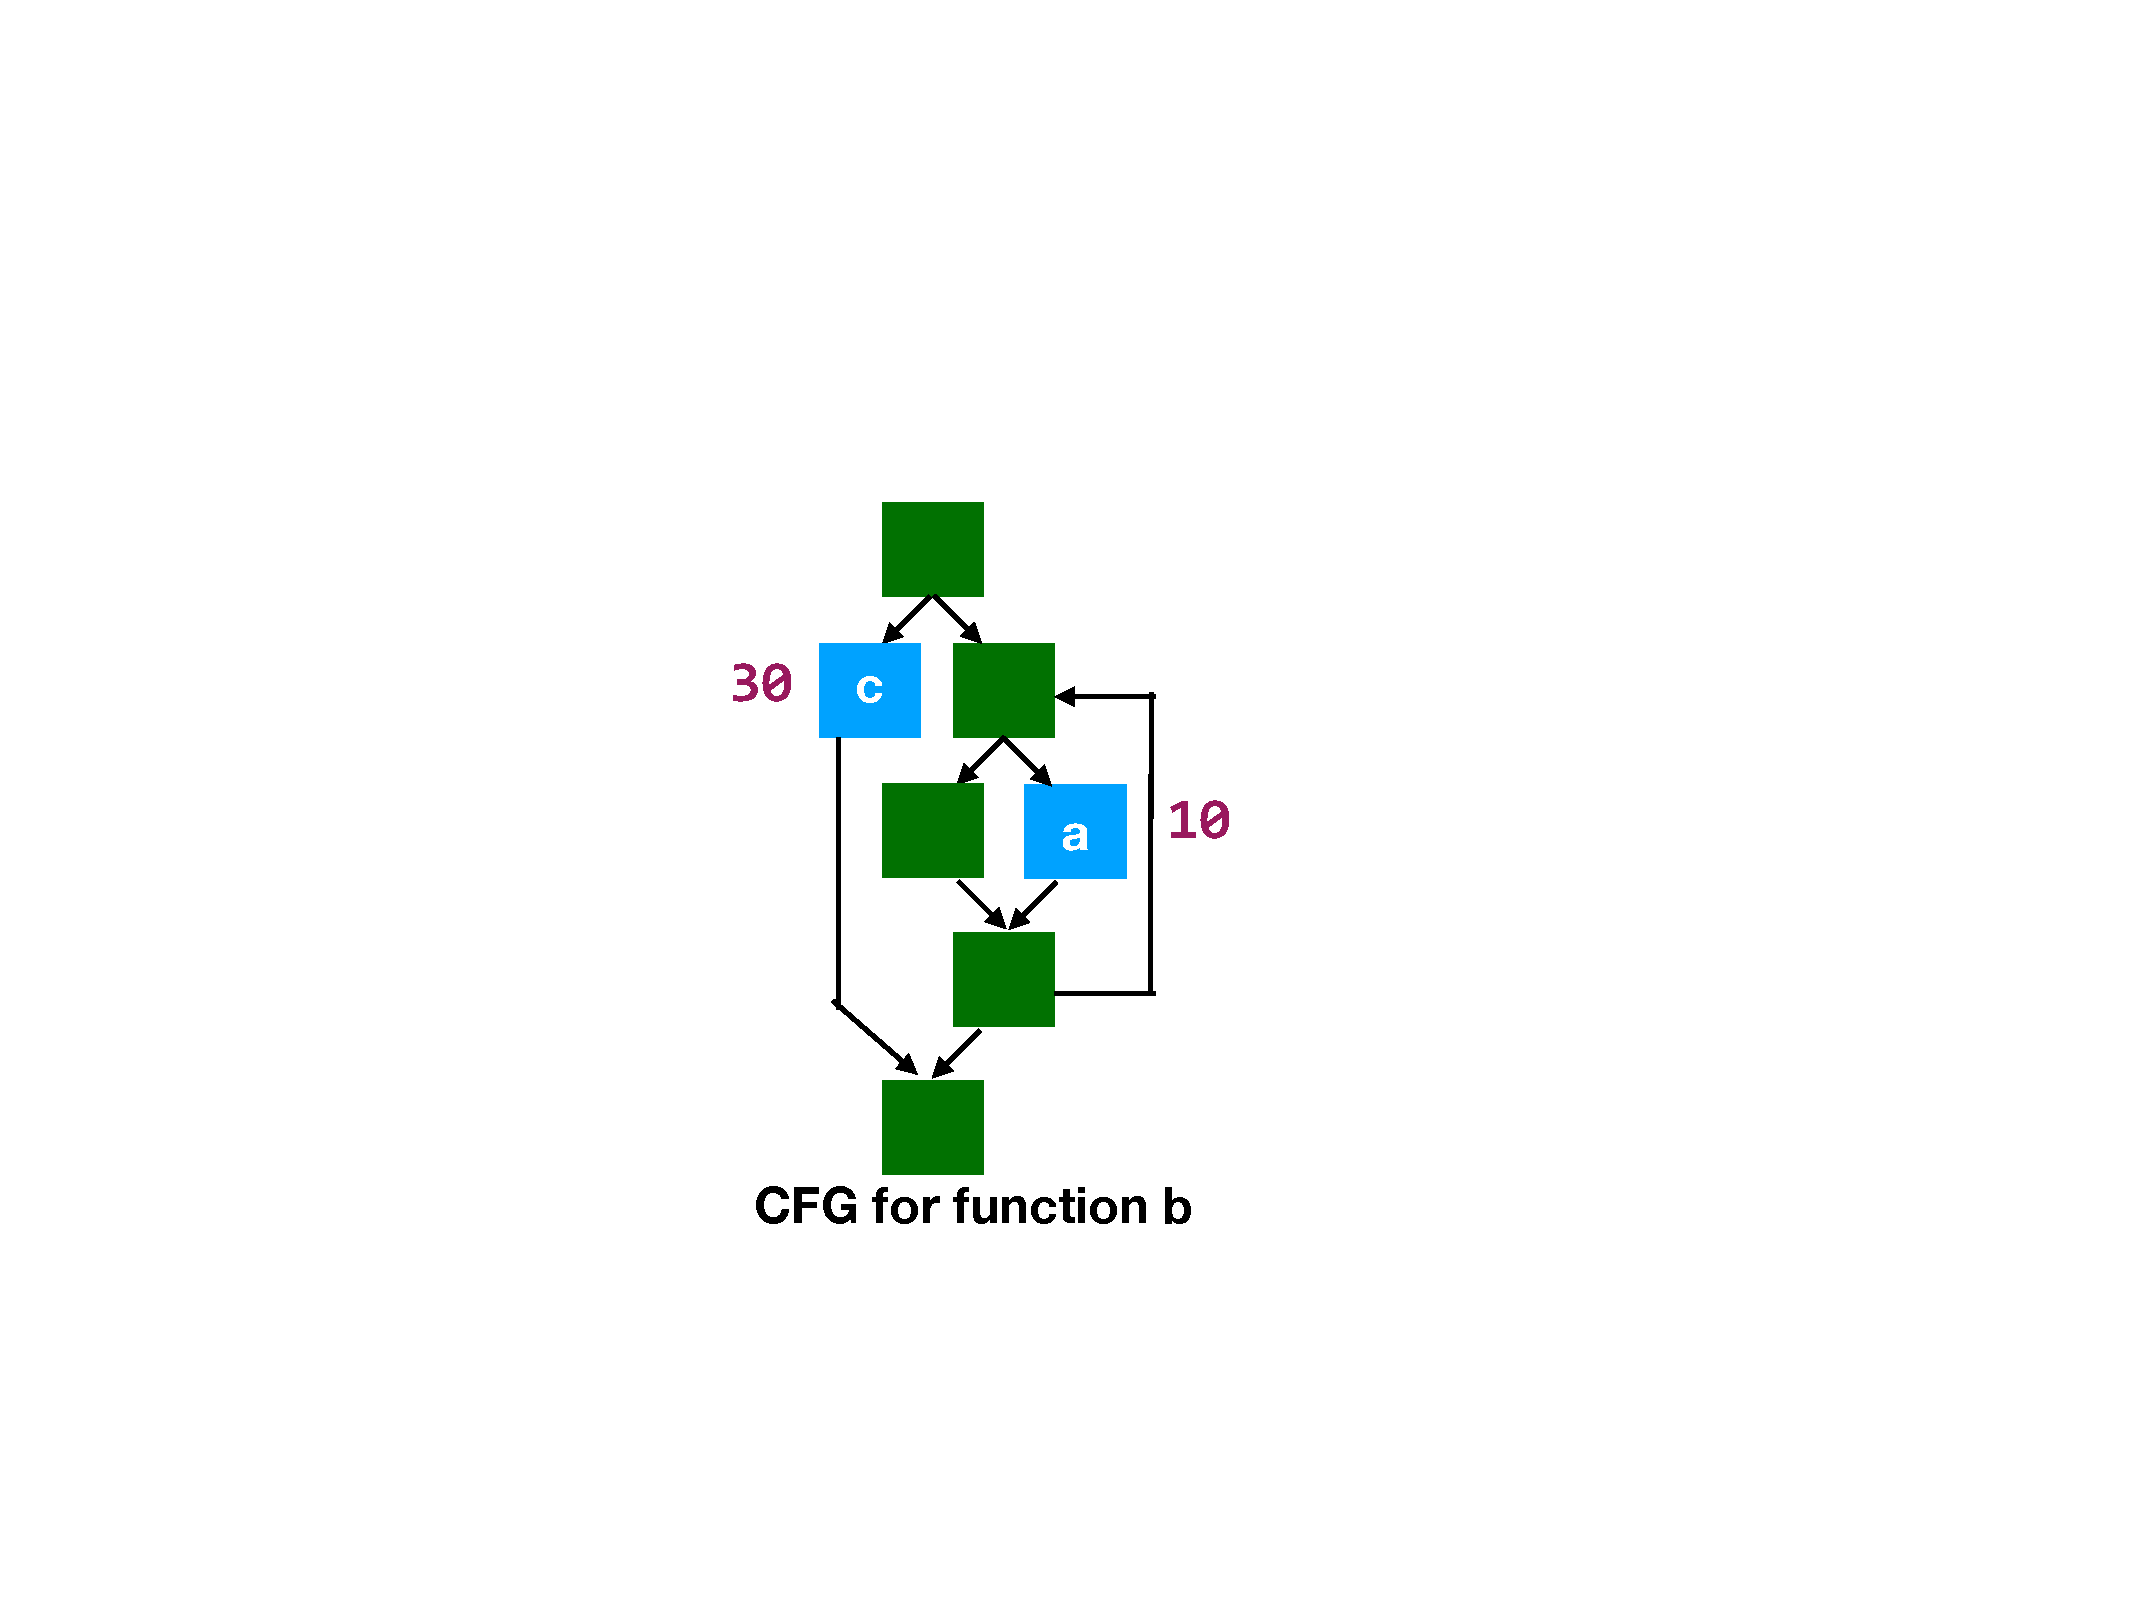
\includegraphics[width=3.5cm]{pic/CFG_2.pdf}}
            \only<8>{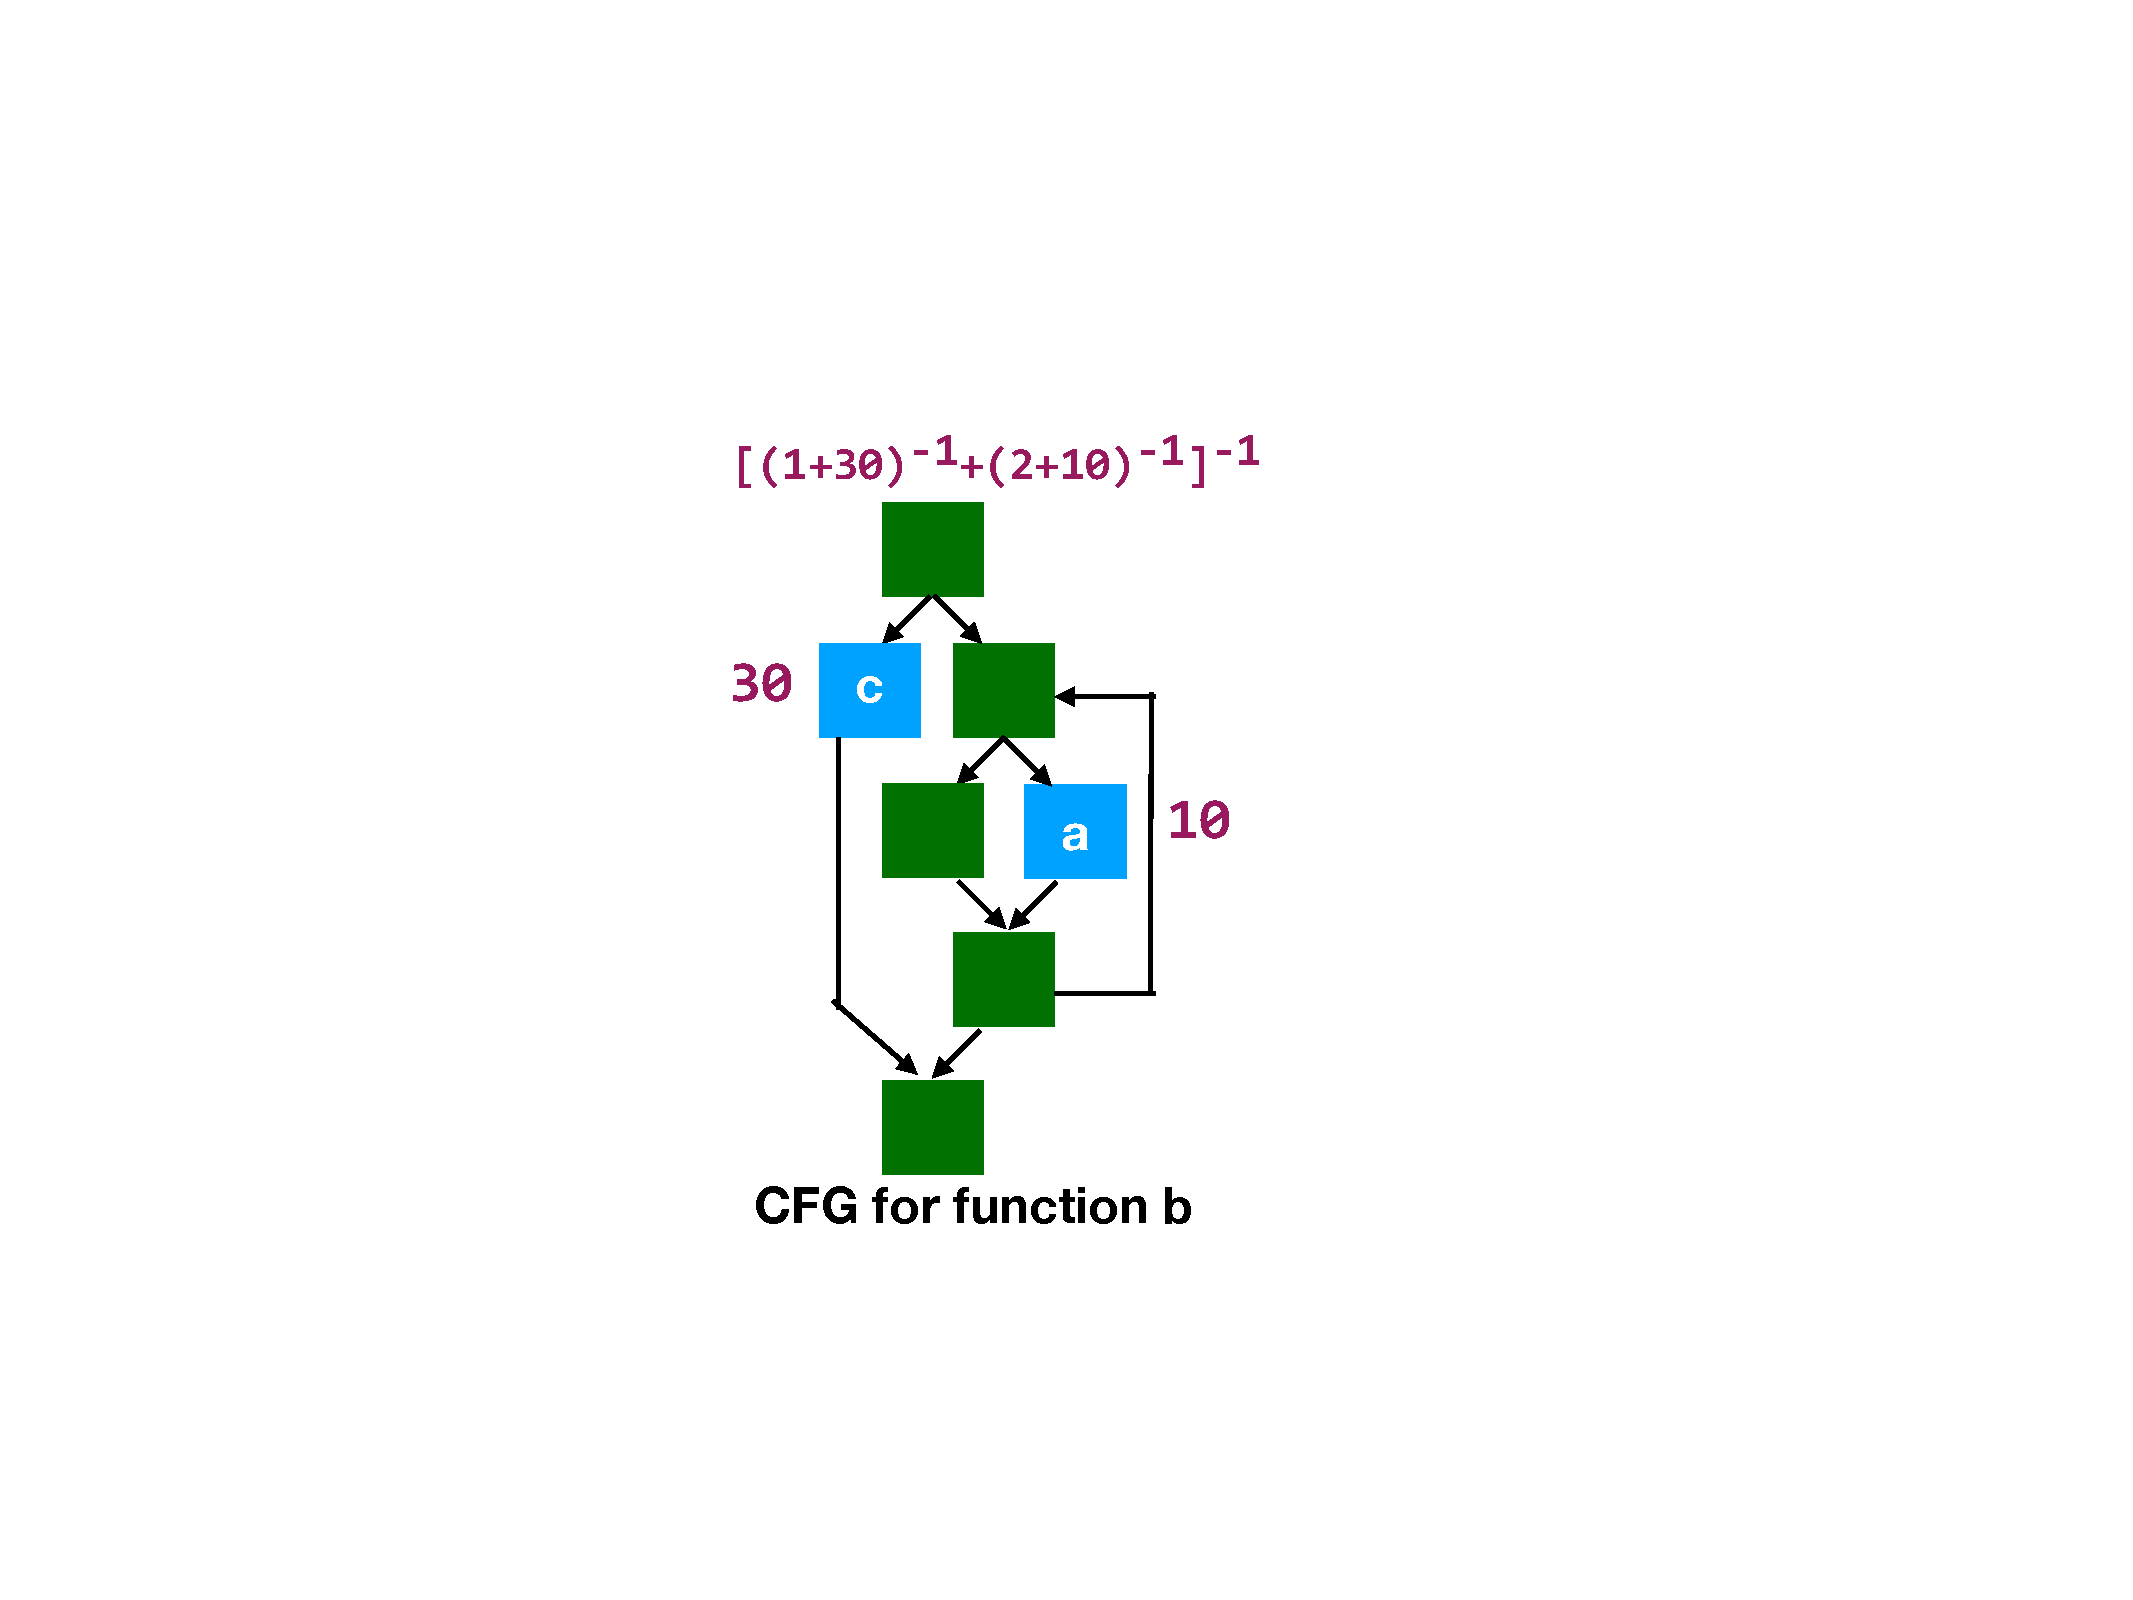
\includegraphics[width=3.5cm]{pic/CFG_3.pdf}}  
            \only<9>{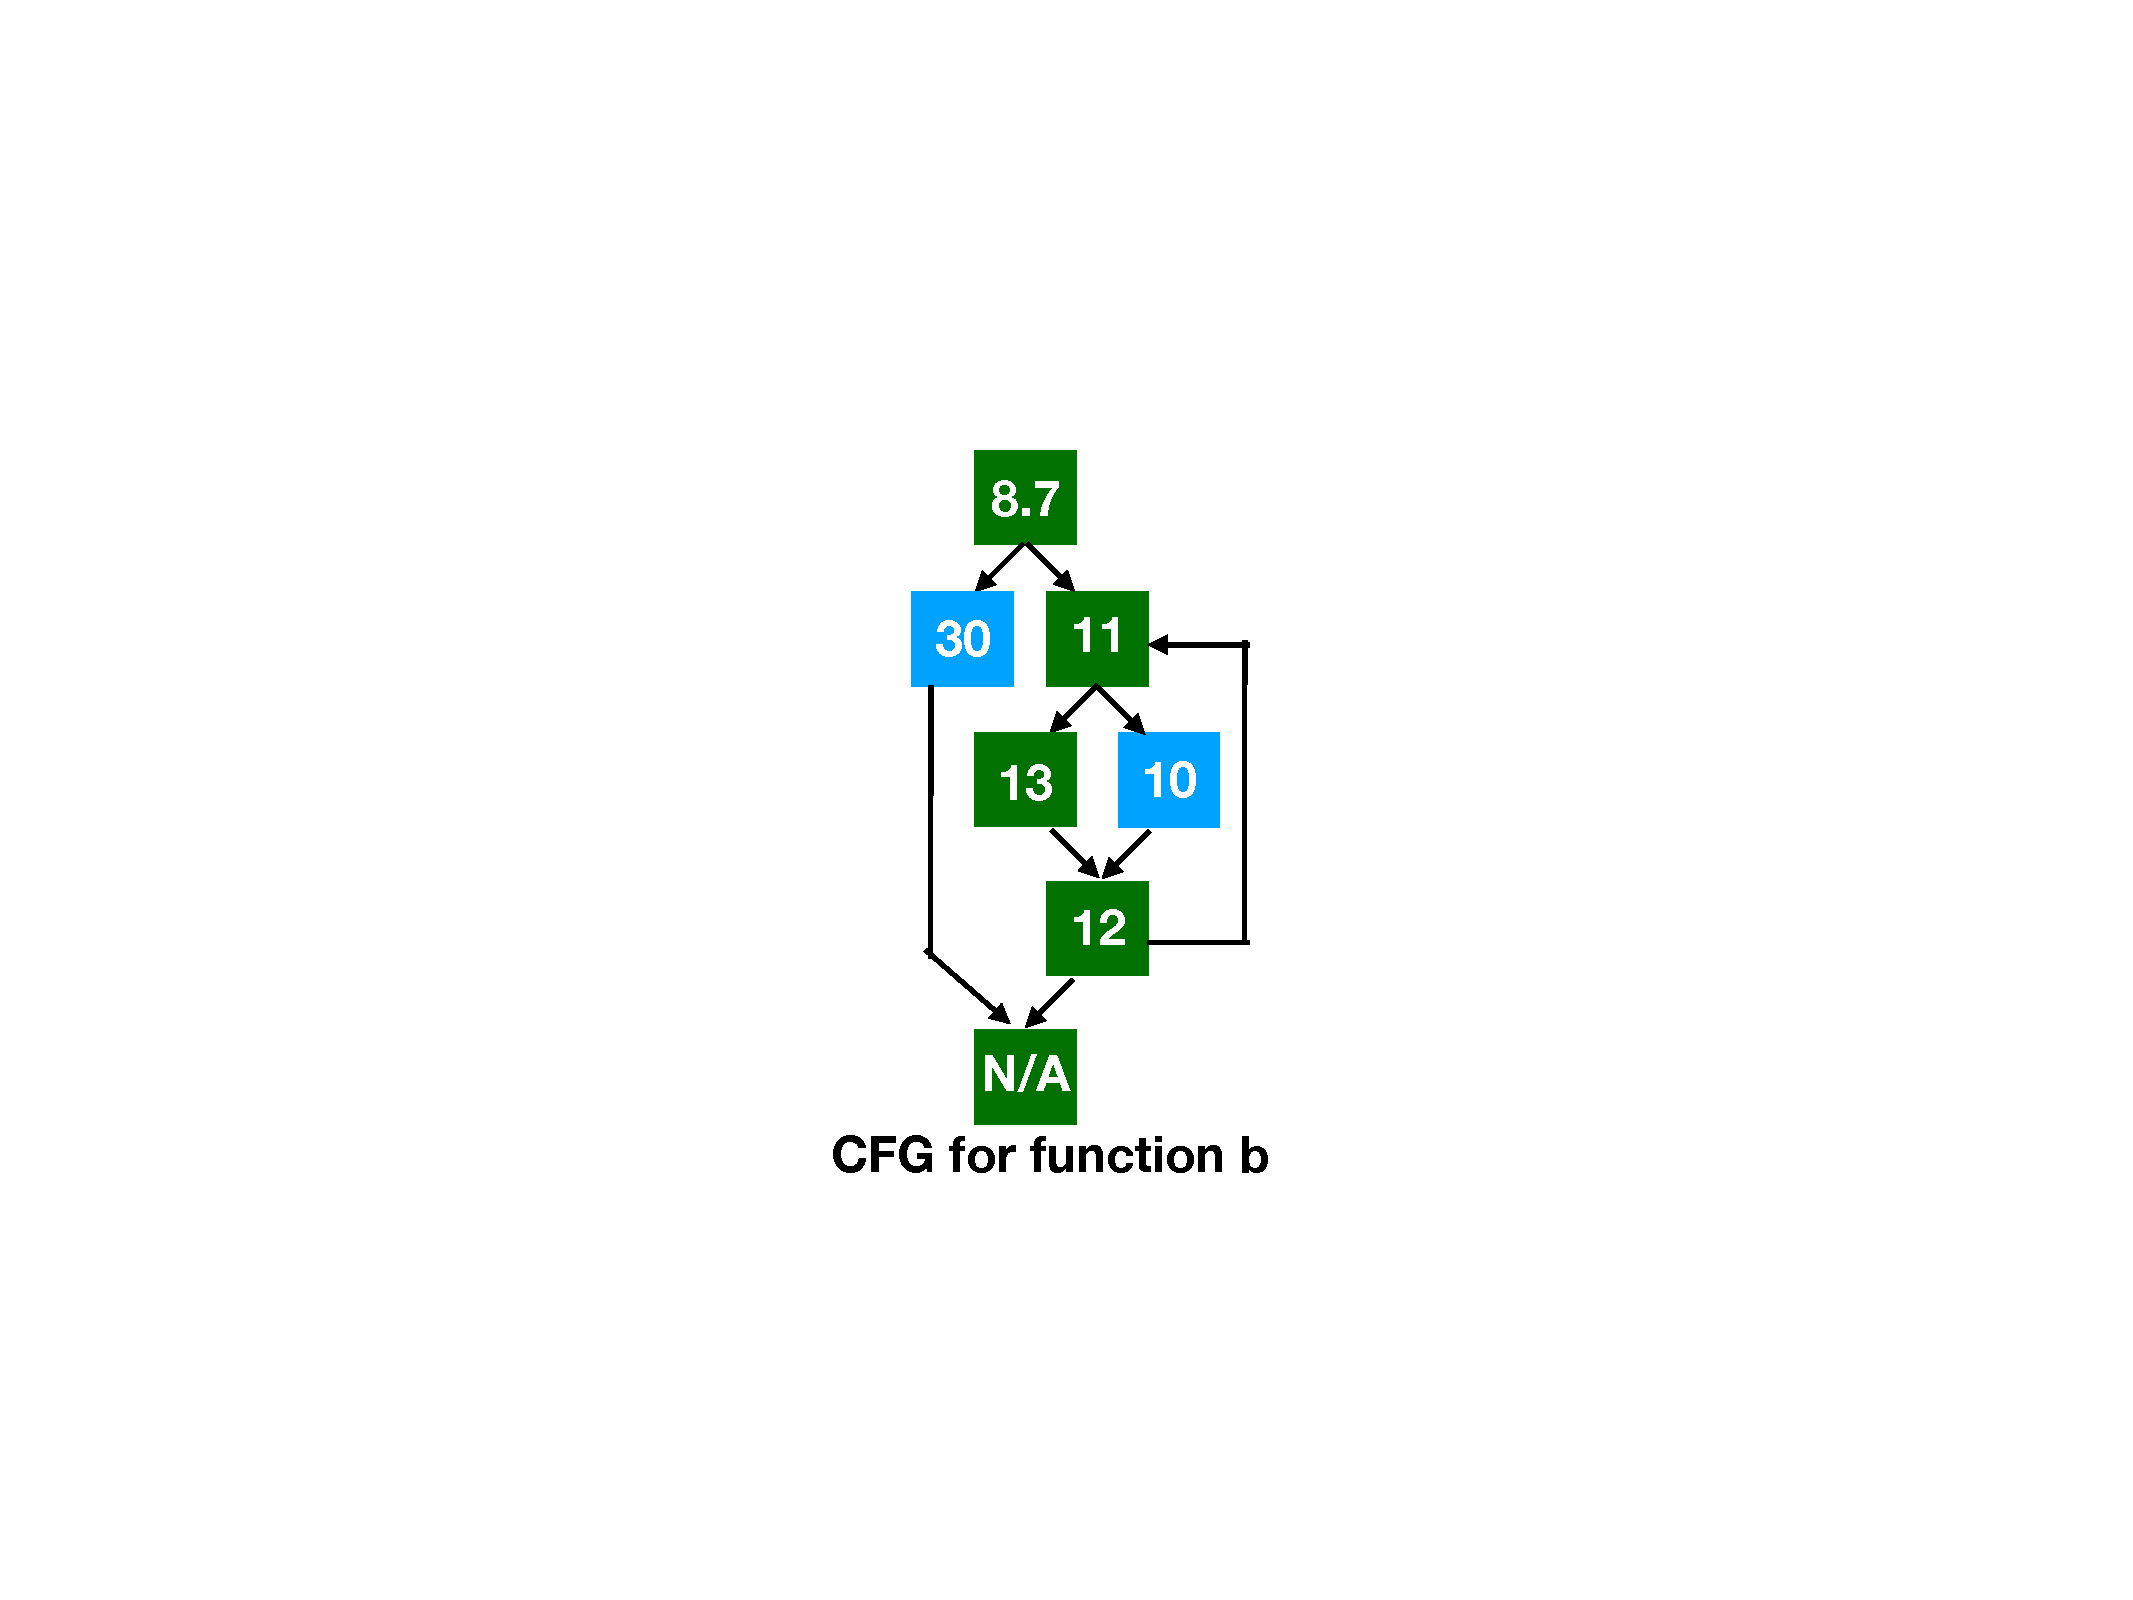
\includegraphics[width=3.5cm]{pic/CFG_4.pdf}}   
       \end{minipage} 
    }
\end{frame}

\begin{frame}{Runtime}
    \only<1>{
        \begin{algorithm}[H]
            \footnotesize
            \DontPrintSemicolon
            \SetKwSty{algokeywordsty}
            \SetFuncSty{algofuncsty}
            \SetDataSty{algodatasty}
            \SetArgSty{algoargsty}
            \SetCommentSty{algocmtsty}
            \SetKw{break}{break}
            \SetKw{not}{not}
            \SetKwFunction{graphextractor}{\textsc{GraphExt}}
            \SetKwFunction{bbdistance}{\textsc{DisCalcu}}  
            \SetKwFunction{select}{\textsc{Dequeue}}
            \SetKwFunction{assinenergy}{\textsc{AssinEnergy}}
            \SetKwFunction{mutation}{\textsc{Mutation}}
            \SetKwFunction{execution}{\textsc{Execution}}
            \SetKwFunction{IsIntersting}{\textsc{IsIntersting}}
            \SetKwFunction{evaluateseed}{\textsc{SeedDis}}
            \SetKwFunction{sortinsert}{Enqueue}
            % \SetKwData{crashseeds}{$\seeds_{\text{\emoji{boom}}}$}
            \SetKwData{crashseeds}{$\seeds^\prime$} 
            \SetKwData{seedqueue}{$\textit{SeedQueue}$}  
            \SetKwData{Graph}{$\textit{Graphs}$}  
            \SetKwData{BBdis}{$\textit{BBdistance}$} 
            \SetKwData{newseed}{$\seed^\prime$}   
            \SetKwData{energy}{$\textit{e}$}
            \SetKwData{trace}{$\textit{trace}$} 
            \SetKwData{distance}{$\textit{distance}$}   
            \KwIn{\seeds\tcp{a finite set of seeds}}
            \KwIn{\targets\tcp{a finite set of targer sits}} 
            \KwOut{\crashseeds \tcp{a finite set of buggy seeds}}
            $\crashseeds\gets \varnothing$\; 
            $\seedqueue \gets \seeds$\;
            \Graph $\gets \graphextractor{\sourcecode}$\;
            \BBdis $\gets \bbdistance{\targets,\Graph}$\;
            \While {$!siganl \land \currtime < \timeout$}{
              \seed$\gets \select{\seedqueue}$\;
              $\trace \gets \execution{\seed}$\; 
              \HiLi$\distance \gets \evaluateseed{\trace, \BBdis} $\;
              \HiLi\energy $\gets \assinenergy{\seed, \currtime, \distance}$\;
               \For{$\textit{i}\gets 1$ \KwTo $\energy$}
               {
                $\newseed \gets \mutation{\seed}$\;      
                \lIf{\newseed crashes}{$\crashseeds \gets \crashseeds \cup \newseed $}
                \lIf{\IsIntersting{\newseed}}{    
                    $\sortinsert{\newseed,\seedqueue} $ 
                }
               }
            }
            \Return{\crashseeds}\;
        \end{algorithm} 
    }
    \only<2-4>{
        \begin{minipage}[t]{0.7\linewidth}
        \vspace{0pt} 
        \textbf{\structure {Seed distance\only<2>{\footnote{$\xi(s)$ is the execution trace of a seed s}}}} from instrumented binary
        \only<2>{
            $$ d(s,T_b)=\frac{\sum\limits_{m \in \xi (s)}d_b(m,T_b)}{| \xi(s)| }$$
        }
        \only<3-4>{
            \begin{itemize}
               \item  Two 64-bit shared memory entries
                    \\• Aggregated BB-level distance values
                    \\• Number of executed BBs
            \end{itemize}
        }
        \end{minipage}
      \onslide<2-4>
      \begin{minipage}[t]{0.28\linewidth}
            \vspace{0pt}
            \centering 
            \only<2>{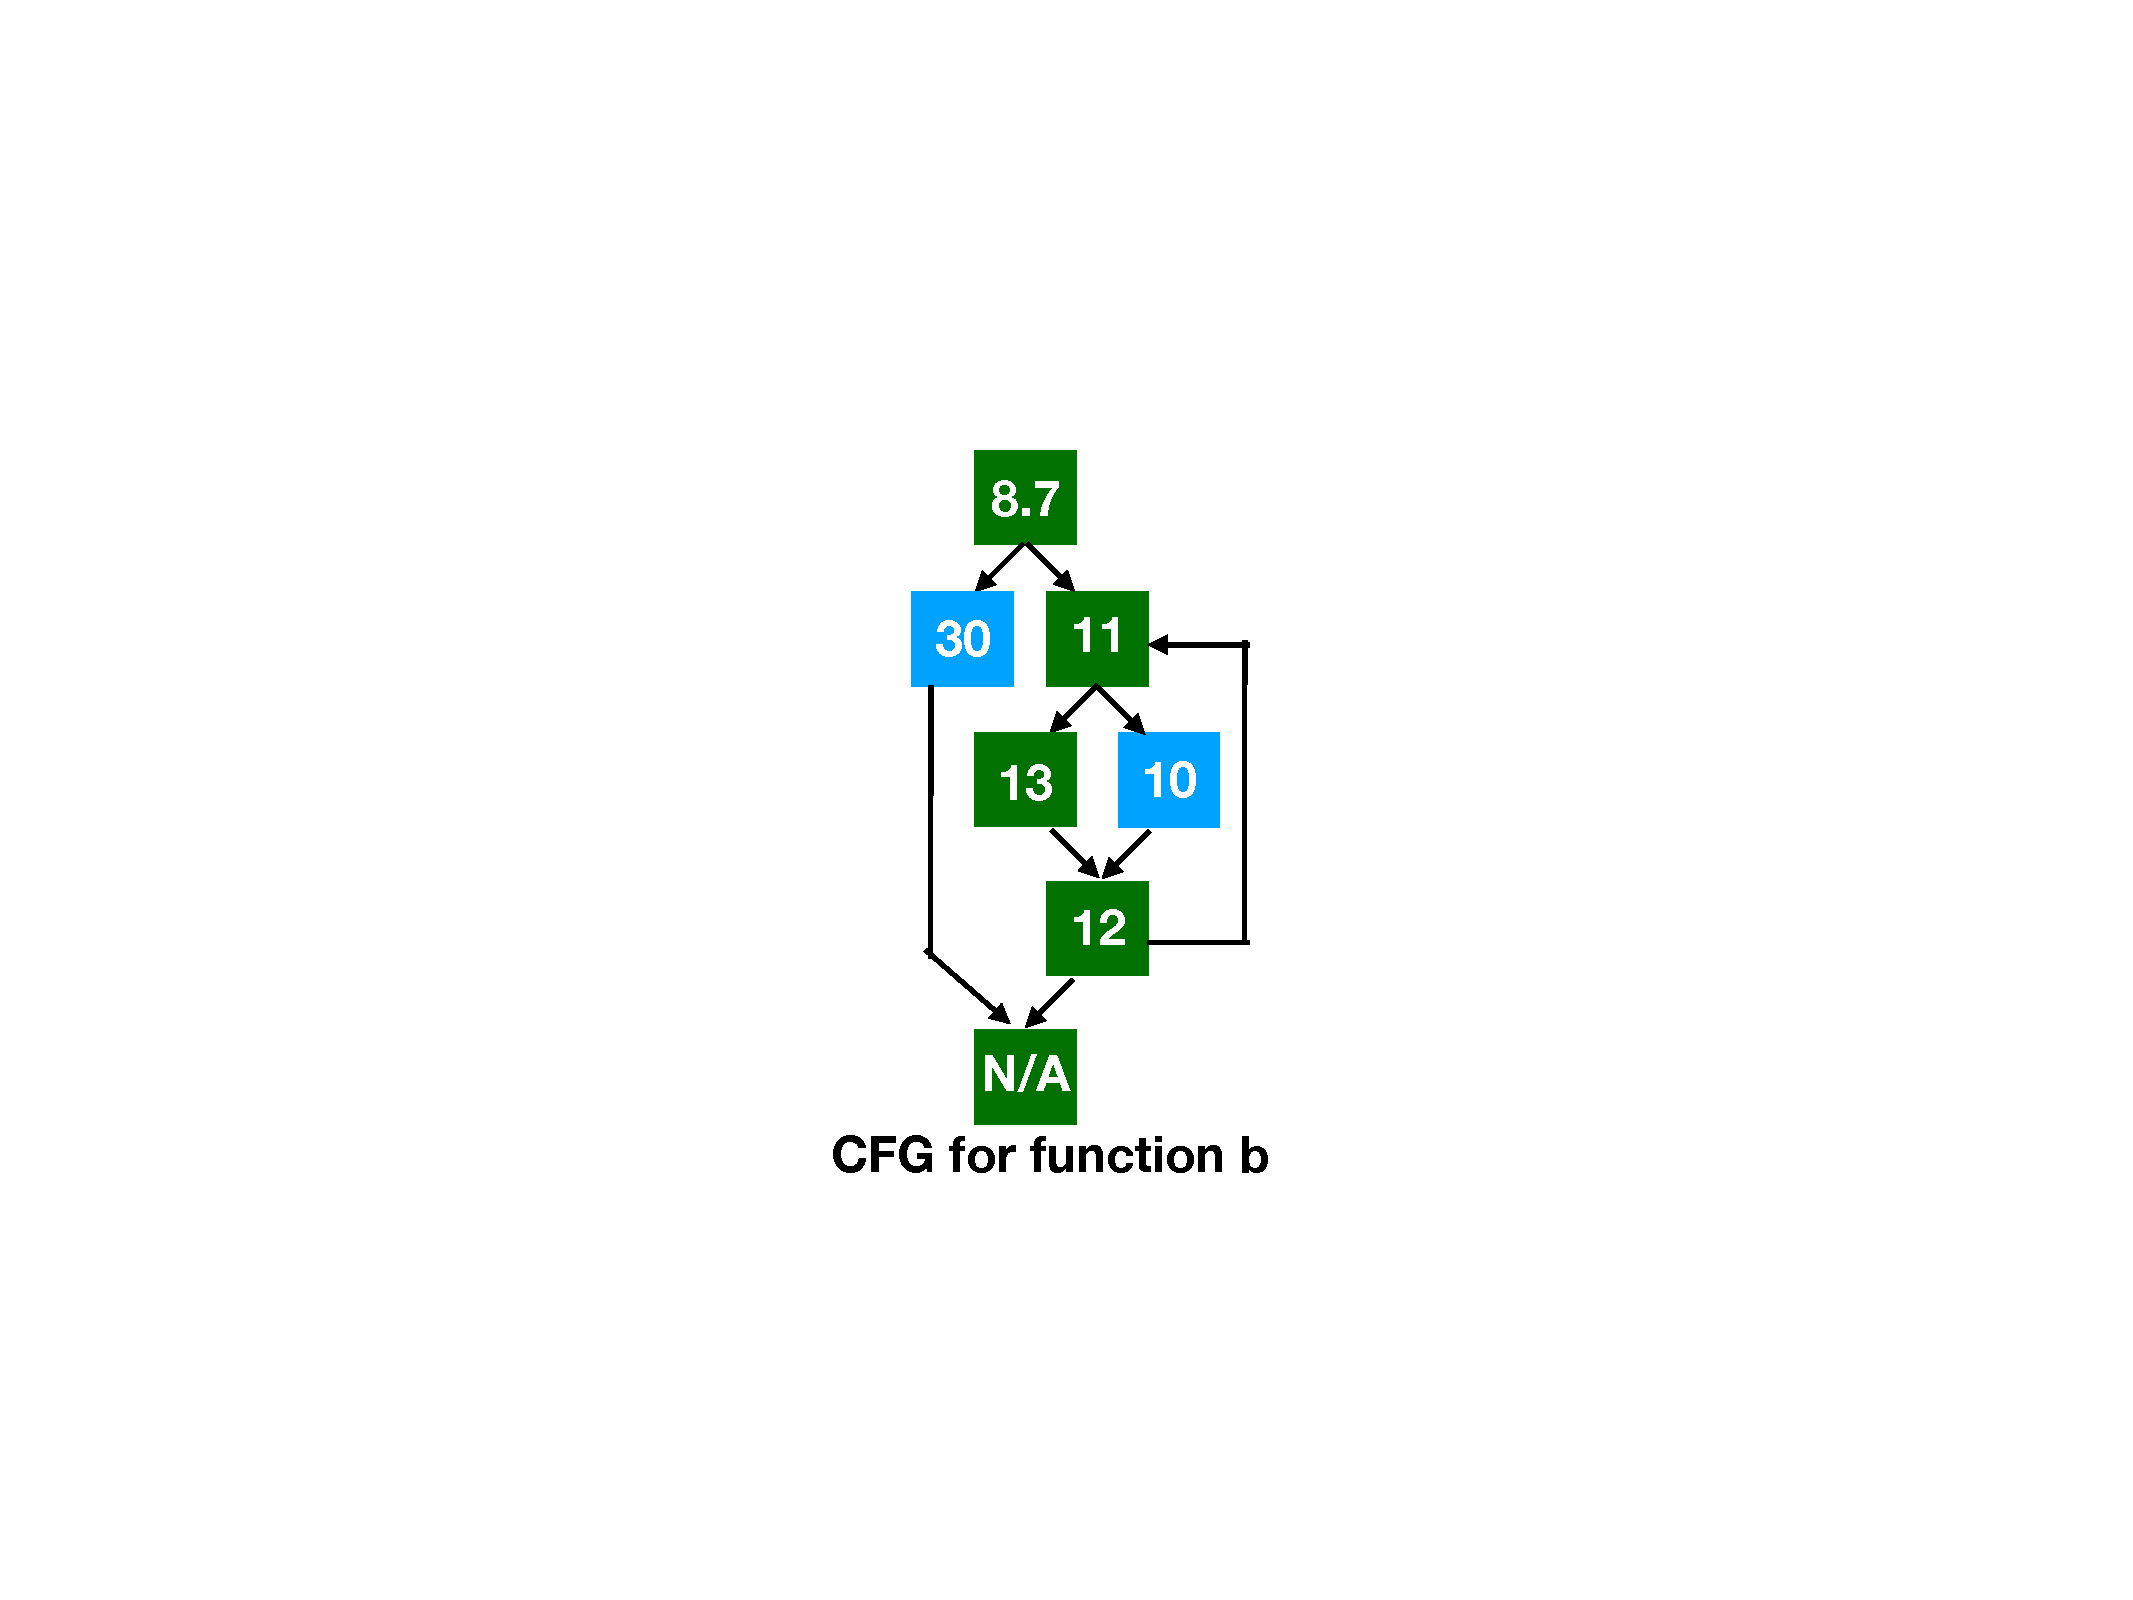
\includegraphics[width=3.0cm]{pic/CFG_4.pdf} }
            \only<3>{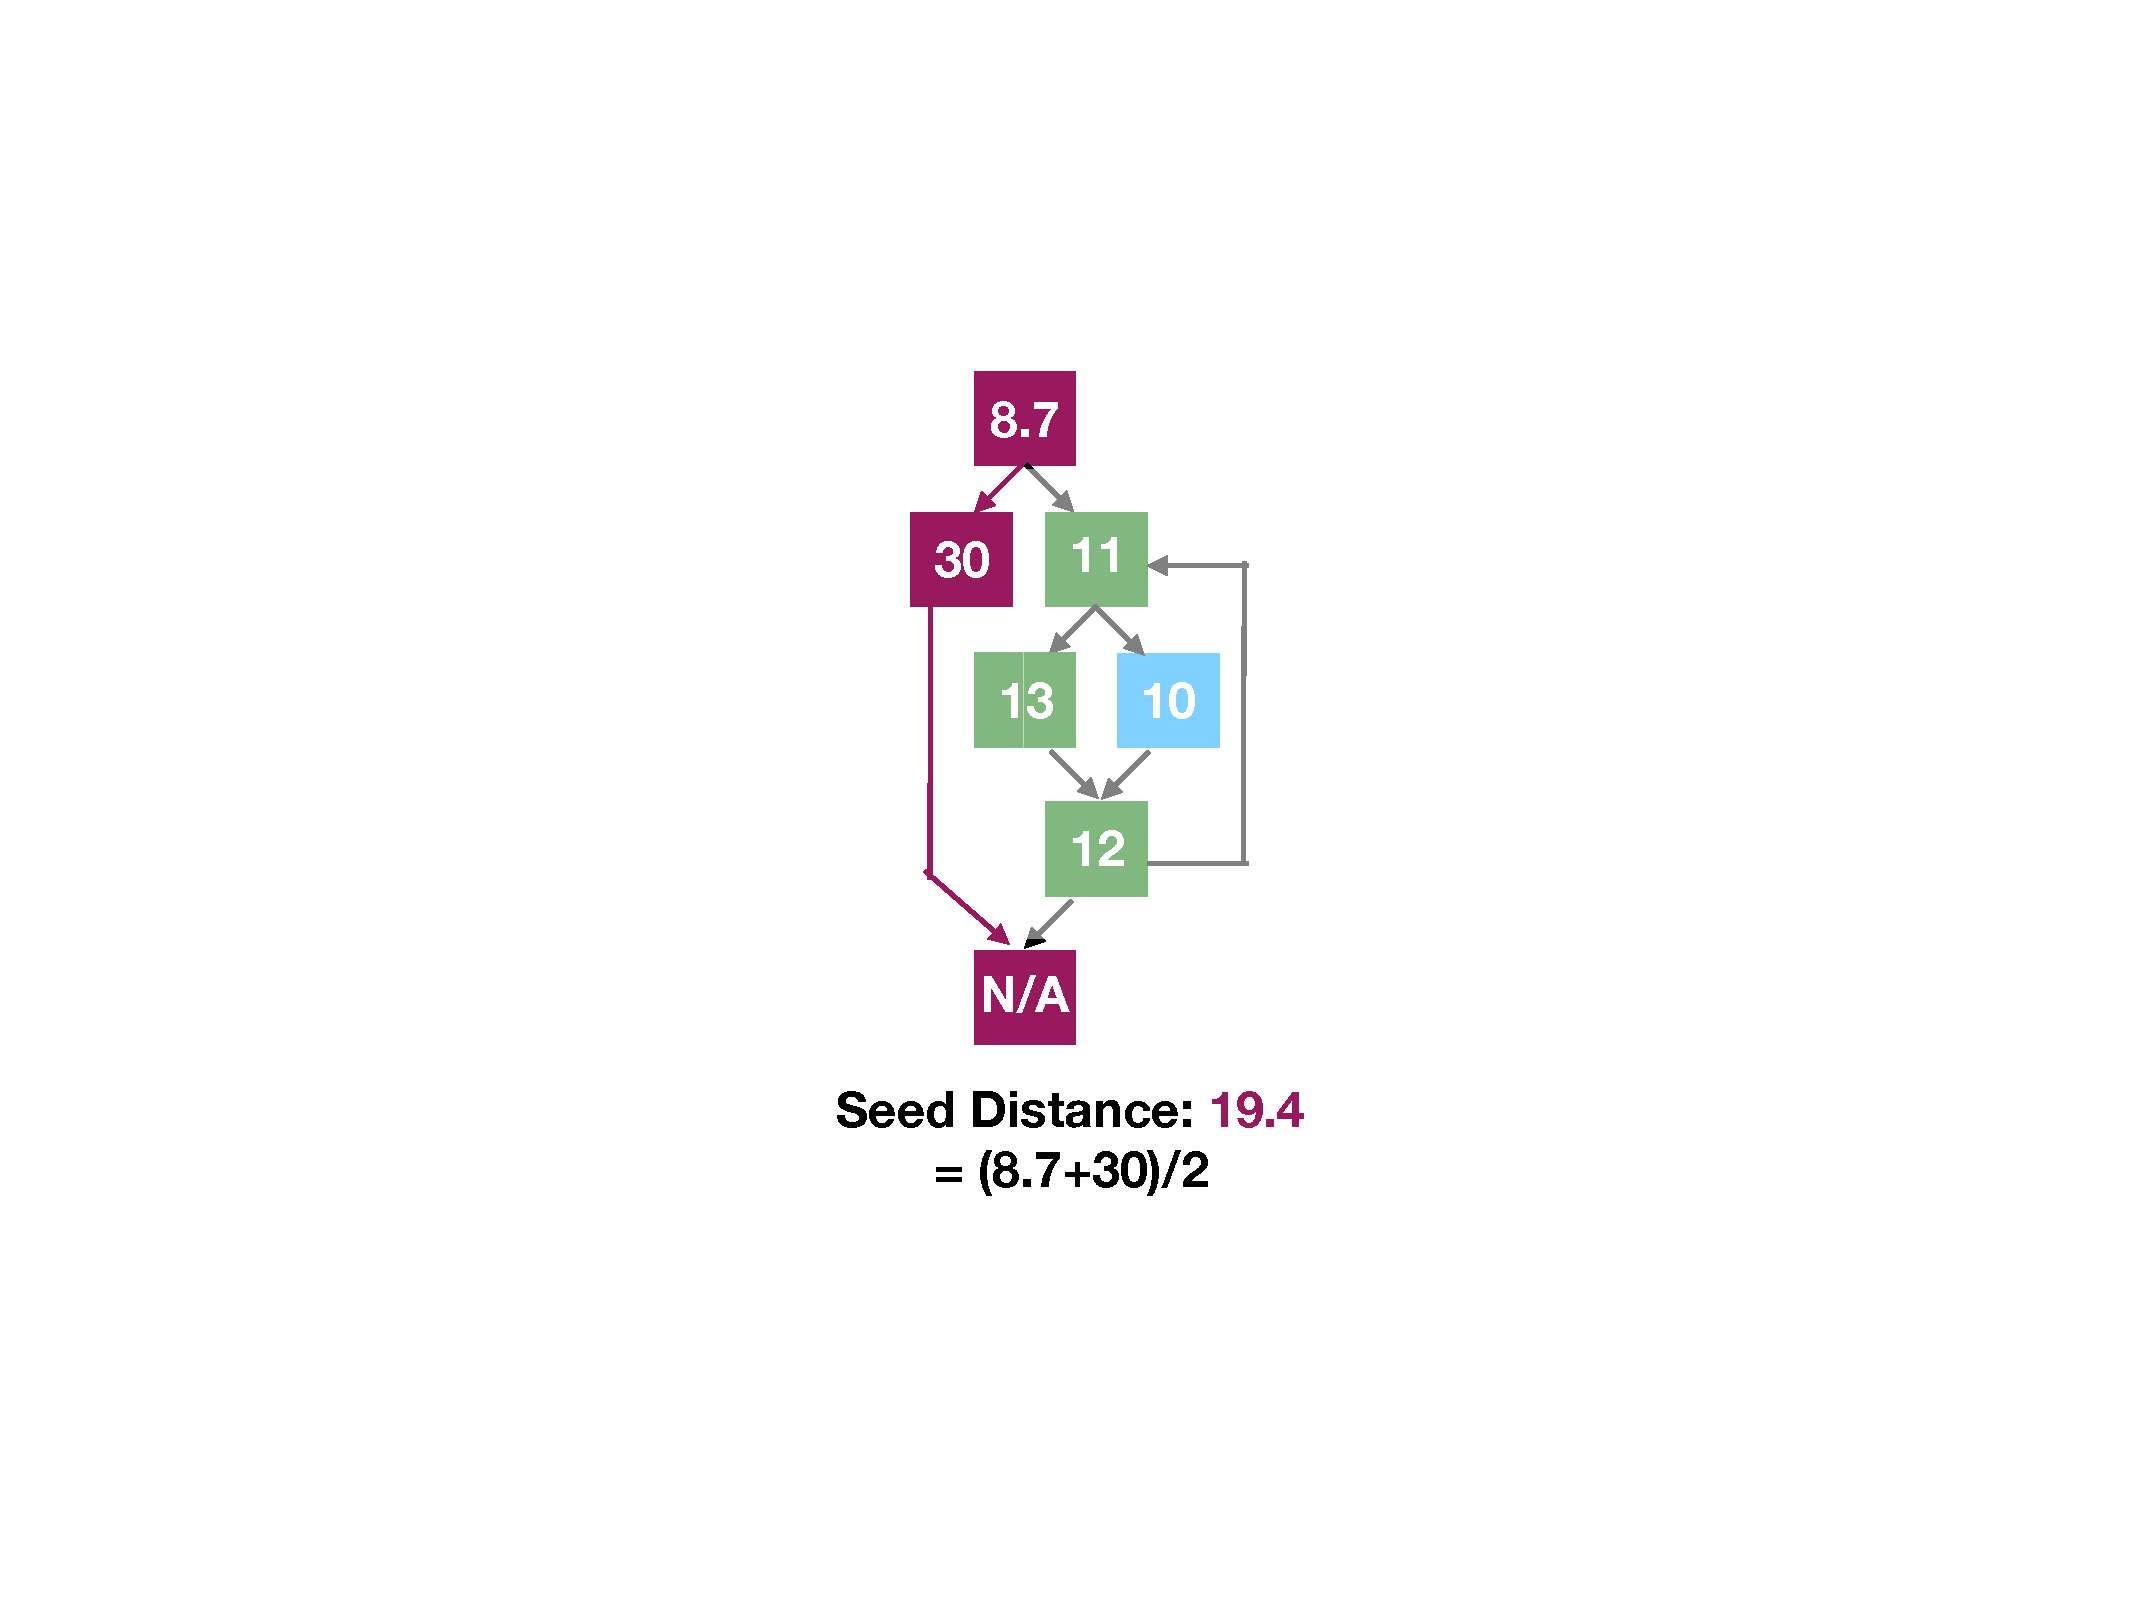
\includegraphics[width=3.5cm]{pic/CFG_5.pdf} }
            \only<4>{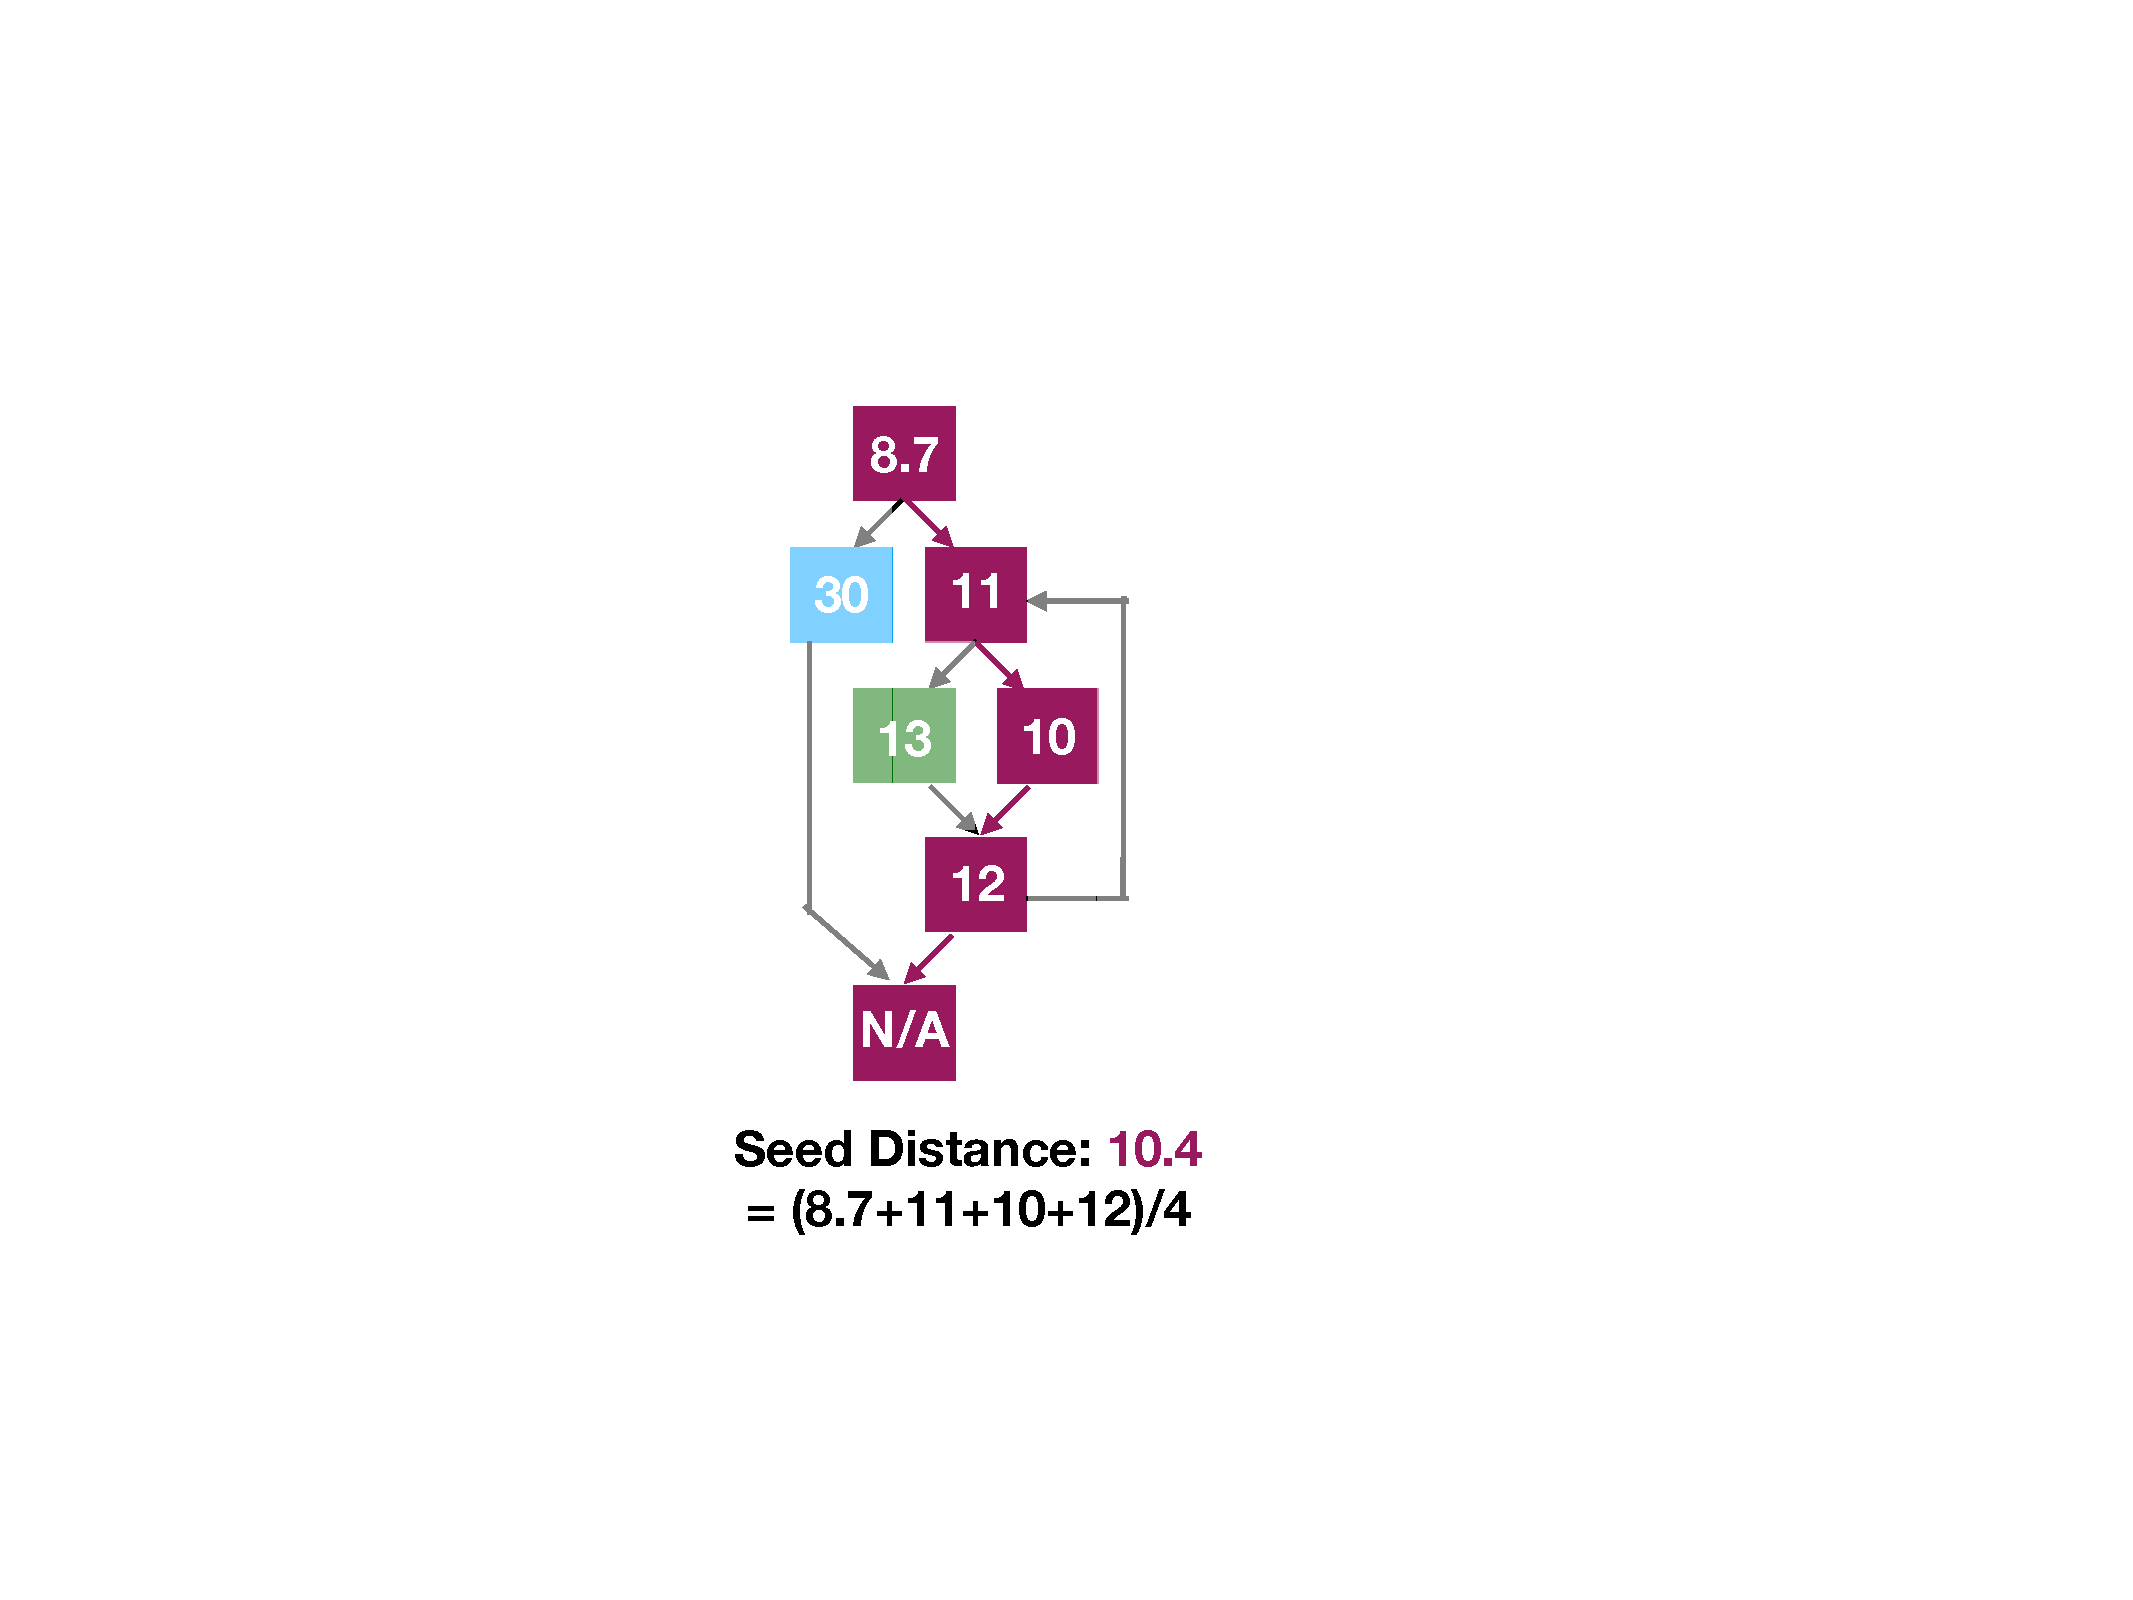
\includegraphics[width=3.5cm]{pic/CFG_6.pdf} }
       \end{minipage} 
    }
    \only<5>{
        \textbf{\structure{Directed Fuzzing } as \textcolor{deepgreen}{Optimisation Problem}}
        \begin{itemize}
            \item \textbf{Directed} Greybox Fuzzing
              \begin{itemize}
                \item [--] Assign \textbf{\textcolor{deepred}{more energy}} to seeds that are \textbf{\textcolor{deepred}{closer}} to the given targets
                \item [--] energy:The number of fuzz generated for a seed s is also called the energy of s.
              \end{itemize}
            \item \textbf{Simulated Annealing}
            \begin{itemize}
                \item [--]To avoid \textbf{\textcolor{deepred}{local minimum}} rather than \textbf{\textcolor{deepgreen}{global minimum}} distance
                \item [--]\textbf{Sometimes} assign \textbf{\textcolor{deepred}{more energy}} to \textbf{\textcolor{deepblue}{further-away}} seeds
            \end{itemize}  
            \item \textbf{\textit{Exploration} vs \textit{Exploitation}} 
            \begin{itemize}
                \item [--]\textbf{Exploration} phase:\\
                    Energy of \textbf{\textcolor{deepred}{closer}} seeds similar to energy of \textbf{\textcolor{deepblue}{further-away}} seeds
                \item [--]\textbf{Exploitation} phase:\\
                    - Energy of \textbf{\textcolor{deepred}{closer}} seeds is assigned  to be \textbf{\textcolor{deepred}{higher}} and higher\\
                    - Energy of \textbf{\textcolor{deepblue}{further-away}} seeds is assigned to be \textbf{\textcolor{deepblue}{lower}} and lower
            \end{itemize}  
         \end{itemize}
    }
    \only<6>
    {
        \textbf{\structure{Directed Fuzzing } as \textcolor{deepgreen}{Optimisation Problem}}
        \begin{itemize}
            \item \textbf{Temperature} 
            \\ $T \in [0,1]$ specifies “importance” of distance.
            \begin{itemize}
                \item [--]normalized seed distance
                \\$$\widetilde{d}(s,T_b)=\frac{d(s,T_b)-\text{minD}}{\text{maxD}-\text{minD}} \in [0,1]$$
                \item [--]At T=1, \textbf{exploration} (normal AFL)
                \item [--]At T=0, \textbf{exploitation} (gradient descent)
            \end{itemize}  
            \item \textbf{Cooling schedule} :controls (global) temperature
            \begin{itemize}
                \item [--]Classically, exponential cooling.
            \end{itemize} 
         \end{itemize} 
    }
    \only<7-9>{
        \textbf{ Integrating Simulated Annealing as power schedule}
        \begin{minipage}[t]{0.45\linewidth}
            \vspace{0pt} 
            \begin{itemize}
                \item  In the beginning (t = 0min), assign the \textbf{\textcolor{violet}{same energy}} to \textbf{\textcolor{violet}{all seeds}}
                \onslide<8-9>{ \item  Later (t=10min), assign\textbf{\textcolor{brown}{ a bit more energy}} to seeds that are \textbf{\textcolor{brown}{closer}}}
                \onslide<9>{ \item At exploitation (t=80min), assign \textbf{\textcolor{deepred}{maximal energy}} to seeds that are \textbf{\textcolor{red}{closest}}}
             \end{itemize} 
        \end{minipage}
        \begin{minipage}[t]{0.5\linewidth}
            \vspace{0pt}
            \centering
            \only<7>{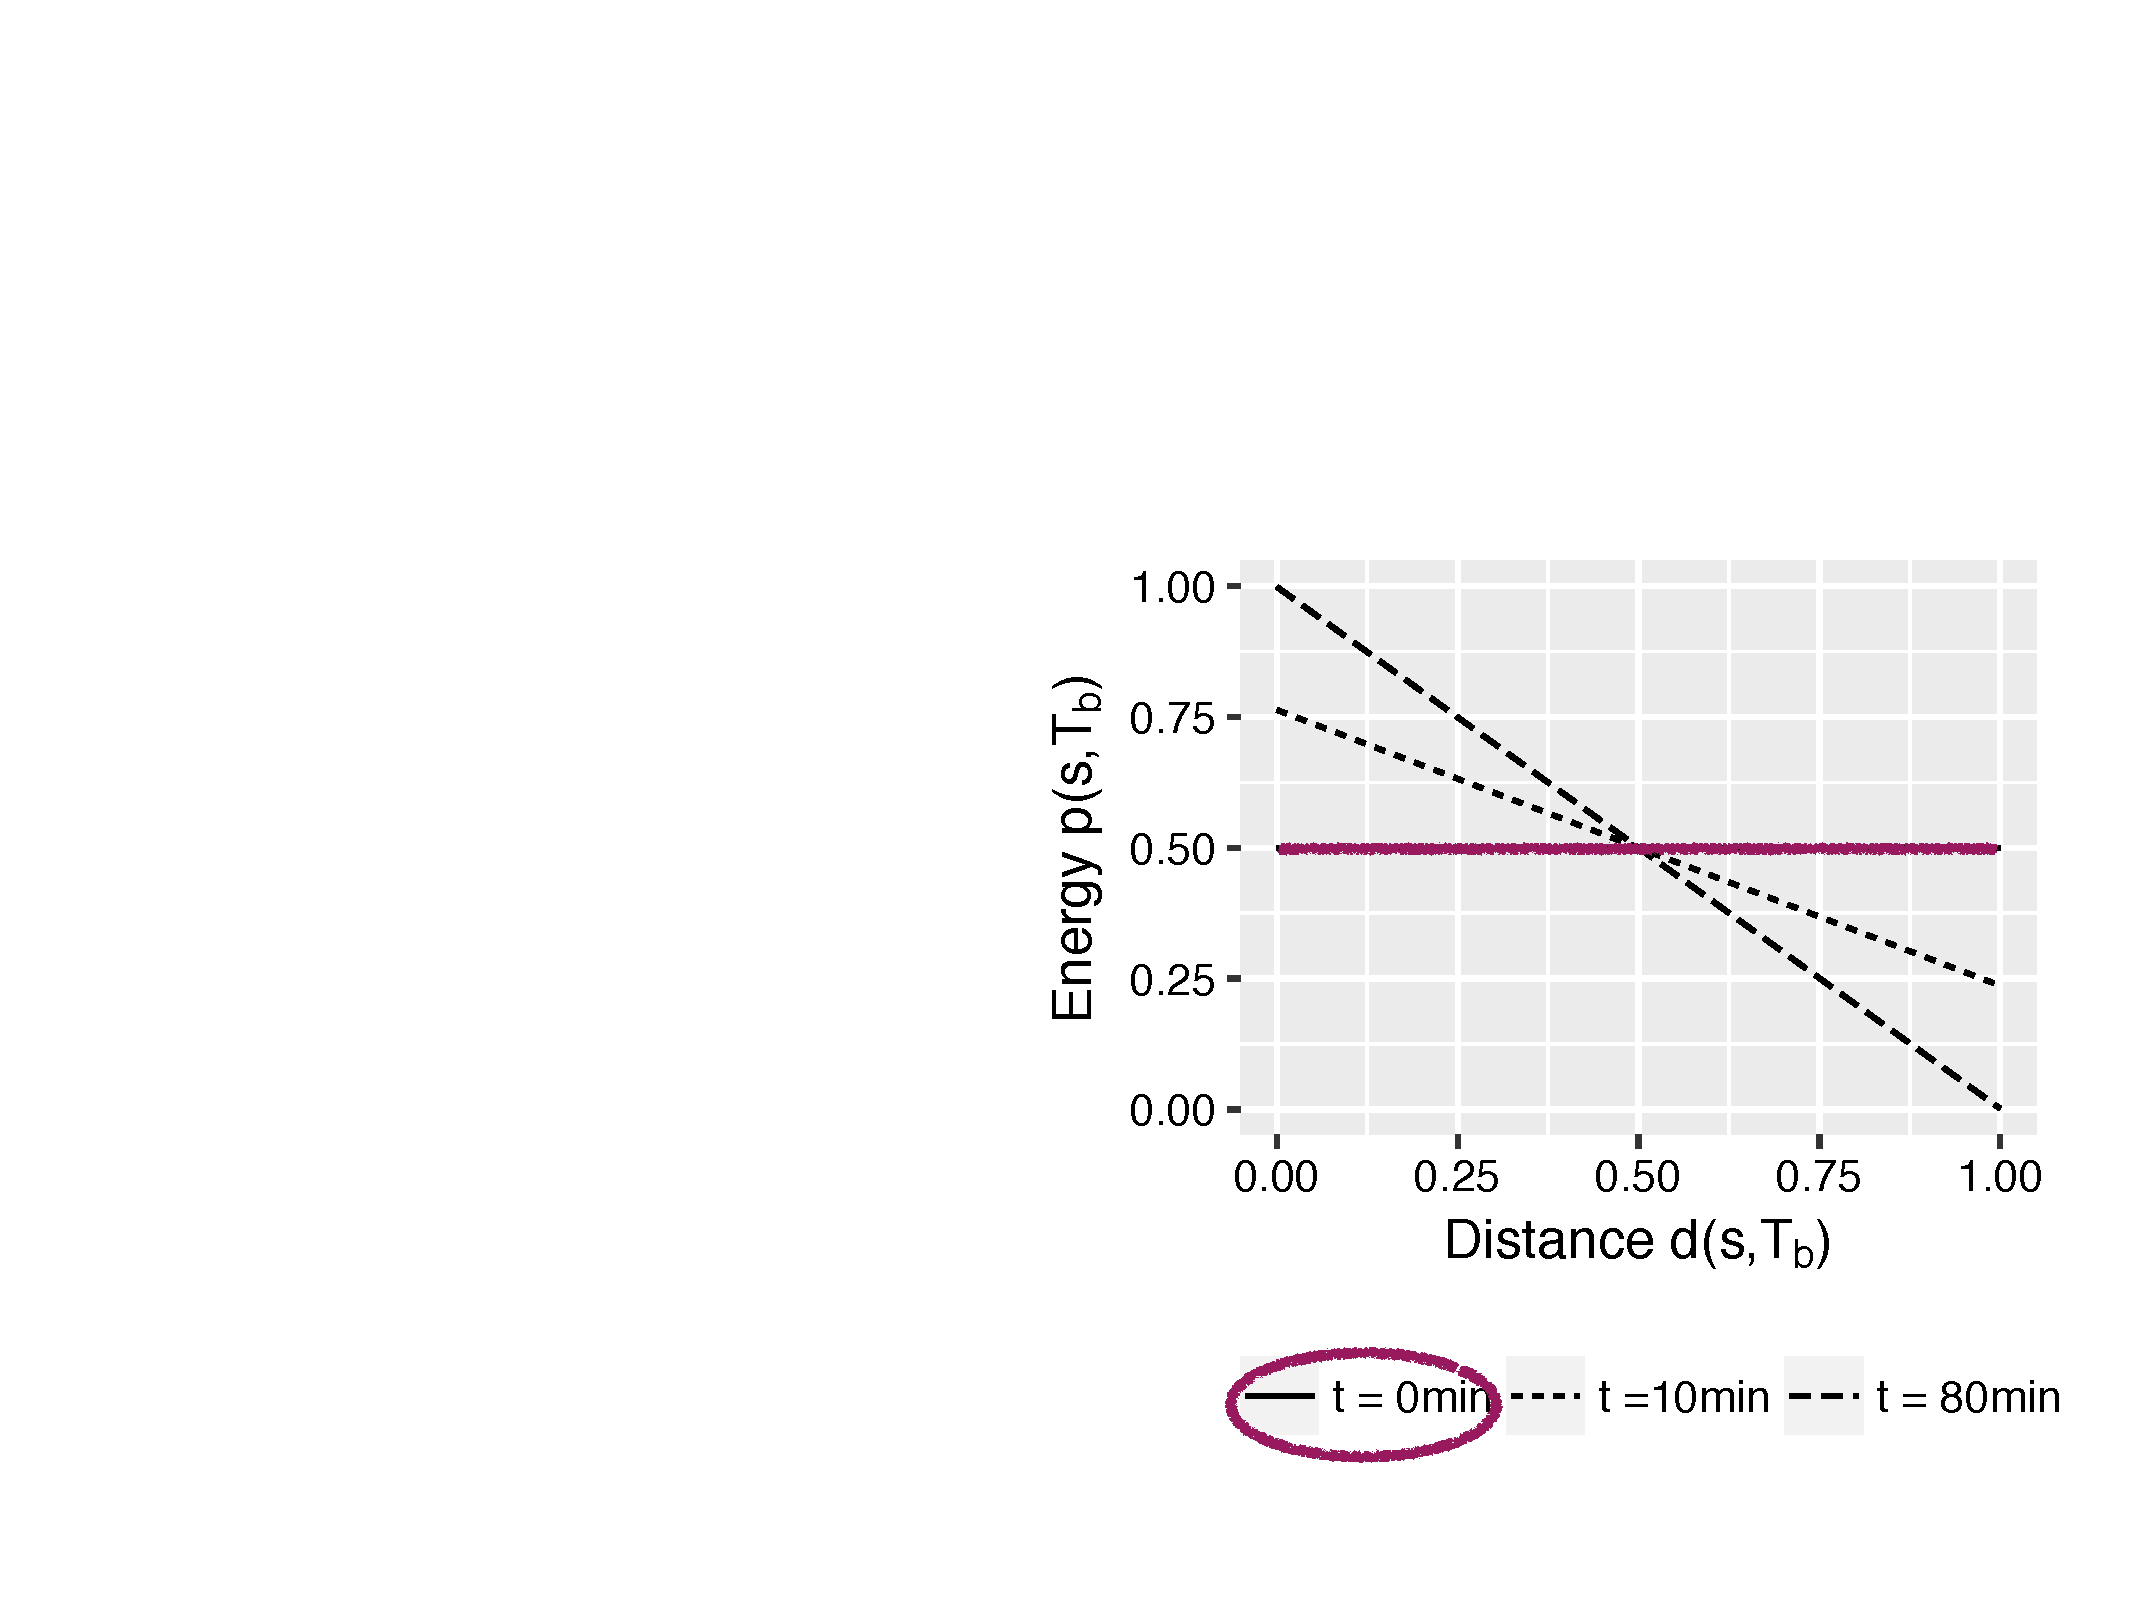
\includegraphics[width=5.6cm]{pic/SA_1.pdf}}
            \only<8>{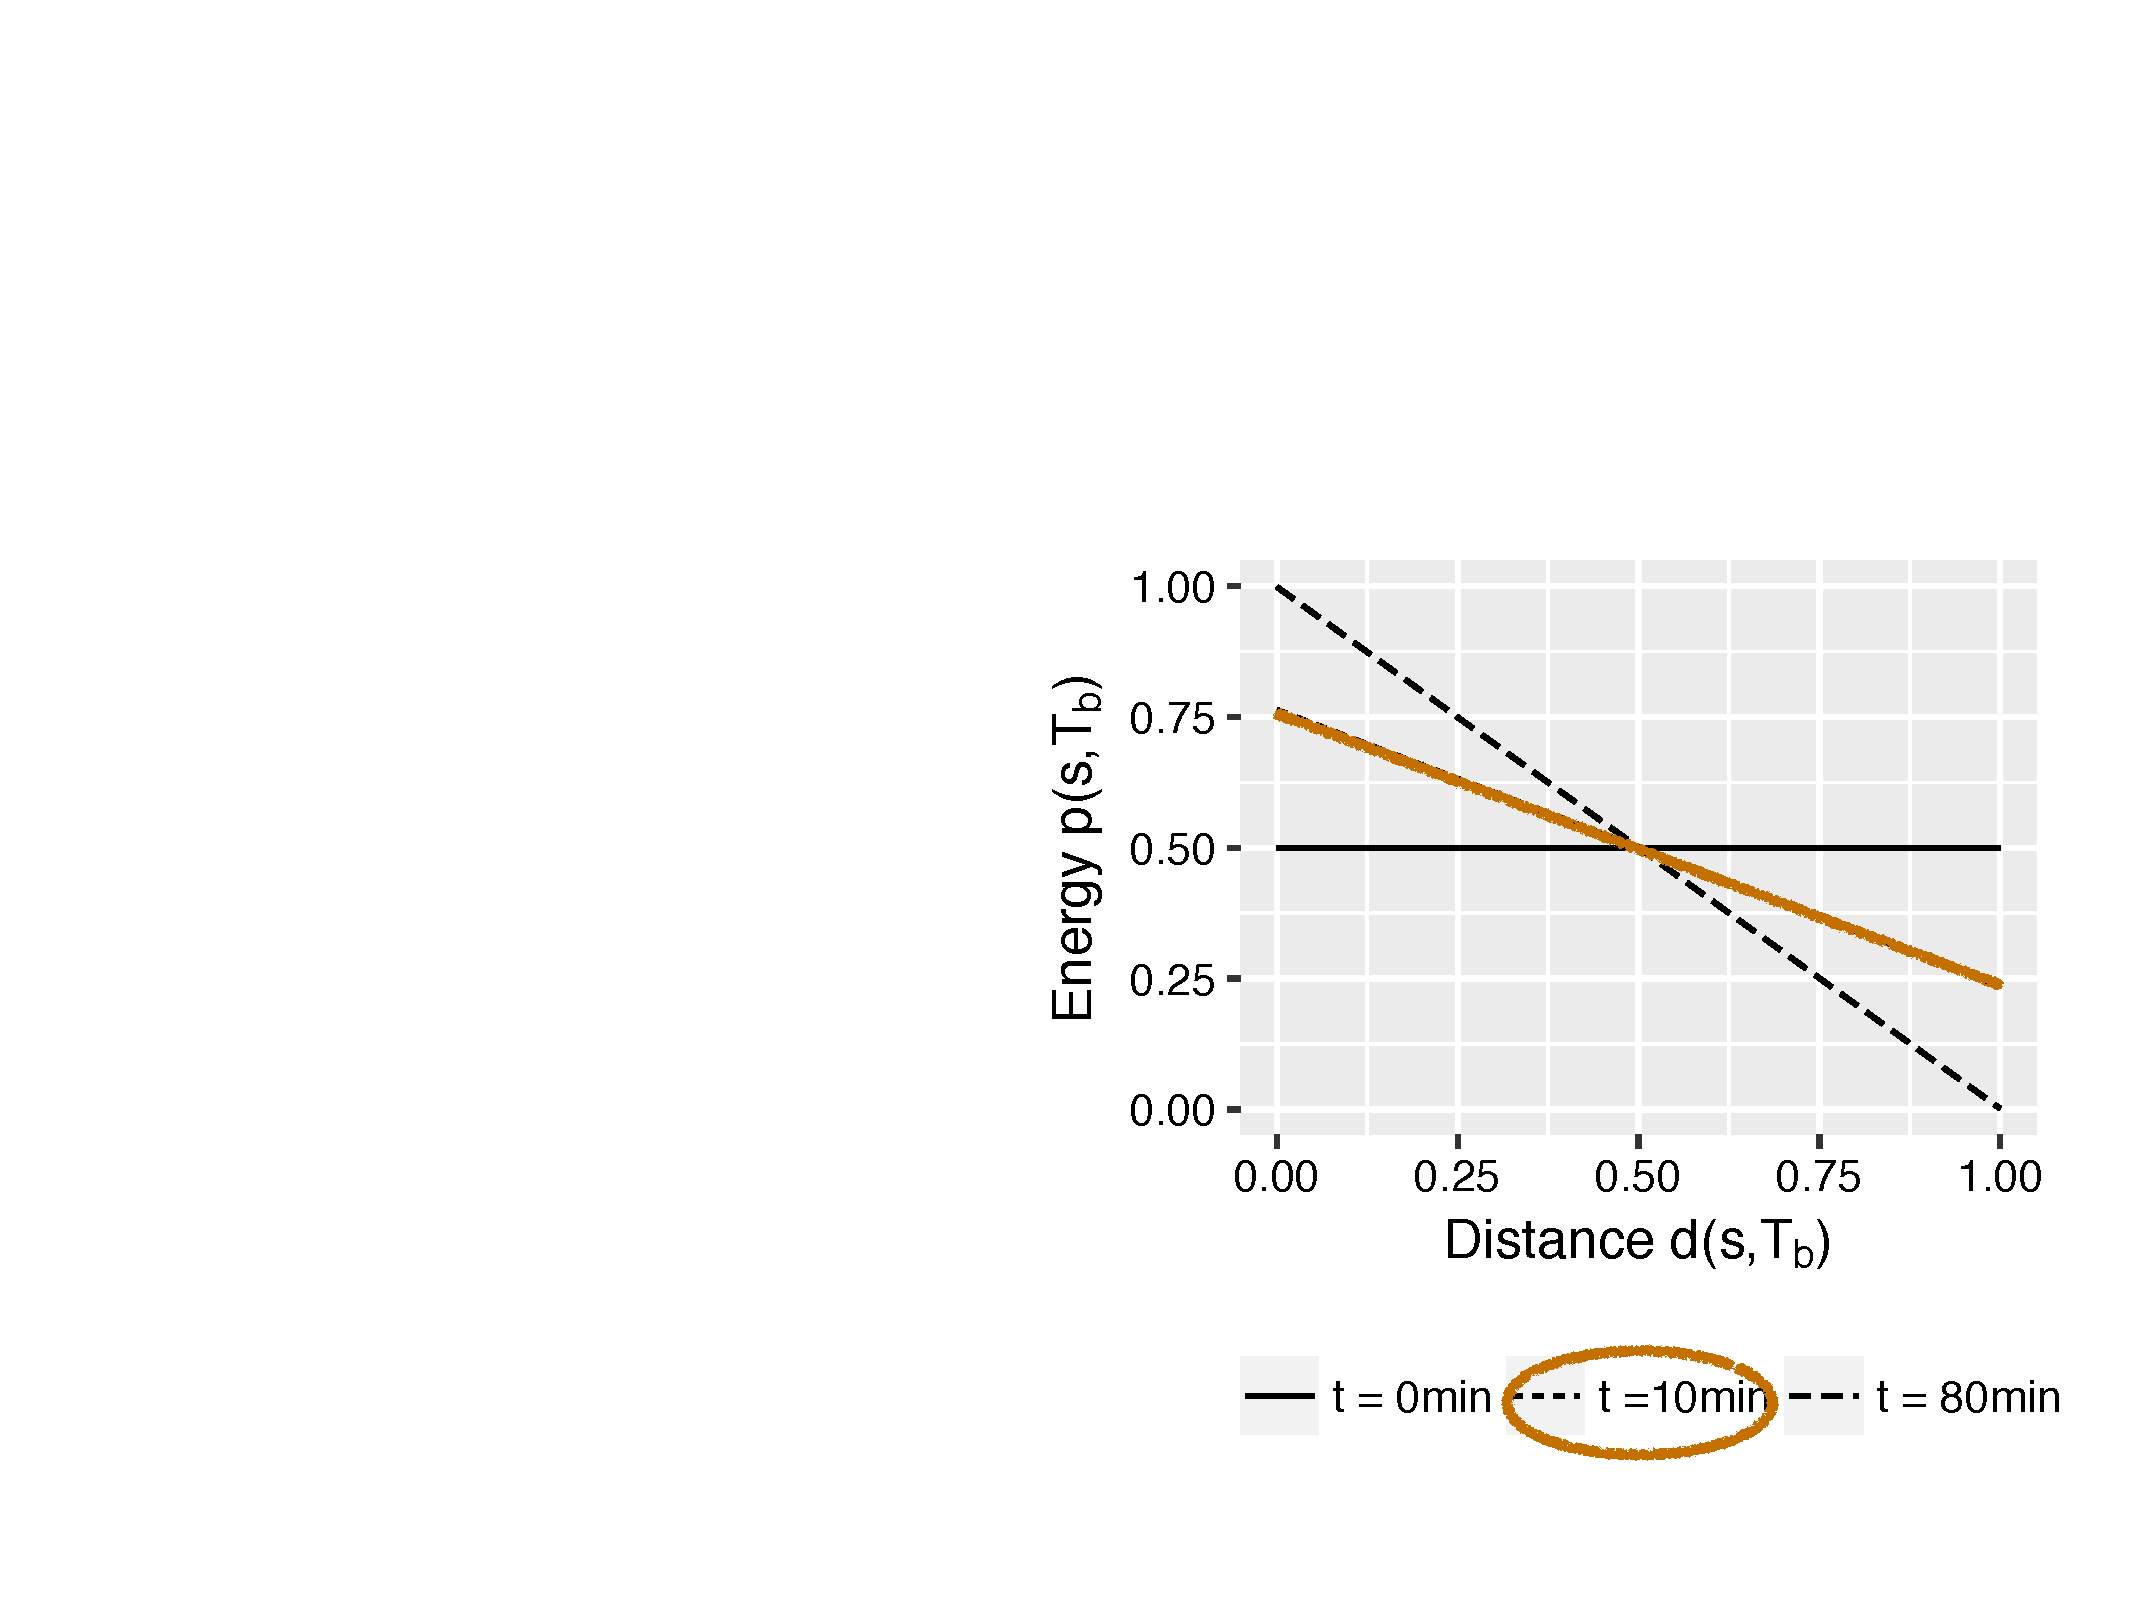
\includegraphics[width=5.6cm]{pic/SA_2.pdf}}  
            \only<9>{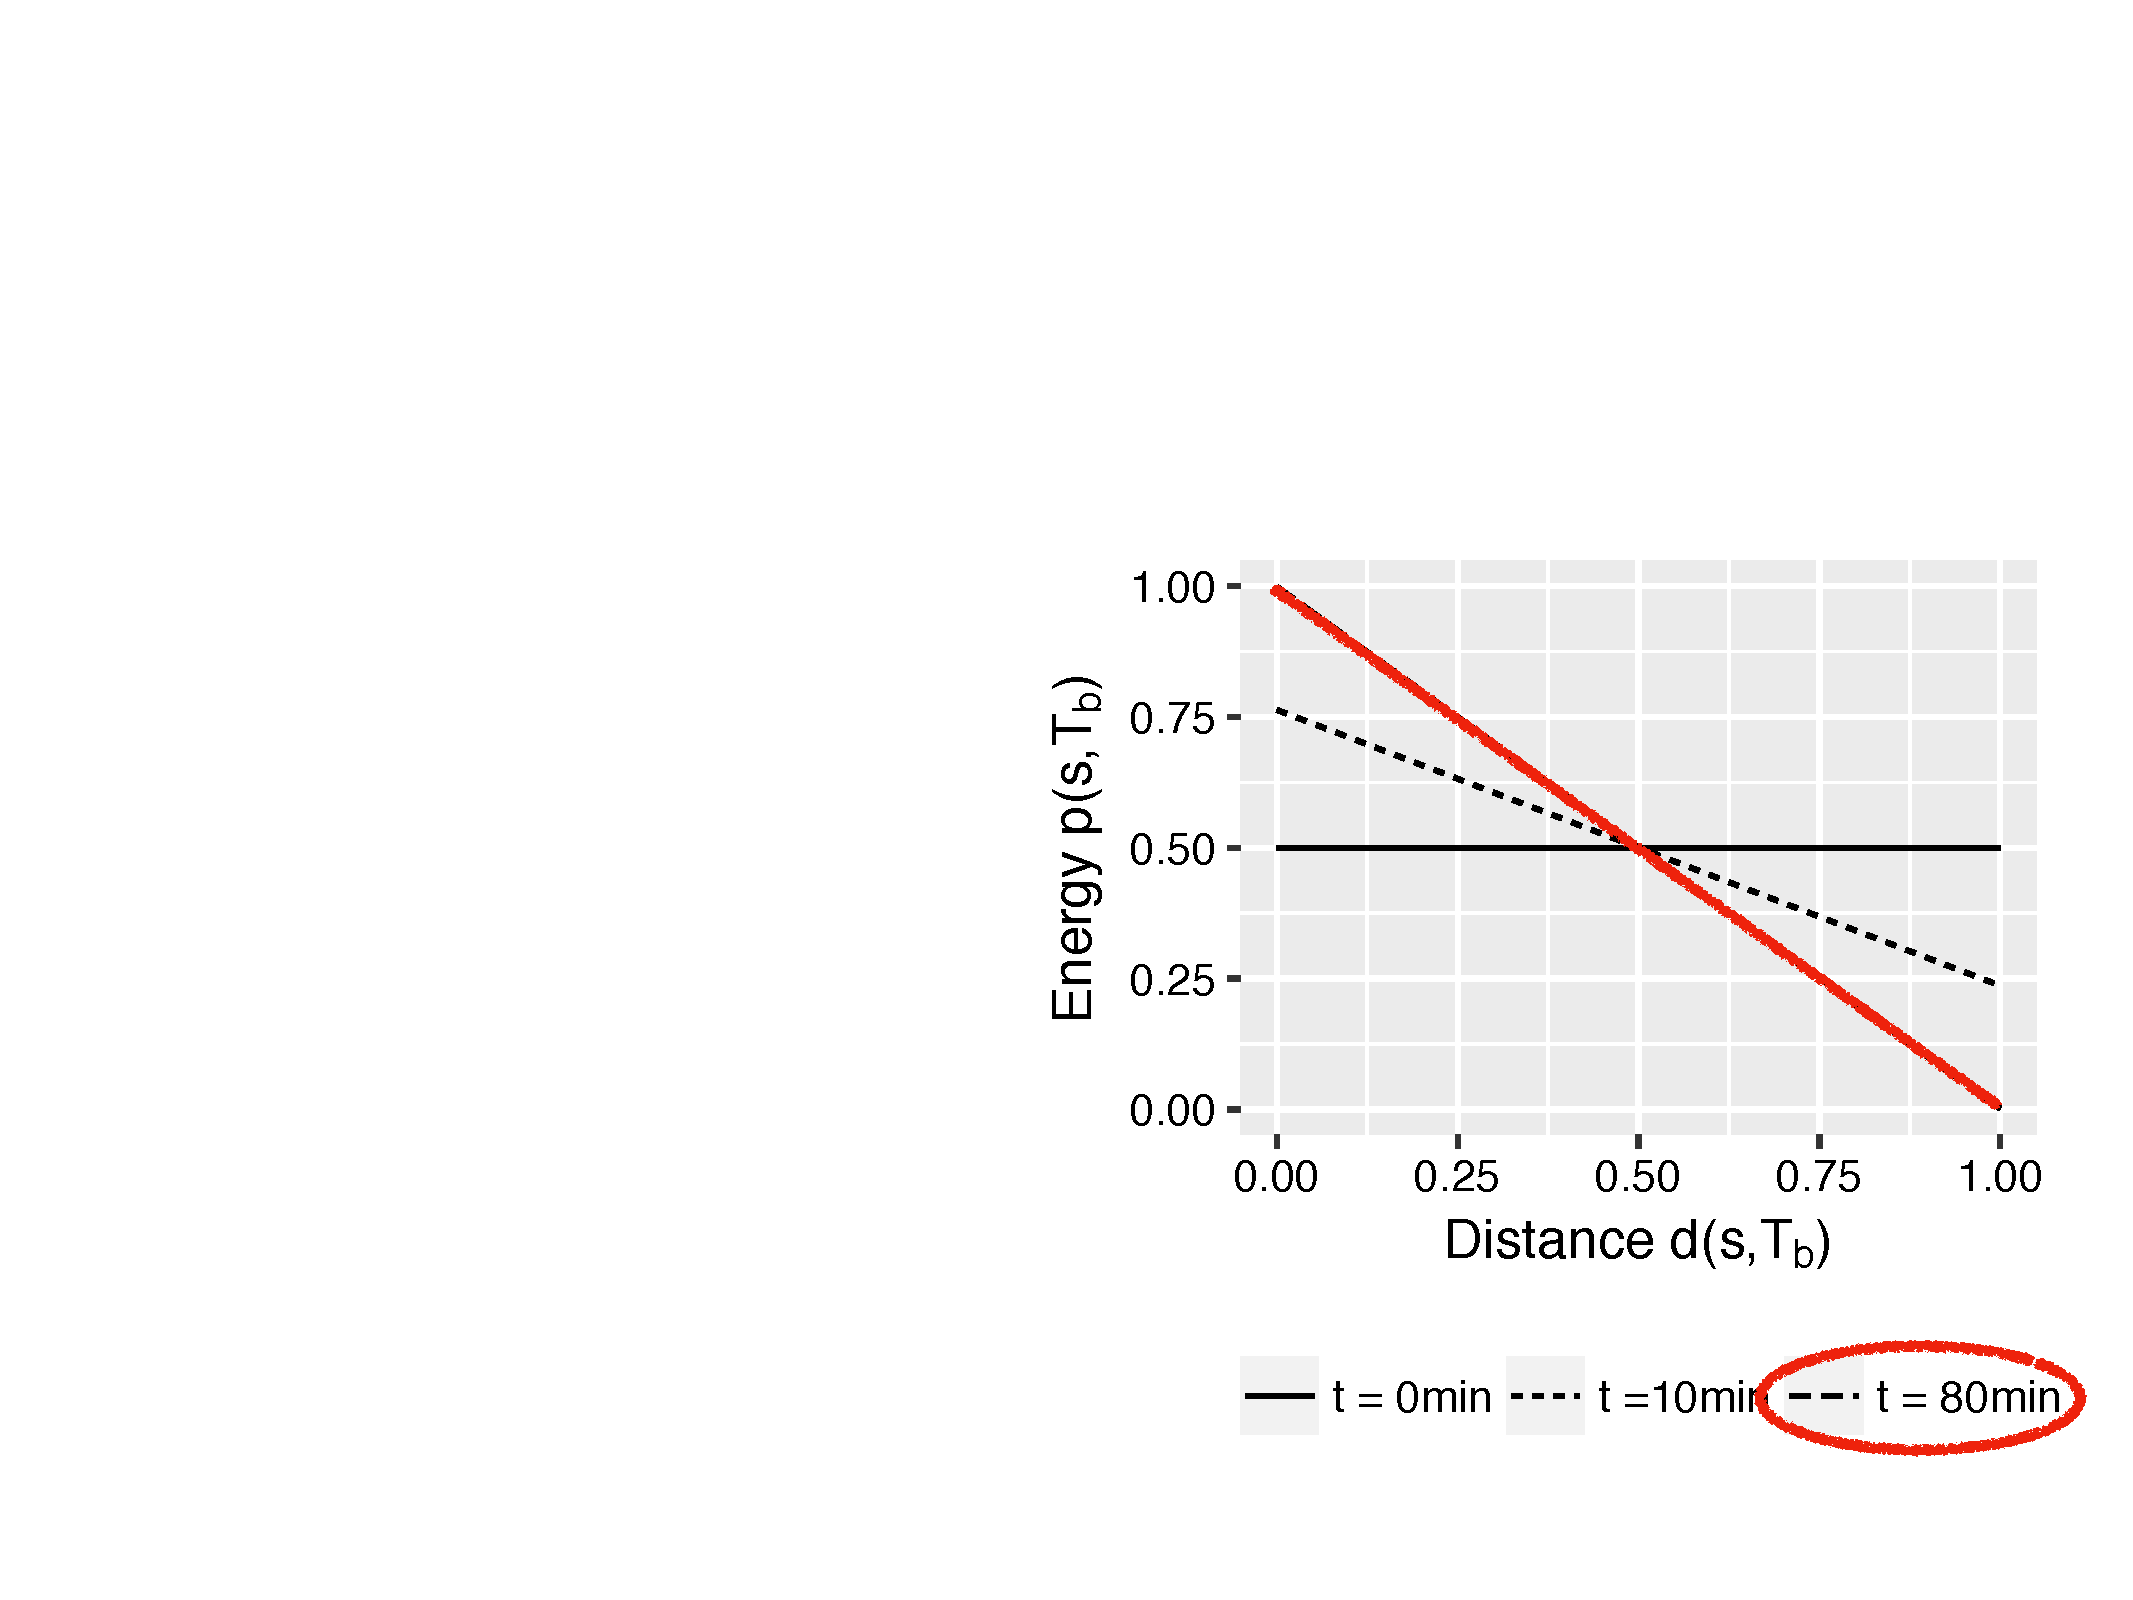
\includegraphics[width=5.6cm]{pic/SA_3.pdf}}  
        \end{minipage} 
    }
    \only<10>{
        \begin{algorithm}[H]
            \footnotesize
            \DontPrintSemicolon
            \SetKwSty{algokeywordsty}
            \SetFuncSty{algofuncsty}
            \SetDataSty{algodatasty}
            \SetArgSty{algoargsty}
            \SetCommentSty{algocmtsty}
            \SetKw{break}{break}
            \SetKw{not}{not}
            \SetKwFunction{graphextractor}{\textsc{GraphExt}}
            \SetKwFunction{bbdistance}{\textsc{DisCalcu}}  
            \SetKwFunction{select}{\textsc{Dequeue}}
            \SetKwFunction{assinenergy}{\textsc{AssinEnergy}}
            \SetKwFunction{mutation}{\textsc{Mutation}}
            \SetKwFunction{execution}{\textsc{Execution}}
            \SetKwFunction{IsIntersting}{\textsc{IsIntersting}}
            \SetKwFunction{evaluateseed}{\textsc{SeedDis}}
            \SetKwFunction{sortinsert}{Enqueue}
            % \SetKwData{crashseeds}{$\seeds_{\text{\emoji{boom}}}$}
            \SetKwData{crashseeds}{$\seeds^\prime$} 
            \SetKwData{seedqueue}{$\textit{SeedQueue}$}  
            \SetKwData{Graph}{$\textit{Graphs}$}  
            \SetKwData{BBdis}{$\textit{BBdistance}$} 
            \SetKwData{newseed}{$\seed^\prime$}   
            \SetKwData{energy}{$\textit{e}$}
            \SetKwData{trace}{$\textit{trace}$} 
            \SetKwData{distance}{$\textit{distance}$}   
            \KwIn{\seeds\tcp{a finite set of seeds}}
            \KwIn{\targets\tcp{a finite set of targer sits}} 
            \KwOut{\crashseeds \tcp{a finite set of buggy seeds}}
            $\crashseeds\gets \varnothing$\; 
            $\seedqueue \gets \seeds$\;
            \Graph $\gets \graphextractor{\sourcecode}$\;
            \BBdis $\gets \bbdistance{\targets,\Graph}$\;
            \While {$!siganl \land \currtime < \timeout$}{
              \seed$\gets \select{\seedqueue}$\;
              $\trace \gets \execution{\seed}$\; 
              $\distance \gets \evaluateseed{\trace, \BBdis} $\;
              \energy $\gets \assinenergy{\seed, \currtime, \distance}$\;
               \For{$\textit{i}\gets 1$ \KwTo $\energy$}
               {
                $\newseed \gets \mutation{\seed}$\;      
                \HiLi\lIf{\newseed crashes}{$\crashseeds \gets \crashseeds \cup \newseed $}
                \HiLi\lIf{\IsIntersting{\newseed}}{    
                    $\sortinsert{\newseed,\seedqueue} $ 
                }
               }
            }
            \Return{\crashseeds}\;
        \end{algorithm} 
    }
\end{frame}



\section{Work}

% \begin{frame}{排版举例}
%     \begin{exampleblock}{无编号公式} % 加 * 
%         \begin{equation*}
%             J(\theta) = \mathbb{E}_{\pi_\theta}[G_t] = \sum_{s\in\mathcal{S}} d^\pi (s)V^\pi(s)=\sum_{s\in\mathcal{S}} d^\pi(s)\sum_{a\in\mathcal{A}}\pi_\theta(a|s)Q^\pi(s,a)
%         \end{equation*}
%     \end{exampleblock}
%     \begin{exampleblock}{多行多列公式\footnote{如果公式中有文字出现,请用 $\backslash$mathrm\{\} 或者 $\backslash$text\{\} 包含,不然就会变成 $clip$,在公式里看起来比 $\mathrm{clip}$ 丑非常多。}}
%         % 使用 & 分隔
%         \begin{align}
%             Q_\mathrm{target}&=r+\gamma Q^\pi(s^\prime, \pi_\theta(s^\prime)+\epsilon)\\
%             \epsilon&\sim\mathrm{clip}(\mathcal{N}(0, \sigma), -c, c)\nonumber
%         \end{align}
%     \end{exampleblock}
% \end{frame}

% \begin{frame}
%     \begin{exampleblock}{编号多行公式}
%         % Taken from Mathmode.tex
%         \begin{multline}
%             A=\lim_{n\rightarrow\infty}\Delta x\left(a^{2}+\left(a^{2}+2a\Delta x+\left(\Delta x\right)^{2}\right)\right.\label{eq:reset}\\
%             +\left(a^{2}+2\cdot2a\Delta x+2^{2}\left(\Delta x\right)^{2}\right)\\
%             +\left(a^{2}+2\cdot3a\Delta x+3^{2}\left(\Delta x\right)^{2}\right)\\
%             +\ldots\\
%             \left.+\left(a^{2}+2\cdot(n-1)a\Delta x+(n-1)^{2}\left(\Delta x\right)^{2}\right)\right)\\
%             =\frac{1}{3}\left(b^{3}-a^{3}\right)
%         \end{multline}
%     \end{exampleblock}
% \end{frame}


% \begin{frame}[fragile]{\LaTeX{} 常用命令}
%     \begin{exampleblock}{命令}
%         \centering
%         \footnotesize
%         \begin{tabular}{llll}
%             \cmd{chapter} & \cmd{section} & \cmd{subsection} & \cmd{paragraph} \\
%             章 & 节 & 小节 & 带题头段落 \\\hline
%             \cmd{centering} & \cmd{emph} & \cmd{verb} & \cmd{url} \\
%             居中对齐 & 强调 & 原样输出 & 超链接 \\\hline
%             \cmd{footnote} & \cmd{item} & \cmd{caption} & \cmd{includegraphics} \\
%             脚注 & 列表条目 & 标题 & 插入图片 \\\hline
%             \cmd{label} & \cmd{cite} & \cmd{ref} \\
%             标号 & 引用参考文献 & 引用图表公式等\\\hline
%         \end{tabular}
%     \end{exampleblock}
%     \begin{exampleblock}{环境}
%         \centering
%         \footnotesize
%         \begin{tabular}{lll}
%             \env{table} & \env{figure} & \env{equation}\\
%             表格 & 图片 & 公式 \\\hline
%             \env{itemize} & \env{enumerate} & \env{description}\\
%             无编号列表 & 编号列表 & 描述 \\\hline
%         \end{tabular}
%     \end{exampleblock}
% \end{frame}

% \begin{frame}[fragile]{\LaTeX{} 环境命令举例}
%     \begin{minipage}{0.5\linewidth}
% \begin{lstlisting}[language=TeX]
% \begin{itemize}
%   \item A \item B
%   \item C
%   \begin{itemize}
%     \item C-1
%   \end{itemize}
% \end{itemize}
% \end{lstlisting}
%     \end{minipage}\hspace{1cm}
%     \begin{minipage}{0.3\linewidth}
%         \begin{itemize}
%             \item A
%             \item B
%             \item C
%             \begin{itemize}
%                 \item C-1
%             \end{itemize}
%         \end{itemize}
%     \end{minipage}
%     \medskip
%     \pause
%     \begin{minipage}{0.5\linewidth}
% \begin{lstlisting}[language=TeX]
% \begin{enumerate}
%   \item 巨佬 \item 大佬
%   \item 萌新
%   \begin{itemize}
%     \item[n+e] 瑟瑟发抖
%   \end{itemize}
% \end{enumerate}
% \end{lstlisting}
%     \end{minipage}\hspace{1cm}
%     \begin{minipage}{0.3\linewidth}
%         \begin{enumerate}
%             \item 巨佬
%             \item 大佬
%             \item 萌新
%             \begin{itemize}
%                 \item[n+e] 瑟瑟发抖
%             \end{itemize}
%         \end{enumerate}
%     \end{minipage}
% \end{frame}

% \begin{frame}[fragile]{\LaTeX{} 数学公式}
%     \begin{columns}
%         \begin{column}{.55\textwidth}
% \begin{lstlisting}[language=TeX]
% $V = \frac{4}{3}\pi r^3$

% \[
%   V = \frac{4}{3}\pi r^3
% \]

% \begin{equation}
%   \label{eq:vsphere}
%   V = \frac{4}{3}\pi r^3
% \end{equation}
% \end{lstlisting}
%         \end{column}
%         \begin{column}{.4\textwidth}
%             $V = \frac{4}{3}\pi r^3$
%             \[
%                 V = \frac{4}{3}\pi r^3
%             \]
%             \begin{equation}
%                 \label{eq:vsphere}
%                 V = \frac{4}{3}\pi r^3
%             \end{equation}
%         \end{column}
%     \end{columns}
%     \begin{itemize}
%         \item 更多内容请看 \href{https://zh.wikipedia.org/wiki/Help:数学公式}{\color{purple}{这里}}
%     \end{itemize}
% \end{frame}

% \begin{frame}[fragile]
%     \begin{columns}
%         \column{.6\textwidth}
% \begin{lstlisting}[language=TeX]
%     \begin{table}[htbp]
%       \caption{编号与含义}
%       \label{tab:number}
%       \centering
%       \begin{tabular}{cl}
%         \toprule
%         编号 & 含义 \\
%         \midrule
%         1 & 4.0 \\
%         2 & 3.7 \\
%         \bottomrule
%       \end{tabular}
%     \end{table}
%     公式~(\ref{eq:vsphere}) 的
%     编号与含义请参见
%     表~\ref{tab:number}。
% \end{lstlisting}
%         \column{.4\textwidth}
%         \begin{table}[htpb]
%             \centering
%             \caption{编号与含义}
%             \label{tab:number}
%             \begin{tabular}{cl}\toprule
%                 编号 & 含义 \\\midrule
%                 1 & 4.0\\
%                 2 & 3.7\\\bottomrule
%             \end{tabular}
%         \end{table}
%         \normalsize 公式~(\ref{eq:vsphere})的编号与含义请参见表~\ref{tab:number}。
%     \end{columns}
% \end{frame}

 \section{References}

 \begin{frame}[allowframebreaks]
     \bibliography{ref}
     \bibliographystyle{gbt}
 \end{frame}

 \begin{frame}
     \begin{center}
         {\Huge Thanks!}
     \end{center}
 \end{frame}

 \end{document}